% Author = yash2002109
% Date = 11/04/21

% Preamble
\documentclass[12pt]{article}

% Packages
\usepackage{amsmath}
\usepackage{helvet}
\usepackage{fontspec}
\usepackage{hyperref}
\usepackage{enumitem}
\usepackage{amsfonts}
\usepackage{unicode-math}
\usepackage{iftex}
\usepackage{fancyvrb}
\usepackage{longtable}
\usepackage{booktabs}
\usepackage{graphicx}
\usepackage{hyperref}
\usepackage{xcolor}
\usepackage{ulem}
\usepackage{geometry}
\usepackage{setspace}
\usepackage{babel}
\usepackage{package}
\usepackage{polyglossia}
\usepackage{csquotes}
\usepackage{microtype}
\usepackage{xurl}
\usepackage{bookmark}


\setmainfont{Arial}
\setsansfont{Arial}

\hypersetup{
  pdftitle={Sample Report},
  pdfauthor={yash2002109},
  pdfsubject={pypandoc},
  pdfkeywords={pypandoc,pdf,xelatex}
}
% set bullets
\setlist[itemize,1]{label=$\bullet$}
\setlist[itemize,2]{label=$\circ$}
\setlist[itemize,3]{label=$\star$}

%Begin each new file from new page
\usepackage{sectsty}
\sectionfont{\clearpage}

% Document
\begin{document}



\subsection{Focus Area - What}
\textbf{Goal:} 
\begin{table}[ht!]
    \centering
    \begin{tabular}{|p{0.35\linewidth} | p{0.6\linewidth}|}
        \hline
        \hfil \textbf{Metric}  & \hfil \textbf{Question} \\
        \hline
		Technical Fork & What are a number of technical forks of an open source project on code development platforms? \\ 
		\hline
		Types of Contributions & What types of contributions are being made? \\ 
		\hline
    \end{tabular}
\end{table}

\hypertarget{technical-fork}{%
\section{Technical Fork}\label{technical-fork}}

Question: What are a number of technical forks of an open source project
on code development platforms?

\hypertarget{description}{%
\subsection{Description}\label{description}}

A technical fork is a distributed version control copy of a project. The
number of technical forks indicates the number of copies of a project on
the same code development platform.

\hypertarget{objectives}{%
\subsection{Objectives}\label{objectives}}

The objective of the Technical Fork metric is to ascertain how many
copies of a project exist on a code development platform. Analysis of
technical forks may provide insight into forking intentions (different
types of forks such as contributing, and non-contributing forks).

\hypertarget{implementation}{%
\subsection{Implementation}\label{implementation}}

\hypertarget{filters}{%
\subsubsection{Filters}\label{filters}}

\begin{itemize}
\tightlist
\item
  Time Period (e.g., Weekly, Monthly, Annually)
\item
  Ratio of contributing fork to total forks (A contributing fork is a
  fork that has opened a change request against the original
  repository.)
\item
  Ratio of non-contributing fork to total forks (A non-contributing fork
  is a fork that has never opened a change request against the original
  repository.)
\end{itemize}

\hypertarget{visualizations}{%
\subsubsection{Visualizations}\label{visualizations}}

\textbf{Augur Implementation}\\
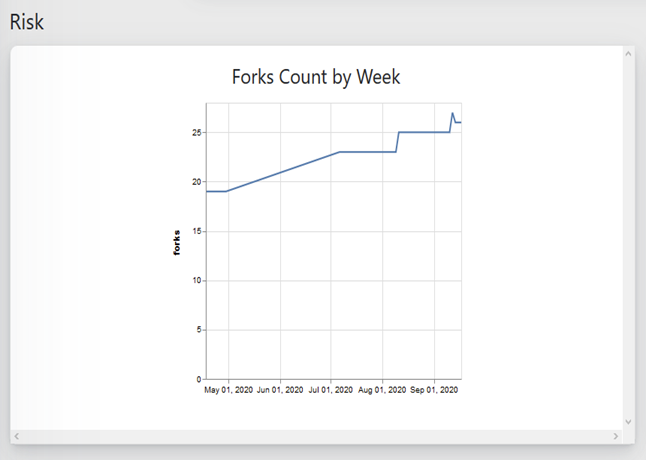
\includegraphics{images/technical-fork_augur-fork.png}

\textbf{GrimoireLab Implementation}\\
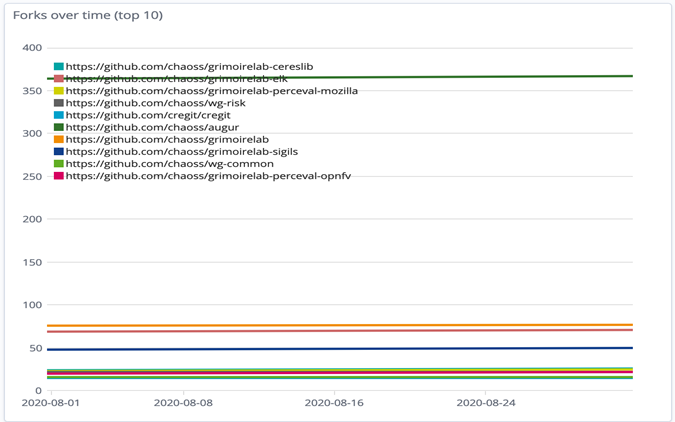
\includegraphics{images/technical-fork_grimoirelab-fork.png}

\hypertarget{tools-providing-the-metric}{%
\subsubsection{Tools Providing the
Metric}\label{tools-providing-the-metric}}

\begin{itemize}
\tightlist
\item
  Augur
\item
  GrimoireLab
\end{itemize}

\hypertarget{data-collection-strategies}{%
\subsubsection{Data Collection
Strategies}\label{data-collection-strategies}}

\textbf{Github API}\\
\url{https://developer.github.com/v3/repos/forks/\#list-forks}

\textbf{GitLab API}\\
\url{https://docs.gitlab.com/ee/api/projects.html\#list-forks-of-a-project}

\textbf{Bitbucket API}\\
\url{https://developer.atlassian.com/bitbucket/api/2/reference/resource/repositories/\%7Bworkspace\%7D/\%7Brepo_slug\%7D/forks}

\hypertarget{references}{%
\subsection{References}\label{references}}

\url{https://help.github.com/en/enterprise/2.13/user/articles/fork-a-repo}
\url{https://opensource.com/article/17/12/fork-clone-difference}
 
\hypertarget{types-of-contributions}{%
\section{Types of Contributions}\label{types-of-contributions}}

Question: What types of contributions are being made?

\hypertarget{description}{%
\subsection{Description}\label{description}}

Multiple, varied contributions make an open source project healthy. Many
projects have community members who do not write code but contribute in
equally valuable ways by managing the community, triaging bugs,
evangelizing the project, supporting users, or helping in other ways.

\hypertarget{objectives}{%
\subsection{Objectives}\label{objectives}}

A variety of contribution types can demonstrate that a project is mature
and well-rounded with sufficient activity to support all aspects of the
project, and enable paths to leadership that are supportive of a variety
of contribution types and people with varying expertise beyond coding.

\hypertarget{implementation}{%
\subsection{Implementation}\label{implementation}}

How contributions are defined, quantified, tracked and made public is a
challenging question. Answers may be unique to each project and the
following suggestions are a starting point. As a general guideline, it
is difficult to compare different contribution types with each other and
they might better be recognized independently.

\begin{itemize}
\tightlist
\item
  The following list can help with identifying contribution types:

  \begin{itemize}
  \tightlist
  \item
    Writing Code
  \item
    Reviewing Code
  \item
    Bug Triaging
  \item
    Quality Assurance and Testing
  \item
    Security-Related Activities
  \item
    Localization/L10N and Translation
  \item
    Event Organization
  \item
    Documentation Authorship
  \item
    Community Building and Management
  \item
    Teaching and Tutorial Building
  \item
    Troubleshooting and Support
  \item
    Creative Work and Design
  \item
    User Interface, User Experience, and Accessibility
  \item
    Social Media Management
  \item
    User Support and Answering Questions
  \item
    Writing Articles
  \item
    Public Relations - Interviews with Technical Press
  \item
    Speaking at Events
  \item
    Marketing and Campaign Advocacy
  \item
    Website Development
  \item
    Legal Council
  \item
    Financial Management
  \end{itemize}
\end{itemize}

\hypertarget{data-collection-strategies}{%
\subsubsection{Data Collection
Strategies}\label{data-collection-strategies}}

\begin{itemize}
\tightlist
\item
  \textbf{Interview or Survey:} Ask community members to recognize
  others for their contributions to recognize contribution types that
  have previously not been considered.

  \begin{itemize}
  \tightlist
  \item
    Who in the project would you like to recognize for their
    contributions? What did they contribute?
  \end{itemize}
\item
  \textbf{Observe project:} Identify and recognize leads of different
  parts of the project.

  \begin{itemize}
  \tightlist
  \item
    What leaders are listed on the project website or in a repository?
  \end{itemize}
\item
  \textbf{Capture Non-code Contributions:} Track contributions through a
  dedicated system, e.g., an issue tracker.

  \begin{itemize}
  \tightlist
  \item
    Logging can include custom information a project wants to know about
    non-code contributions to recognize efforts.
  \item
    Proxy contributions through communication channel activity. For
    example, If quality assurance members (QA) have their own mailing
    list, then activity around QA contributions can be measured by proxy
    from mailing list activity.
  \end{itemize}
\item
  \textbf{Collect Trace Data:} Measure contributions through
  collaboration tool log data.

  \begin{itemize}
  \tightlist
  \item
    For example, code contributions can be counted from a source code
    repository, wiki contributions can be counted from a wiki edit
    history, and email messages can be counted from an email archive
  \end{itemize}
\item
  \textbf{Automate Classification:} Train an artificial intelligence
  (AI) bot to detect and classify contributions.

  \begin{itemize}
  \tightlist
  \item
    An AI bot can assist in categorizing contributions, for example,
    help requests vs. support provided, or feature request vs. bug
    reporting, especially if these are all done in the same issue
    tracker.
  \end{itemize}
\end{itemize}

\emph{Other considerations:}

\begin{itemize}
\tightlist
\item
  Especially with automated reports, allow community members to opt-out
  and not appear on the contribution reports.
\item
  Acknowledge imperfect capture of contribution types and be explicit
  about what types of contributions are included.
\item
  As a project evolves, methods for collecting types of contributions
  will need to adapt. For example, when an internationalization library
  is exchanged, project activity around localization conceivably
  produces different metrics before and after the change.
\item
  Account for activity from bots when mining contribution types at large
  scale.
\end{itemize}

\hypertarget{references}{%
\subsection{References}\label{references}}

\begin{itemize}
\tightlist
\item
  \url{https://medium.com/@sunnydeveloper/revisiting-the-word-recognition-in-foss-and-the-dream-of-open-credentials-d15385d49447}
\item
  \url{https://24pullrequests.com/contributing}
\item
  \url{https://smartbear.com/blog/test-and-monitor/14-ways-to-contribute-to-open-source-without-being/}
\item
  \url{https://wiki.openstack.org/wiki/AUCRecognition}
\item
  \url{https://www.drupal.org/drupalorg/blog/a-guide-to-issue-credits-and-the-drupal.org-marketplace}
\end{itemize}
 
 

\subsection{Focus Area - when}
\textbf{Goal:} 
\begin{table}[ht!]
    \centering
    \begin{tabular}{|p{0.35\linewidth} | p{0.6\linewidth}|}
        \hline
        \hfil \textbf{Metric}  & \hfil \textbf{Question} \\
        \hline
		Activity Dates and Times & What are the dates and timestamps of when contributor activities occur? \\ 
		\hline
		Burstiness & How are short timeframes of intense activity, followed by a corresponding return to a typical pattern of activity, observed in a project? \\ 
		\hline
		Review Cycle Duration within a Change Request & What is the duration of a review cycle within a single change request? \\ 
		\hline
		Time to Close & How much time passes between creating and closing an operation such as an issue, change request, or support ticket? \\ 
		\hline
		Time to First Response & How much time passes between when an activity requiring attention is created and the first response? \\ 
		\hline
    \end{tabular}
\end{table}
 

\subsection{Focus Area - Who}
\textbf{Goal:} Understand organizational and personal engagement with open source projects
\begin{table}[ht!]
    \centering
    \begin{tabular}{|p{0.35\linewidth} | p{0.6\linewidth}|}
        \hline
        \hfil \textbf{Metric}  & \hfil \textbf{Question} \\
        \hline
		Contributor Location & What is the location of contributors? \\ 
		\hline
		Contributors & Who are the contributors to a project? \\ 
		\hline
		Organizational Diversity & What is the organizational diversity of contributions? \\ 
		\hline
    \end{tabular}
\end{table}

\hypertarget{contributor-location}{%
\section{Contributor Location}\label{contributor-location}}

Question: What is the location of contributors?

\hypertarget{description}{%
\subsection{Description}\label{description}}

Geographical location from which contributors contribute, where they
live, or where they work.

\hypertarget{objectives}{%
\subsection{Objectives}\label{objectives}}

To determine global locations of contributors in an effort to understand
work practices and times zones. To identify where contributions do not
come from in an effort to improve engagement in these areas.

\hypertarget{implementation}{%
\subsection{Implementation}\label{implementation}}

\hypertarget{filters}{%
\subsubsection{Filters}\label{filters}}

Filter contributions by:

\begin{itemize}
\tightlist
\item
  \textbf{Location.} Attempt to group locations in regions to have
  multiple levels of reporting. Location is a purposely ambiguous term
  in this context, and could refer to region, country, state, locale, or
  time zone.
\item
  \textbf{Period of time.} Start and finish date of the period. Default:
  forever. Period during which contributions are counted.
\item
  \textbf{Type of contributor}, for example:

  \begin{itemize}
  \tightlist
  \item
    Repository authors
  \item
    Issue authors
  \item
    Code review participants
  \item
    Mailing list authors
  \item
    Event participants
  \item
    IRC authors
  \item
    Blog authors
  \item
    By release cycle
  \item
    Programming languages of the project
  \item
    Role or function in project
  \end{itemize}
\end{itemize}

\hypertarget{visualizations}{%
\subsubsection{Visualizations}\label{visualizations}}

Dot Density Map:

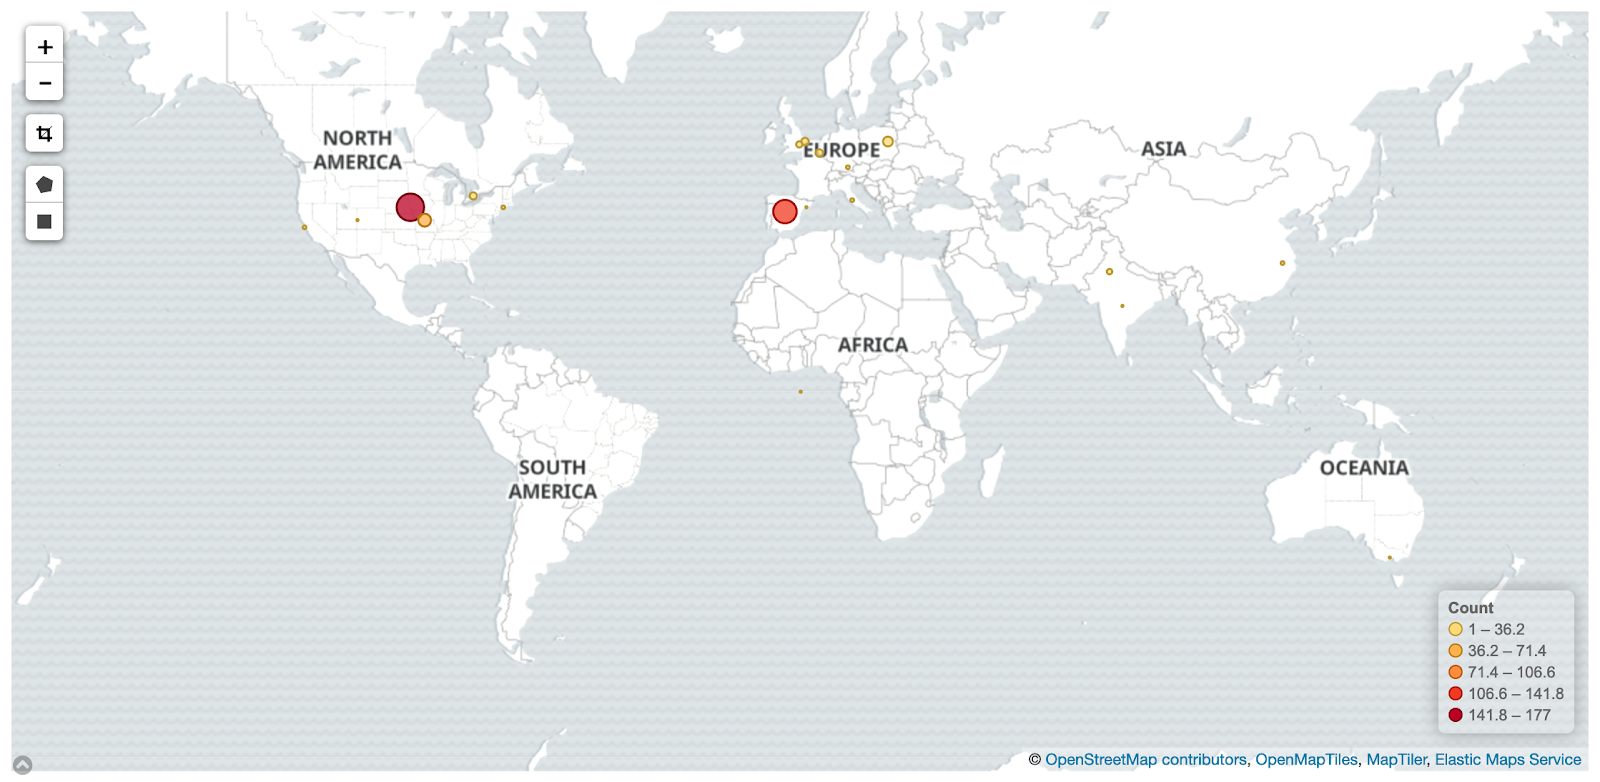
\includegraphics{images/contributor-location_dot-density-map.png}

Source:
\href{https://chaoss.biterg.io/goto/a62f3584a41c1c4c1af5d04b9809a860}{\url{https://chaoss.biterg.io/goto/a62f3584a41c1c4c1af5d04b9809a860}}

Visual heat map:

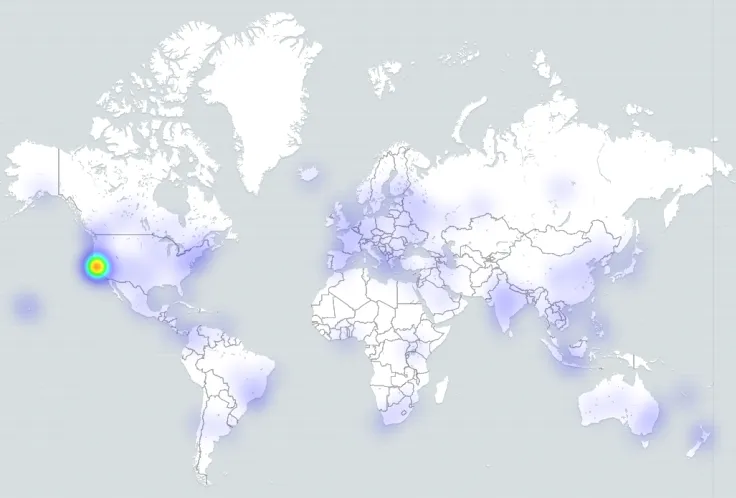
\includegraphics{images/contributor-location_heatmap.png}

Source:
\href{https://blog.bitergia.com/2018/11/20/ubers-community-software-development-analytics-for-open-source-offices}{\url{https://blog.bitergia.com/2018/11/20/ubers-community-software-development-analytics-for-open-source-offices}}

\hypertarget{tools-providing-the-metric}{%
\subsubsection{Tools providing the
metric}\label{tools-providing-the-metric}}

\begin{itemize}
\tightlist
\item
  GrimoireLab
\item
  Augur
\end{itemize}

\hypertarget{data-collection-strategies}{%
\subsubsection{Data Collection
Strategies}\label{data-collection-strategies}}

Different approaches can be used to collect information about location:

\begin{itemize}
\tightlist
\item
  Collect the location information from a contributor's profile in the
  system of engagement.
\item
  Use IP address geolocation of the most frequent locations that
  contributions are made.
\item
  Infer geographical location from the timestamp in contributions.
\item
  Survey contributors.
\end{itemize}

The key challenge for collecting data is determining the location of the
contributor. Best practice would be to leverage any profile information
available from the system of engagement, and if that is not available
then use IP geolocation to determine the most frequent location of
contribution from that individual. Note that contributors may enter in
their profile information false or nonsensical location information
(e.g., ``Earth'' or ``Internet''). Note that IP geolocation can provide
large numbers of false positives due to use of VPNs or other IP masking
tools.

An additional consideration would be the use of external data collection
tools such as community surveys or event registration data that could
cross reference systems of engagement profiles. Contributor location
data could be collected inline with event
\href{https://chaoss.community/metric-attendee-demographics/}{attendee
demographics} and
\href{https://chaoss.community/metric-speaker-demographics/}{speaker
demographics}.

\hypertarget{references}{%
\subsection{References}\label{references}}

\begin{itemize}
\tightlist
\item
  Gonzalez-Barahona, J. M., Robles, G., Andradas-Izquierdo, R., \&
  Ghosh, R. A. (2008). Geographic origin of libre software developers.
  \emph{Information Economics and Policy}, \emph{20}(4), 356-363.
\end{itemize}
 
\hypertarget{contributors}{%
\section{Contributors}\label{contributors}}

Question: Who are the contributors to a project?

\hypertarget{description}{%
\subsection{Description}\label{description}}

A contributor is defined as anyone who contributes to the project in any
way. This metric ensures that all types of contributions are fully
recognized in the project.

\hypertarget{objectives}{%
\subsection{Objectives}\label{objectives}}

Open source projects are comprised of a number of different
contributors. Recognizing all contributors to a project is important in
knowing who is helping with such activities as code development, event
planning, and marketing efforts.

\hypertarget{implementation}{%
\subsection{Implementation}\label{implementation}}

Collect author names from collaboration tools a project uses.

\textbf{Aggregators:}

\begin{itemize}
\tightlist
\item
  Count. Total number of contributors during a given time period.
\end{itemize}

\textbf{Parameters:}

\begin{itemize}
\tightlist
\item
  Period of time. Start and finish date of the period. Default: forever.
  Period during which contributions are counted.
\end{itemize}

\hypertarget{filters}{%
\subsubsection{Filters}\label{filters}}

By location of engagement. For example:

\begin{itemize}
\tightlist
\item
  Commit authors
\item
  Issue authors
\item
  Review participants, e.g., in pull requests
\item
  Mailing list authors
\item
  Event participants
\item
  IRC authors
\item
  Blog authors
\item
  By release cycle
\item
  Timeframe of activity in the project, e.g, find new contributors
\item
  Programming languages of the project
\item
  Role or function in project
\end{itemize}

\hypertarget{visualizations}{%
\subsubsection{Visualizations}\label{visualizations}}

\begin{itemize}
\tightlist
\item
  List of contributor names (often with information about their level of
  engagement)
\end{itemize}

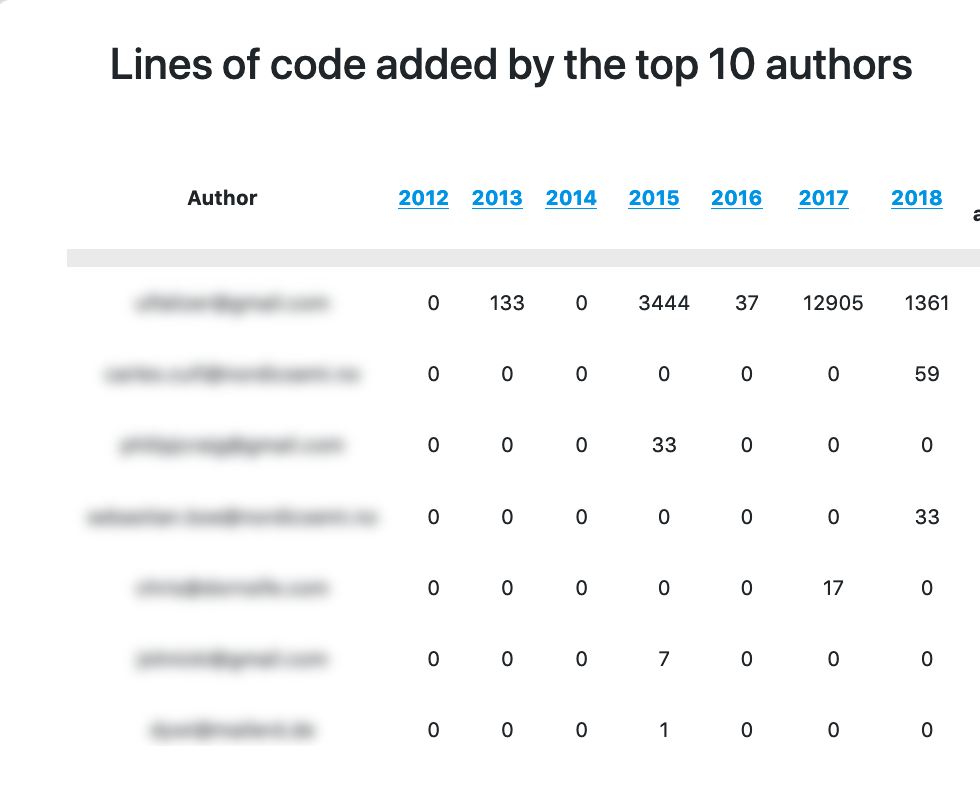
\includegraphics{images/contributors_top-contributor-info.png}

\begin{itemize}
\tightlist
\item
  Summary number of contributors
\end{itemize}

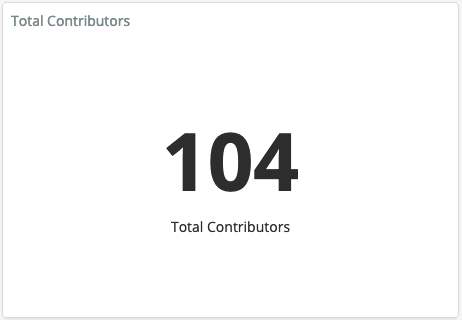
\includegraphics{images/contributors_summary-contributor-number.png}

\begin{itemize}
\tightlist
\item
  Change in the number of active contributors over time
\end{itemize}

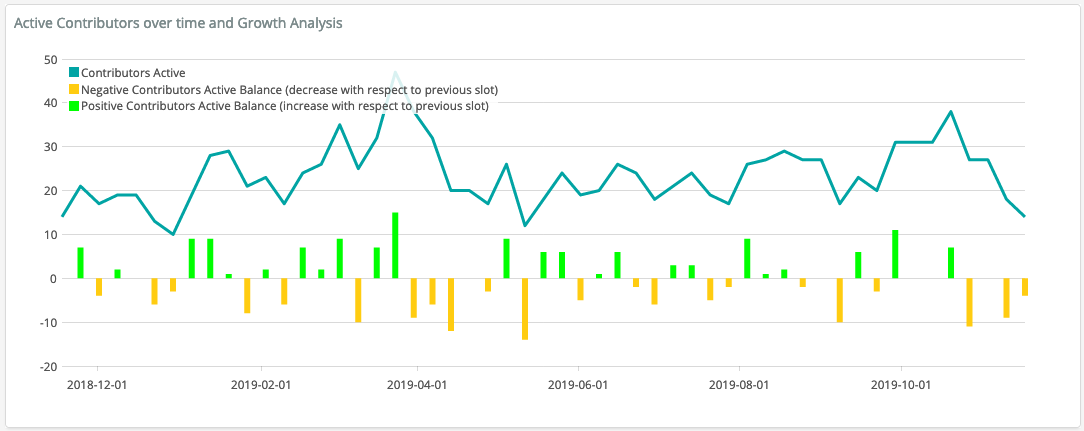
\includegraphics{images/contributors_growth.png}

\begin{itemize}
\tightlist
\item
  New contributors (sort list of contributors by date of first
  contribution)
\end{itemize}

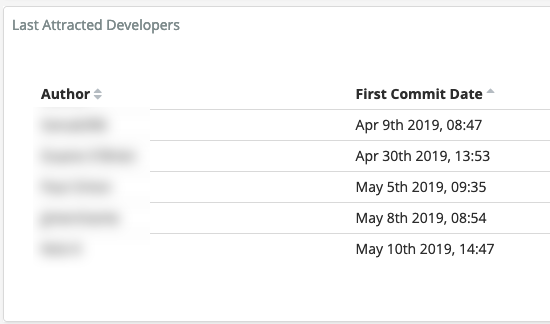
\includegraphics{images/contributors_first-commit-date.png}

\hypertarget{tools-providing-the-metric}{%
\subsubsection{Tools Providing the
Metric}\label{tools-providing-the-metric}}

\begin{itemize}
\tightlist
\item
  \href{https://chaoss.github.io/grimoirelab/}{GrimoireLab}
\item
  \href{http://augur.osshealth.io/api_docs/\#api-Evolution-Contributors_Repo_}{Augur}
\end{itemize}

\hypertarget{data-collection-strategies}{%
\subsubsection{Data Collection
Strategies}\label{data-collection-strategies}}

As indicated above, some contributor information is available via
software such as GrimoireLab and Augur. However, some contributor
insights are less easily obtained via trace data. In these cases,
surveys with community members or event registrations can provide the
desired information. Sample questions include:

\begin{itemize}
\tightlist
\item
  Interview question: Which contributors do not typically appear in
  lists of contributors?
\item
  Interview question: Which contributors are often overlooked as
  important contributors because their contributions are more ``behind
  the scenes''?
\item
  Interview question: What other community members do you regularly work
  with?
\end{itemize}

Additionally, surveys with community members can provide insight to
learn more about contributions to the project. Sample questions include:

\begin{itemize}
\tightlist
\item
  Likert scale {[}1-x{]} item: I am contributing to the project
\item
  Matrix survey item: How often do you engage in the following
  activities in the project?

  \begin{itemize}
  \tightlist
  \item
    Column headings: Never, Rarely(less than once a month), Sometimes
    (more than once a month), Often(once a week or more)
  \item
    Rows include: a) Contributing/reviewing code, b) Creating or
    maintaining documentation, c) Translating documentation, d)
    Participating in decision making about the project's development, e)
    Serving as a community organizer, f) Mentoring other contributors,
    g) Attending events in person, h) Participating through school or
    university computing programs, i) Participating through a program
    like Outreachy, Google Summer of Code, etc., j) Helping with the ASF
    operations (e.g., board meetings or fundraising)
  \end{itemize}
\end{itemize}

\hypertarget{references}{%
\subsection{References}\label{references}}
 
\hypertarget{organizational-diversity}{%
\section{Organizational Diversity}\label{organizational-diversity}}

Question: What is the organizational diversity of contributions?

\hypertarget{description}{%
\subsection{Description}\label{description}}

Organizational diversity expresses how many different organizations are
involved in a project and how involved different organizations are
compared to one another.

\hypertarget{objectives}{%
\subsection{Objectives}\label{objectives}}

\begin{itemize}
\tightlist
\item
  Get a list of organizations contributing to a project.
\item
  See the percentage of contributions from each organization within a
  defined period of time.
\item
  See the change of composition of organizations within a defined period
  of time.
\item
  Get a list of people that are associated with each organization.
\end{itemize}

\hypertarget{implementation}{%
\subsection{Implementation}\label{implementation}}

\begin{itemize}
\tightlist
\item
  Collect data from data sources where contributions occur.
\item
  Identify contributor affiliations to get a good estimate of which
  organizations they belong to.
\item
  Correlate information about contributions, assigning each to
  appropriate organization.
\item
  Depending on the needs of the project, you may want to consider such
  issues as how to handle multiple email addresses, affiliation changes
  over time, or contractor vs. employee.
\end{itemize}

\hypertarget{tools-providing-the-metric}{%
\subsubsection{Tools Providing the
Metric}\label{tools-providing-the-metric}}

\begin{itemize}
\tightlist
\item
  \href{https://chaoss.github.io/grimoirelab}{GrimoireLab} supports
  organizational diversity metrics out of the box. The
  \href{https://github.com/chaoss/grimoirelab-sortinghat}{GrimoireLab
  SortingHat} manages identities. The
  \href{https://github.com/chaoss/grimoirelab-hatstall}{GrimoireLab
  Hatstall} user interface allows correcting organizational affiliation
  of people and even recording affiliation changes.

  \begin{itemize}
  \tightlist
  \item
    View an example visualization on the
    \href{https://chaoss.biterg.io/app/kibana\#/dashboard/Community-Structure-by-Organization}{CHAOSS
    instance of Bitergia Analytics}.
  \item
    Download and import a ready-to-go dashboard containing examples for
    this metric visualization from the
    \href{https://chaoss.github.io/grimoirelab-sigils/panels/community-structure-by-organization/}{GrimoireLab
    Sigils panel collection}.
  \item
    Add a sample visualization to any GrimoreLab Kibiter dashboard
    following these instructions:

    \begin{itemize}
    \tightlist
    \item
      Create a new Pie chart

      \begin{itemize}
      \tightlist
      \item
        Select the \texttt{all\_onion} index
      \item
        Metrics Slice Size: \texttt{Sum} Aggregation,
        \texttt{contributions} Field, \texttt{Contributions} Custom
        Label
      \item
        Buckets Split Slices: \texttt{Terms} Aggregation,
        \texttt{author\_or\_name} Field, \texttt{metric:\ Contributions}
        Order By, \texttt{Descending} Order, \texttt{500} Size,
        \texttt{Organization} Custom Label
      \end{itemize}
    \item
      Example Screenshot
    \end{itemize}

    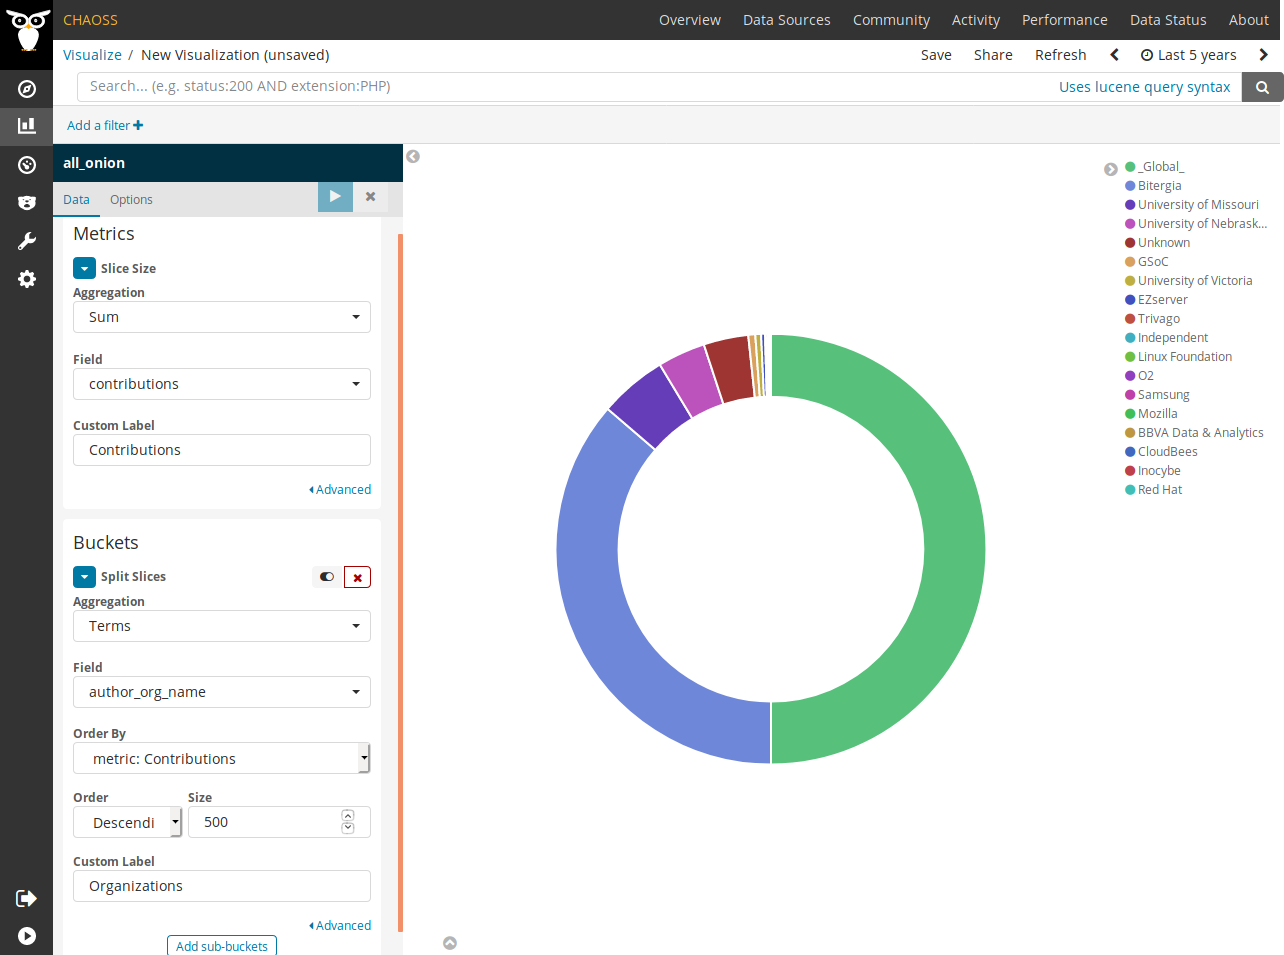
\includegraphics{images/organizational-diversity_piechart.png}
  \end{itemize}
\item
  \href{https://lfanalytics.io}{LF Analytics} provides organization
  diversity metrics in the primary view for commits, issues filed, and
  communication channels (current support for Slack and groups.io)
\end{itemize}

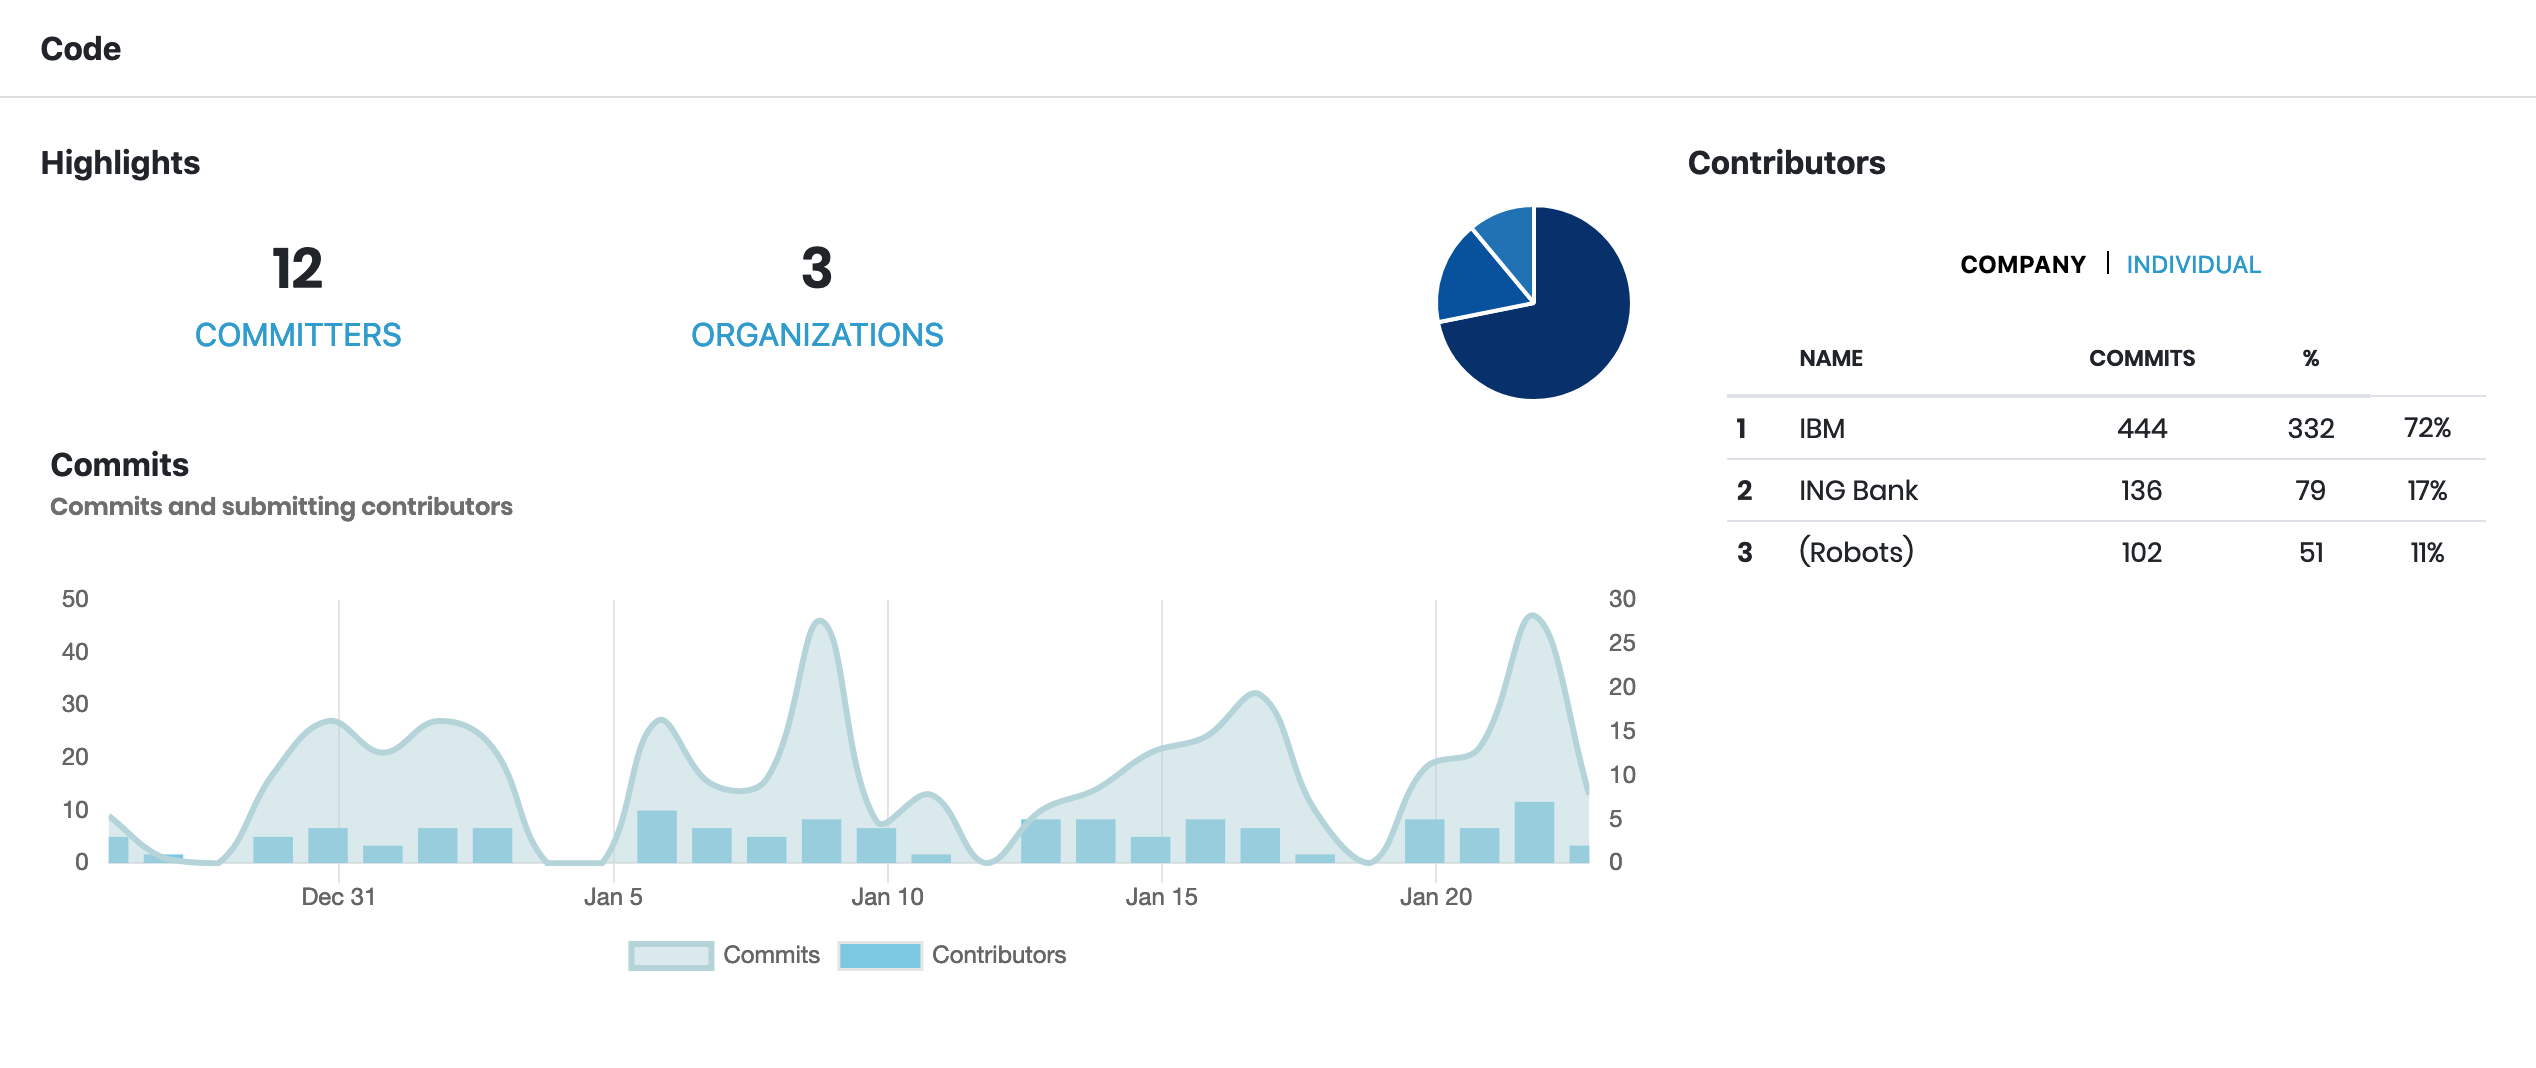
\includegraphics{images/organizational-diversity_lfanalytics-orgdiversity.png}

\hypertarget{data-collection-strategies}{%
\subsubsection{Data Collection
Strategies}\label{data-collection-strategies}}

\textbf{Qualitative}

\begin{itemize}
\tightlist
\item
  Footprint of an organization in a project or ecosystem
\item
  Influence of an organization in a project or ecosystem
\item
  Affiliation diversity in governance structures.
\end{itemize}

\textbf{Quantitative}

\begin{itemize}
\tightlist
\item
  \% of commits by each organization
\item
  \% of merges/reviews from each organization
\item
  \% of any kind of contributors from each organization
\item
  \% of lines of code contributed by each organization
\item
  \% issues filed by each organization
\item
  \href{https://github.com/chaoss/metrics/blob/master/activity-metrics/contributing-organizations.md}{Contributing
  Organizations} - What is the number of contributing organizations?
\item
  \href{https://github.com/chaoss/metrics/blob/master/activity-metrics/new-contributing-organizations.md}{New
  Contributing Organizations} - What is the number of new contributing
  organizations?
\item
  New Contributor Organizations - New organizations contributing to the
  project over time.
\item
  Number of Contributing Organizations - Number of organizations
  participating in the project over time.
\item
  Elephant Factor - If 50\% of community members are employed by the
  same company, it is the elephant in the room. Formally: The minimum
  number of companies whose employees perform 50\% of the commits
\item
  \href{https://github.com/chaoss/metrics/blob/master/activity-metrics/contributor-diversity.md}{Affiliation
  Diversity} - Ratio of contributors from a single company over all
  contributors. Also described as: Maintainers from different companies.
  Diversity of contributor affiliation.
\item
  In projects with the concept of code ownership, \% of code owners
  affiliated with each organization weighed by the importance/size/LoC
  of the code they own and the number of co-owners.
\end{itemize}

\hypertarget{references}{%
\subsection{References}\label{references}}

\begin{itemize}
\tightlist
\item
  Potential implementations and references:

  \begin{itemize}
  \tightlist
  \item
    \url{https://bitergia.gitlab.io/panel-collections/open_source_program_office/organizational-diversity.html}
  \item
    \href{https://katacontainers.biterg.io}{Kata Containers dashboard
    entry page} (bottom of this)
  \item
    \href{https://github.com/chaoss/augur}{Augur}
  \end{itemize}
\end{itemize}
 
 
 


\hypertarget{project-popularity}{%
\section{Project Popularity}\label{project-popularity}}

Question: How popular is an open source project?

\hypertarget{description}{%
\subsection{Description}\label{description}}

Project popularity can be measured by how much activity is visible
around a project. Popularity has a positive feedback loop in which more
popular projects get more attention, attract more users or developers,
and see increases in popularity, spinning the popularity wheel.

Project popularity may be used as a proxy for understanding project
value because open source project economic value is hard to measure, due
to a lack of available usage or sales information for open source
projects.

\hypertarget{objectives}{%
\subsection{Objectives}\label{objectives}}

In a quest to earn a living wage, and to maximize future employment
opportunities, workers may be interested in knowing which projects are
growing and are underserved. Similarly, from an organizational
perspective, knowing which projects are highly used can be helpful in
knowing which projects might be worth investing in. The Project
Popularity metric can be used to identify the trajectory of a project's
development.

\hypertarget{implementation}{%
\subsection{Implementation}\label{implementation}}

The project popularity metric is often considered with changes over
time. There are numerous example vectors to consider when measuring
project popularity based on the number of:

\begin{enumerate}
\def\labelenumi{\arabic{enumi}.}
\tightlist
\item
  Social media mentions
\item
  Forks
\item
  \href{https://chaoss.community/metric-change-requests/}{Change
  requests}
\item
  \href{https://chaoss.community/metric-issues-new/}{New Issues}
\item
  Stars, badges, likes
\item
  \href{https://chaoss.community/metric-new-contributors/}{New
  contributors}
\item
  \href{https://chaoss.community/metric-organizational-diversity/}{Organizational
  Diversity}
\item
  Job postings requesting skills in project
\item
  Conversations within and outside of project
\item
  Clones
\item
  Followers
\item
  Downstream dependencies
\item
  People attending events that focus on a project
\end{enumerate}

\hypertarget{visualizations}{%
\subsubsection{Visualizations}\label{visualizations}}

Issues and reviews (change requests) visualization from Cauldron
(GrimoireLab):

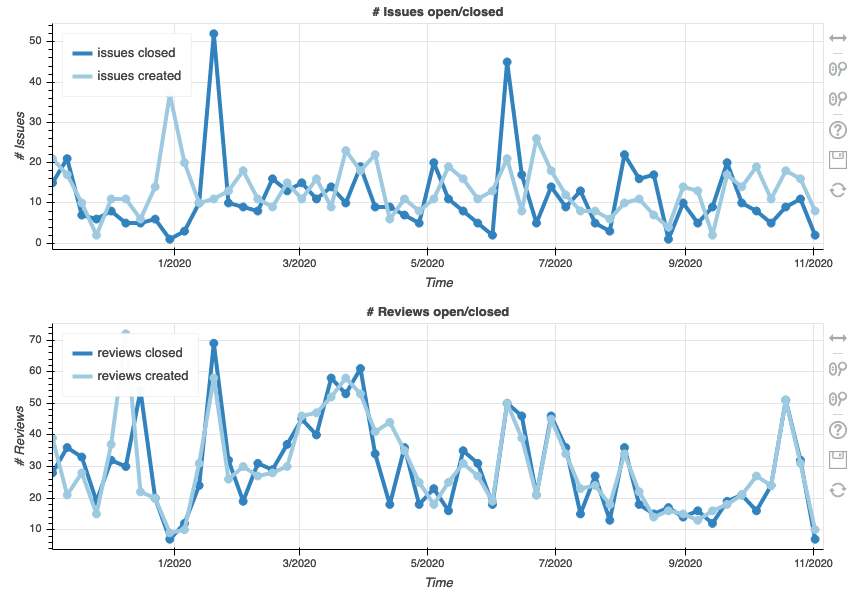
\includegraphics{images/project-popularity_issues-and-reviews.png}

Kubernetes project popularity statistics from DevStats:

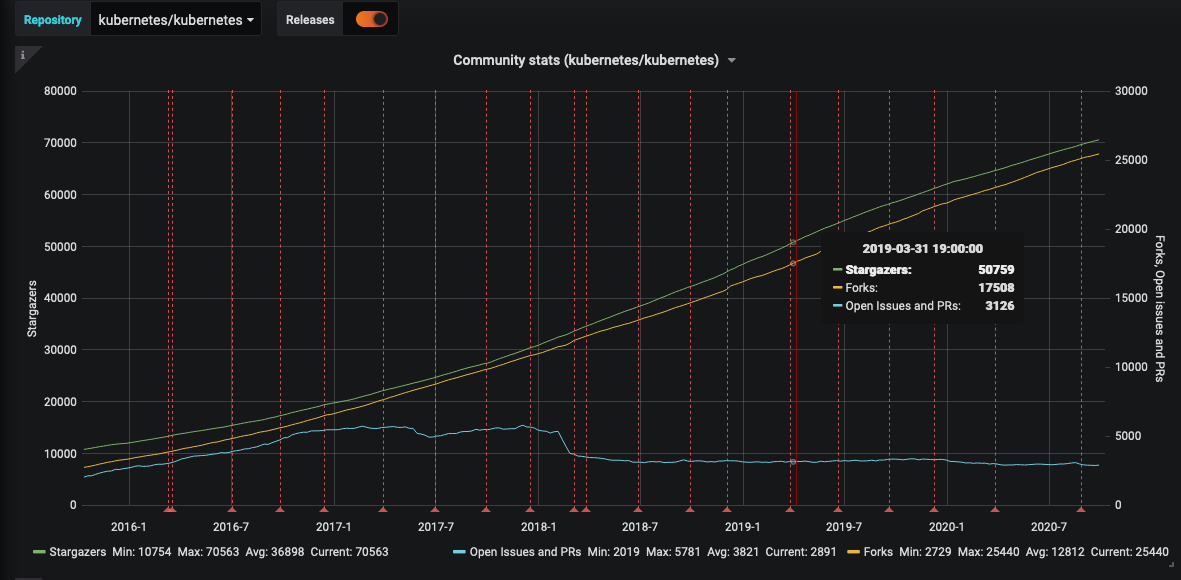
\includegraphics{images/project-popularity_kubernetes.png}

\hypertarget{tools-providing-the-metric}{%
\subsubsection{Tools Providing the
Metric}\label{tools-providing-the-metric}}

\begin{itemize}
\tightlist
\item
  \href{https://github.com/chaoss/augur}{Augur}
\item
  \href{https://chaoss.github.io/grimoirelab/}{GrimoireLab}
\item
  \href{https://cauldron.io/}{Cauldron}
\end{itemize}

\hypertarget{references}{%
\subsection{References}\label{references}}

\begin{itemize}
\tightlist
\item
  \href{http://blog.honeypot.io/most-exciting-open-source-projects-2018/}{Popular
  OpenSource Projects}
\item
  \href{https://isitmaintained.com/}{Is It Maintained?}
\item
  \href{https://github.blog/2018-02-08-open-source-project-trends-for-2018/}{Open
  Source Project Trends}
\item
  \href{https://www.payscale.com/research/US/Skill=Kubernetes/Salary}{Kubernetes
  Salary}
\end{itemize}
 
\hypertarget{project-velocity}{%
\section{Project Velocity}\label{project-velocity}}

Question: What is the development speed for an organization?

\hypertarget{description}{%
\subsection{Description}\label{description}}

Project velocity is the number of issues, the number of pull requests,
volume of commits, and number of contributors as an indicator of
'innovation'.

\hypertarget{objectives}{%
\subsection{Objectives}\label{objectives}}

Gives an Open Source Program Office (OSPO) manager a way to compare the
project velocity across a portfolio of projects.

The OSPO manager can use the Project Velocity metric to:

\begin{itemize}
\tightlist
\item
  Report project velocity of open source projects vs in-house projects
\item
  Compare project velocity across a portfolio of projects
\item
  Identify which projects grow beyond internal contributors (when
  filtering internal vs. external contributors)
\item
  Identify promising areas in which to get involved
\item
  Highlight areas likely to be the successful platforms over the next
  several years
\end{itemize}

\href{https://www.cncf.io/blog/2017/06/05/30-highest-velocity-open-source-projects}{See
Example}

\hypertarget{implementation}{%
\subsection{Implementation}\label{implementation}}

Base metrics include:

\begin{itemize}
\tightlist
\item
  \href{https://github.com/chaoss/wg-evolution/blob/master/metrics/Issues_Closed.md}{issues
  closed}
\item
  \href{https://github.com/chaoss/wg-evolution/blob/master/metrics/Reviews.md}{number
  of reviews}
\item
  \href{https://github.com/chaoss/wg-evolution/blob/master/metrics/Code_Changes.md}{\#
  of code changes}
\item
  \href{https://github.com/chaoss/wg-risk/blob/master/metrics/Committers.md}{\#
  of committers}
\end{itemize}

\hypertarget{filters}{%
\subsubsection{Filters}\label{filters}}

\begin{itemize}
\tightlist
\item
  Internal vs external contributors
\item
  Project sources (e.g., internal repositories, open-source
  repositories, and competitor open-source repositories)
\item
  Time
\end{itemize}

\hypertarget{visualizations}{%
\subsubsection{Visualizations}\label{visualizations}}

\begin{itemize}
\tightlist
\item
  X-Axis: Logarithmic scale for Code Changes
\item
  Y-Axis: Logarithmic scale of Sum of Number of Issues and Number of
  Reviews
\item
  Dot-size: Committers
\item
  Dots are projects
\end{itemize}

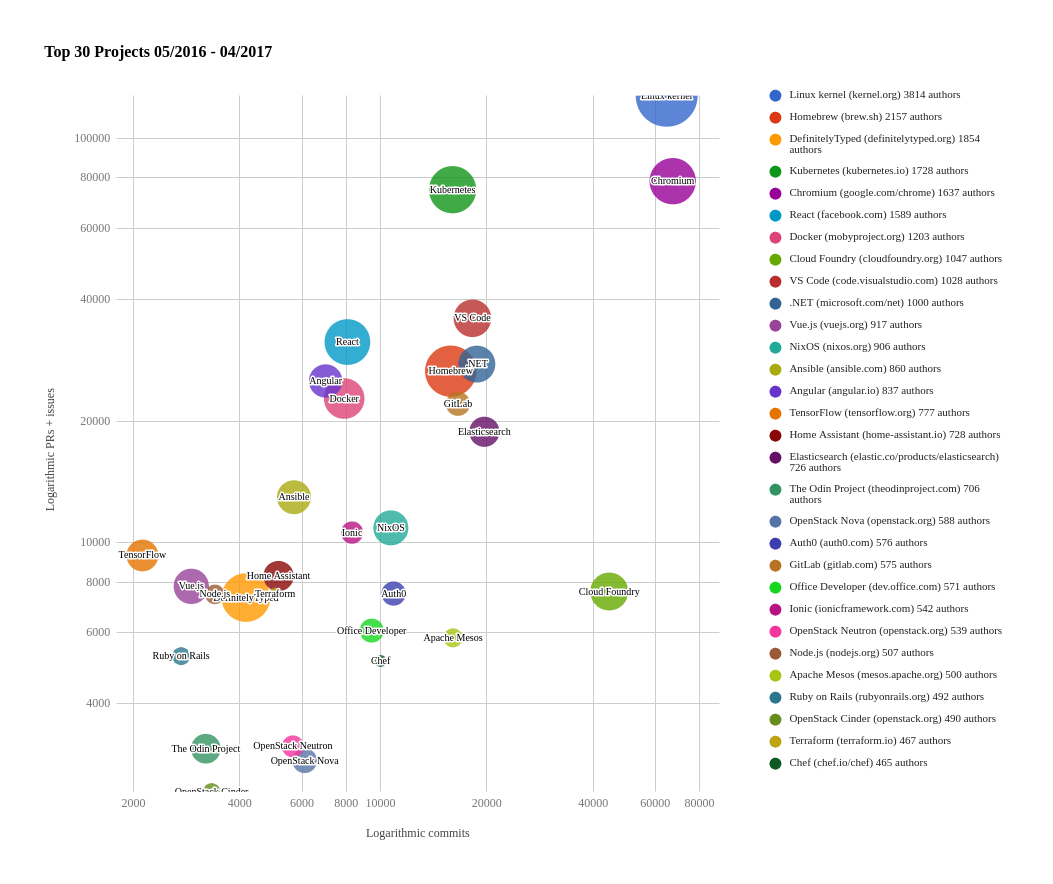
\includegraphics{images/project-velocity_visualization.png}

\href{https://www.cncf.io/blog/2017/06/05/30-highest-velocity-open-source-projects/}{From
CNCF}

\hypertarget{tools-providing-the-metric}{%
\subsubsection{Tools providing the
Metric}\label{tools-providing-the-metric}}

\begin{itemize}
\tightlist
\item
  CNCF - \url{https://github.com/cncf/velocity}
\end{itemize}

\hypertarget{references}{%
\subsection{References}\label{references}}

\begin{itemize}
\tightlist
\item
  \href{https://www.threefivetwo.com/blog/can-open-source-innovation-work-in-the-enterprise}{Can
  Open Source Innovation work in the Enterprise?}
\item
  \href{https://www.nearform.com/blog/want-a-high-performing-culture-make-way-for-open-innovation}{Open
  Innovation for a High Performance Culture}
\item
  \href{https://www.cio.com/article/3213146/open-source-is-powering-the-digital-enterprise.html}{Open
  Source for the Digital Enterprise}
\item
  \href{https://www.cncf.io/blog/2017/06/05/30-highest-velocity-open-source-projects}{Highest
  Velocity Open Source Projects}
\end{itemize}
 
\hypertarget{social-listening}{%
\subsubsection{Social Listening}\label{social-listening}}

Question: How does one measure the value of community interactions and
accurately gauge ``reputation'' of a community as evident from
qualitative sentiment?

\emph{Note: This metric synthesizes several other metrics that can be
derived from trace data, and several process-oriented metrics. Embedded
footnotes annotate areas planned for later clarification, and questions
for later resolution.}

\hypertarget{description}{%
\paragraph{Description}\label{description}}

Social Listening is a combination of
\href{https://blog.hubspot.com/service/social-listening}{social
listening} practices across multiple channels along with a meaningful
set of categorizations. The combination of these tactics can lead to
systematic community analysis and can inform a community strategy that
leads to measurable business value. 1

\textbf{Theory and Origin}

Social currency or social capital is a social scientific theory. It
broadly considers how human interactions build relationships and trust
in a community. The Social Listening metric represents the reputation of
a community as measured via community trust, transparency, utility,
consistency, and merit.

Interpersonal relationships are the social fabric of communities. This
is shown in the
\href{https://theadminzone.com/ams/levingers-stage-theory.1272/}{Levinger's
Relationship Model} and
\href{https://psycnet.apa.org/record/1973-28661-000}{Social Penetration
Theory}. Community members' sense of personal and group identity grows
as they interact. Members build shared values, accumulate a sense of
trust, encourage cooperation, and garner reciprocity through acts of
\href{https://en.wikipedia.org/wiki/Self-disclosure}{self-disclosure}.
These interactions build an increased and measurable sense of
connection. The measure of these characteristics is called social
currency. 2

\textbf{Results}

The Social Listening metric is a way to sort through a fire hose of
qualitative data from community interactions. A central premise of this
approach is that community members' interactions have an impact on the
community. The Social Listening metric continually measures the
sentiment 3 from those interactions. It illustrates the reputation and
level of trust between community members and leaders. 4

\hypertarget{objectives}{%
\paragraph{Objectives}\label{objectives}}

Analyze the qualitative comments in community interactions. Gain an
overview of sentiment in a community. Get metrics that show at a glance
how a community is and was doing. Use lead metrics from continuous
measurements for proactive community strategy development. Instill trust
in community members that their thoughts and opinions are valued.

\hypertarget{implementation}{%
\paragraph{Implementation}\label{implementation}}

The Social Listening requires the collection of community comments
(communication traces), the definition of a codex, and the on-going
review of the communication traces. 5

Set up a Data Collection Platform of your choice as described in the
``Tools'' section below. Ensure it has a minimum of 4 dimensions and 3
communication channels. Once it is set up, the following method is used
to collect, analyze, and interpret results:


\includegraphics{images/social-listening_circle2.png}

\begin{enumerate}
\def\labelenumi{\arabic{enumi}.}
\item
  \textbf{Collect Communication Traces} -\/- Identify online platforms
  that your community is communicating on. Set up data funnels from the
  primary platform to your Social Listening tool. The critical data for
  the system is user generated content.
\item
  \textbf{Standardize How Communication Traces Should Be Assessed} -\/-
  Use a codex to define important concepts as a ``tracking keyword'' or
  ``category'' in the focal community. This unified codex of terms
  ensures consistent analysis as different people read and tag community
  sentiment. Formalizing the revision and addition structure to this
  codex on a regular basis is a must. 5
\item
  \textbf{Analyze the Communication Traces} -\/- Community sentiment is
  analyzed in the Social Listening tool by tagging data with codex
  terms. If the tagging is done by a team of people, it is recommended
  that everyone gets together regularly to discuss trends and ensure
  consistent tag use. If the tagging is done by an artificial
  intelligence algorithm, then a human team should supervise and retrain
  the AI as necessary. 5
\item
  \textbf{Share and Visualize the Aggregated Analysis} -\/- Visualize
  the quantitative count of codex terms over time, e.g., in a dashboard.
  This is where the qualitative analysis results produce an easy to
  observe dashboard of trends. Share analysis with team members. 6
\item
  \textbf{Benchmark, Set Goals \& Predict Future Growth} -\/- After
  getting enough data to form a benchmark, take stock of where your
  community stands. What are its strengths and weaknesses? What actions
  can be taken to make the community healthier and more robust? Then
  form community initiatives with well-defined goals and execute on
  these projects to affect the social currency metrics for next week. 6
\item
  \textbf{Repeat the Process} -\/- In regular evaluation meetings,
  discuss the shortcomings of the dataset or collection methods. Come up
  with methods to address these shortcomings in the future. Work
  solutions into the system and move forward. Truth is in the trend,
  power is in the pattern.7
\end{enumerate}

\hypertarget{filters}{%
\subparagraph{Filters}\label{filters}}

\begin{enumerate}
\def\labelenumi{\arabic{enumi}.}
\tightlist
\item
  \textbf{Channel}: Sort by where the data was collected from.
\item
  \textbf{Tag}: Show data based on what codex tags were used to identify
  sentiment in comments.
\item
  \textbf{Time}: Show trends in the data over time and pull specific
  data-sets.
\item
  \textbf{Most impactful comments}: Sort and filter by flags that can be
  placed in the data to highlight specific data points and explain their
  importance.
\item
  \textbf{AI vs. Human tagged}: Filter by whether tags were applied
  programmatically or by a person.
\item
  \textbf{Weighted currency:} Weight the ``importance'' of certain
  comments based on any one individually selected criteria. A resulting
  weighted view is simply a re-order of information based on weight.
\end{enumerate}

\hypertarget{visualizations}{%
\subparagraph{Visualizations}\label{visualizations}}

\textbf{Dashboard visualizing the aggregate metrics:}

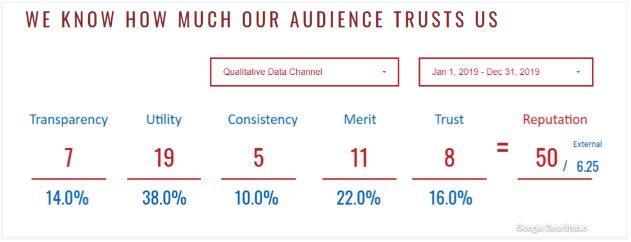
\includegraphics{images/social-listening_dashboard.png}

\textbf{Example Social Listening tool:} On the left, raw community
comments are shown and tags are added in columns immediately to the
right. On the right, a pivot table shows in numbers how often tags
occurred in combination with other tags.

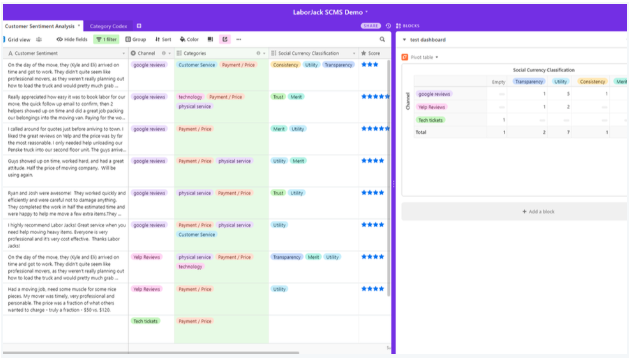
\includegraphics{images/social-listening_tool-example.png}

\textbf{Expanded comments view:} remove the ``quantitative'' from the
fields and provide the best possible way to read the different comments.

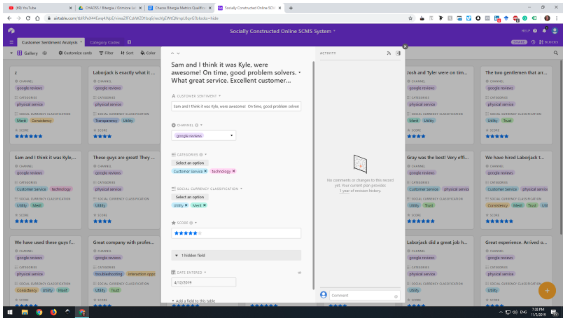
\includegraphics{images/social-listening_expanded-comment.png}

\hypertarget{tools-providing-the-metric}{%
\subparagraph{Tools Providing the
Metric}\label{tools-providing-the-metric}}

To implement the metric any MySQL, smart-sheet, excel, or airtable-like
excel datasheet program works fine. This data should be simplified
enough to interact with other data interfaces to ensure that data
migration is simple, straightforward, and can be automated (such as
google data studio). This requires that systems used to implement the
Social Listening metric work with CSV and other spreadsheet files, and
we heavily recommend open source programs for its implementation.

Once you have this, create a data set with the following data points: 8

\begin{longtable}[]{@{}ll@{}}
\toprule
Data Points & Description \\
\midrule
\endhead
Date of entry & Date data was imported to Social Listening tool \\
Date of comment & Date comment was made on original platform \\
Comment Text & Qualitative data brought in. Decide on how large you want
these chunks ported. Some may port an entire email while others will be
broken into one row per sentence. It should only have one
``sentiment'' \\
Data channel & Originating data channel the comment came from \\
Tags (created on codex document below) & Based on the unified codex of
terms, decide what tags to track. There can be two kinds of tags. On the
one hand, tags can be based on ``themes'' or recurring sentiment that
people voice (e.g., gamer gate, flamewar, or thank you notes). On the
other hand, tags based on ``categories'' can describe different aspects
of a community that members comment on (e.g., events, release, or
governance). \\
Social Currency Metric & The social currency being awarded or demerited
in the system. This will directly affect numbers. \\
Weighted Score & Once you've decided what your ``weight'' will be, you
can assign a system of -3 to +3 to provide a weighted view of
human-tagged metrics (AI will not assign a weight for several reasons).
This enables the ``most impactful comment'' filter. \\
\bottomrule
\end{longtable}

Create a second sheet for the Unified Codex of Terms which will define
terms. It should look like this: 8

\begin{longtable}[]{@{}llll@{}}
\toprule
Category Term & Definition & When to use & When not~to use \\
\midrule
\endhead
{[}Custom Tags - themes and categories{]} & & & \\
{[}Community specific jargon{]} & & & \\
Social Currency Dimensions: & & & \\
TRANSPARENCY & Do people recognize and feel a connection to your
community?~ & When they have the "words" to pinpoint why they feel you
are authentic or personable. & This is not about good customer service,
or doing well. That is utility. This is about whether they understand
who you are as a business and show they are onboard with it. \\
UTILITY & Is your community doing something useful or is it contributing
value? & Provide parameters that exclude when the term is used so that
people know when the category tag should not be implemented. & This is
not about good customer service, or doing well. That is utility. This is
about whether they understand who you are as a business and show they
are onboard with it. \\
CONSISTENCY & Do you have a history of being reliable and dependable? &
When they suggest they have used your brand, or interacted with you
several times & If they've only provided their comment to suggest you
were useful once, use utility instead. \\
MERIT & Does your community merit respect and attention for your
accomplishments? & When the social currency garnered from customers
seems it will continue for a while, and will impact other people's
opinions. & When they suggest they will use you again in the future use
trust instead as that is a personal trust in the brand. Merit is
external. \\
TRUST & Can people trust that your community will continue to provide
value and grow in the future? & When they suggest they trust you well
enough to continue conversations with you in the future & When there is
not substantial enough evidence to suggest they will continue to work
with and trust you as a loyal customer or community member. \\
INTERNAL REPUTATION 9 & Do people believe these things strongly enough
to warrant conversation or action? & & \\
EXTERNAL REPUTATION 9 & What amount of your reputation in your community
is transferable to strangers outside of your community (cold audiences)?
& & \\
\bottomrule
\end{longtable}

The codex is filled in by stakeholders on a regular basis by specific
communities and forms the basis for analysis of the data. This is the
MOST IMPORTANT part. Without this the subjectivity of qualitative data
does not follow the rule of generalization: 9

\begin{quote}
``A concept applies to B population ONLY SO FAR AS C limitation.''
\end{quote}

\hypertarget{data-collection-strategies}{%
\subparagraph{Data Collection
Strategies}\label{data-collection-strategies}}

Community member comments are available from trace data. The Social
Listening metric ideally imports the comment text automatically into a
tool for tagging. Trace data can be collected from a communities'
collaboration platforms where members write comments, including
ticketing systems, code reviews, email lists, instant messaging, social
media, and fora.

\textbf{Legal and Regulatory Considerations}

\emph{Points of destruction}: Detailed data is destroyed after \emph{xx}
months has passed. Quantitative calculations are kept for up to 250
weeks per GDPR compliance. Data older than 250 weeks becomes archived
data you cannot manipulate but can see. Users can negotiate the primary
statistic.

\hypertarget{references}{%
\paragraph{References}\label{references}}

\begin{itemize}
\tightlist
\item
  \href{https://airtable.com/invite/l?inviteId=inv8u49VVMtQTrfFU\&inviteToken=c49b1ed3759c5cd736901fd81c9f460f86e8e9f462703c4f85a3bdd7250ca5a7}{An
  example implementation on airtable}
\item
  \href{https://datastudio.google.com/open/1X9UdQz8FtHHmjMBpjba3pFqE55lNpwg5}{An
  example implementation in data studio}(report)
\item
  \href{https://datastudio.google.com/open/1Z4EJ03898lZxm2NZVULaEoLS0bYqL79A}{An
  example implementation in data studio} (data source)
\item
  \href{https://drive.google.com/open?id=1zi3JE0bwfEdRdc-wQEZn8GaB7sE8IvxeSeqvVywKnXw}{An
  example implementation in google sheets}
\item
  \href{https://docs.google.com/document/d/1RlAedRBQbhq0oYMCB3VqdawOCZE2XT5R3teydjBZODM/edit\#heading=h.8hyunaadfriq}{Implementation
  documentation} (starts on page 33)
\end{itemize}

\hypertarget{annotated-footnotes}{%
\paragraph{Annotated Footnotes}\label{annotated-footnotes}}

1 CHAOSS metrics historically is to create standard definitions that can
be used reliably across projects to support comparisons. This metric may
evolve into a project in the future.

2 What metrics emerge from this description? Likely included are: 1.
community trust, 2. transparency, 3. utility, 4. consistency, and 5.
merit

3 Analysis of sentiment suggests that metric (6) is likely
"Communications Sentiment", and the definition may need to include
references to common sentiment analysis tools, sometimes called "bags of
words".

4 Measuring how trust trust is instilled in community members, such that
their thoughts and opinions are valued is likely metric (7) that will
define a process, and perhaps is not measurable via trace data.

5 A substantial portion of any codex for open source software will be
common across projects, and each project is likely to have a set of
particular interests that are a subset of that codex. In some cases,
their main interests may not be present in an established codex
component. In general, the codex, like the CHAOSS project itself, is
open sourced as shared metadata to ensure shared understanding across
open source communities.

6 This describes the evolution of a standard codex, and its elements
through the process of CHAOSS working groups and projects, characterized
in the previous footnote. Likely this will be a process metric (8).

7 Candidate process oriented metric (9).

8 Examples of data coded using the open sourced codex, as it evolves,
will be essential components for advancing open source software through
Social Listening. Implementations will require these examples, and their
provision as open source assets of the CHAOSS project will return value
as shared data.

9 Internal and external reputation are likely metrics (10), and (11)
arising from the Social Listening metric.
 
 

\hypertarget{job-opportunities}{%
\section{Job Opportunities}\label{job-opportunities}}

Question: How many job postings request skills with technologies from a
project?

\hypertarget{description}{%
\subsection{Description}\label{description}}

A common way for open source contributors to earn a living wage is to be
employed by a company or be a self-employed or freelance developer.
Skills in a specific project may improve a job applicant's prospects of
getting a job. The most obvious indicator for demand related to a skill
learned in a specific open source project is when that project or its
technology is included in job postings.

\hypertarget{objectives}{%
\subsection{Objectives}\label{objectives}}

The metric gives contributors a sense of how much skills learned in a
specific open source project are valued by companies.

\hypertarget{implementation}{%
\subsection{Implementation}\label{implementation}}

To obtain this metric on a job search platform (e.g., LinkedIn, Indeed,
or Dice), go to the job search and type in the name of the open source
project. The number of returned job postings is the metric. Periodically
collecting the metric through an API of a job search platform and
storing the results allows to see trends.

\hypertarget{filters}{%
\subsubsection{Filters}\label{filters}}

\begin{itemize}
\tightlist
\item
  Age of job posting; postings get stale and may not be removed when
  filled
\end{itemize}

\hypertarget{visualizations}{%
\subsubsection{Visualizations}\label{visualizations}}

The metric can be extended by looking at:

\begin{itemize}
\tightlist
\item
  Salary ranges for jobs returned
\item
  Level of seniority for jobs returned
\item
  Availability of jobs like on-site or off-site
\item
  Location of job
\item
  Geography
\end{itemize}

\hypertarget{references}{%
\subsection{References}\label{references}}

\begin{itemize}
\tightlist
\item
  LinkedIn Job Search API:
  \url{https://developer.linkedin.com/docs/v1/jobs/job-search-api\#}
\item
  Indeed Job Search API:
  \url{https://opensource.indeedeng.io/api-documentation/docs/job-search/}
\item
  Dice.com Job Search API:
  \url{http://www.dice.com/external/content/documentation/api.html}
\item
  Monster Job Search API: \url{https://partner.monster.com/job-search}
\item
  Ziprecruiter API (Requires Partnership):
  \url{https://www.ziprecruiter.com/zipsearch}
\end{itemize}

\emph{Note:} This metric is limited to individual projects but
engagement in open source can be beneficial for other reasons. This
metric could be tweaked to look beyond a single project and instead use
related skills such as programming languages, processes, open source
experience, or frameworks as search parameters for jobs.
 
\hypertarget{organizational-project-skill-demand}{%
\subsubsection{Organizational Project Skill
Demand}\label{organizational-project-skill-demand}}

Question: How many organizations are using this project and could hire
me if I become proficient?

\hypertarget{description}{%
\paragraph{Description}\label{description}}

Organizations engage with open source projects through use and
dependencies. This metric is aimed at determining downstream demand of
skills related to an open source project. This metric looks at
organizations that deploy a project as part of an IT infrastructure,
other open source projects with declared dependencies, and references to
the project through social media, conference mentions, blog posts, and
similar activities.

\hypertarget{objectives}{%
\paragraph{Objectives}\label{objectives}}

As a developer, I'd like to invest my skills and time in a project that
has a likelihood of getting me a decent paying job in the future. People
can use the Downstream Organizational Impact of a Project Software
metric to discover which projects are used by organizations, and they
may, therefore, be able to pursue job opportunities with, possibly
requiring IT support services.

\hypertarget{implementation}{%
\paragraph{Implementation}\label{implementation}}

Base metrics include:

\begin{itemize}
\tightlist
\item
  Number of organizations that created issues for a project
\item
  Number of organizations that created pull requests for a project
\item
  Number of organizations that blog or tweet about a project
\item
  Number of organizations that mention a project in open hiring requests
\item
  Number of organizations that are represented at meetups about this
  project
\item
  Number of other projects that are dependent on a project
\item
  Number of books about a project
\item
  Google search trends for a project
\end{itemize}

\hypertarget{visualizations}{%
\subparagraph{Visualizations}\label{visualizations}}

The following visualization demonstrates the number of downstream
projects dependendent on the project in question. While this
visualization does not capture the entirety of the Downstream
Organizational Impact of a Project Software metric, it provides a visual
for a portion.

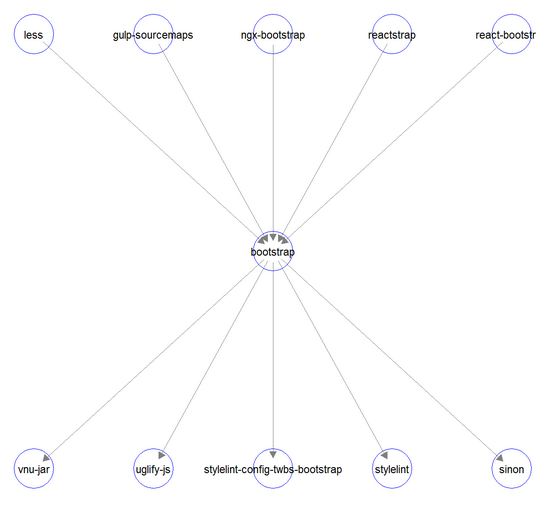
\includegraphics{images/organizational-project-skill-demand_paper.png}

Other visualizations could include Google search trends (React vs.
Angular vs. Vue.js)

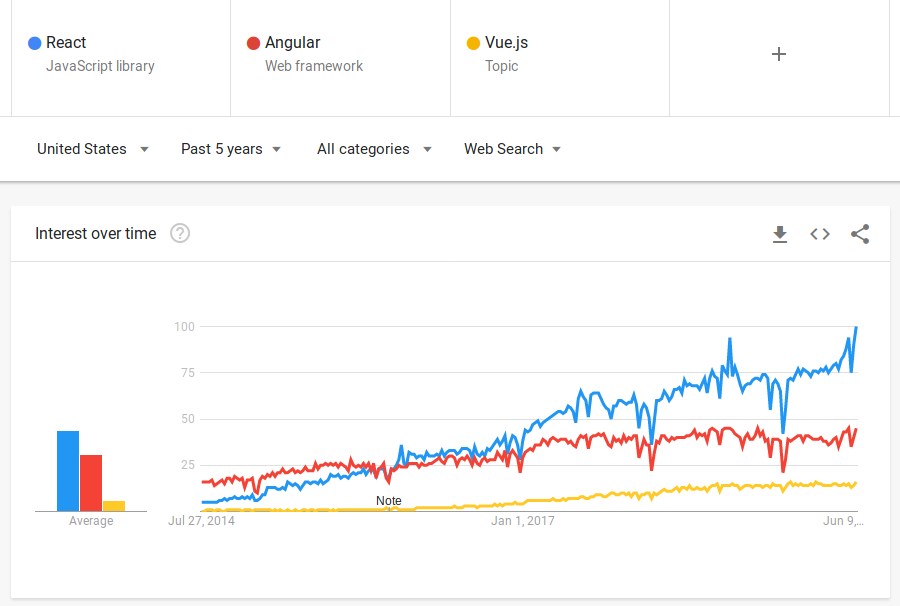
\includegraphics{images/organizational-project-skill-demand_google-trends.png}

ThoughtWorks publishes a series called 'Tech Radar' that shows the
popularity of technologies.

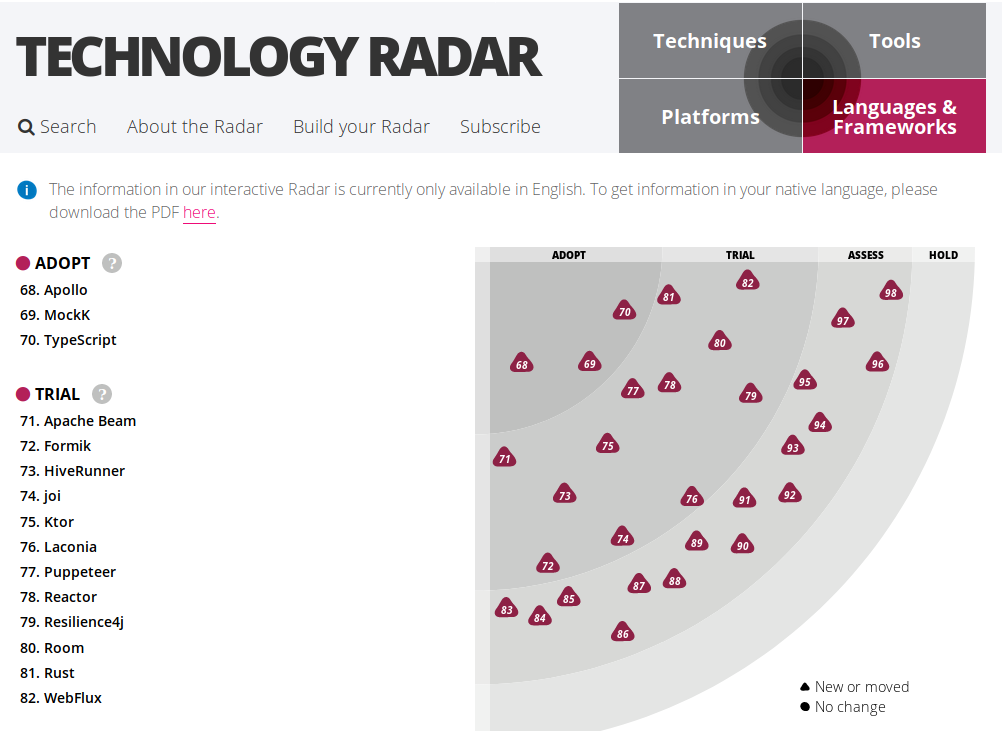
\includegraphics{images/organizational-project-skill-demand_tech-radar.png}

Tech Radar allows you to drill down on projects to see how the
assessment has changed over time.

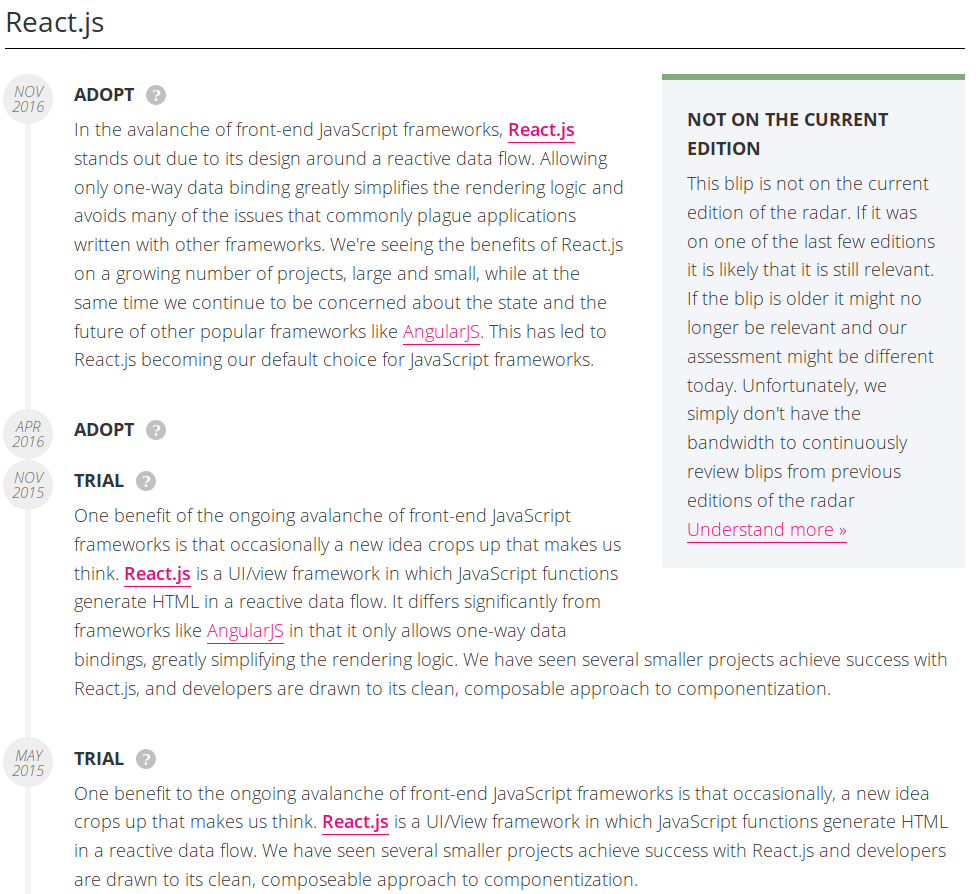
\includegraphics{images/organizational-project-skill-demand_tech-react.png}

StackOverview publishes an annual developer's survey

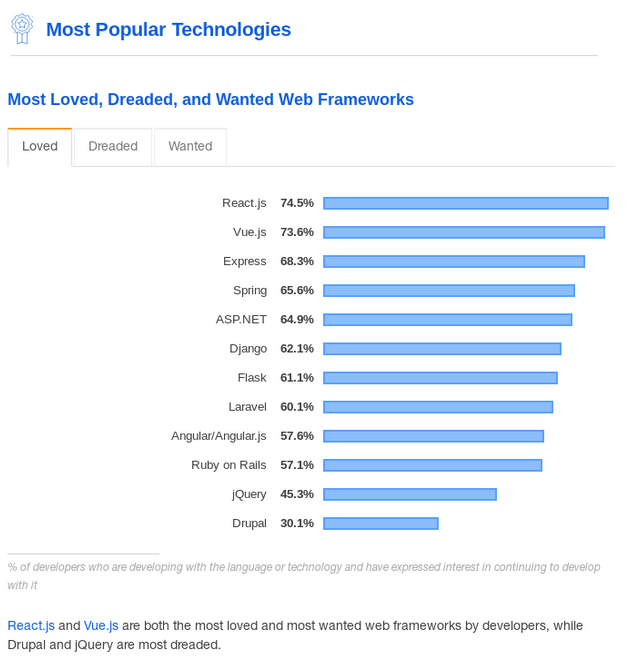
\includegraphics{images/organizational-project-skill-demand_stack-overflow.png}

\hypertarget{tools-providing-the-metric}{%
\subparagraph{Tools Providing the
Metric}\label{tools-providing-the-metric}}

\begin{itemize}
\tightlist
\item
  Google Trends - for showing search interest over time
\item
  ThoughtWorks TechRadar - project assessments from a tech consultancy
\item
  StackOverflow Developer's Survey - annual project rankings
\item
  Augur; Examples are available for multiple repositories:

  \begin{itemize}
  \tightlist
  \item
    \href{http://augur.osshealth.io/repo/Rails\%20(wg-value)/rails/overview}{Rails}
  \item
    \href{http://augur.osshealth.io/repo/Zephyr-RTOS/zephyr/overview}{Zephyr}
  \item
    \href{http://augur.osshealth.io/repo/Apache\%20(wg-value)/cloudstack/overview}{CloudStack}
  \end{itemize}
\end{itemize}

\hypertarget{references}{%
\paragraph{References}\label{references}}

\begin{itemize}
\tightlist
\item
  \href{https://opensource.org/sponsors}{Open Source Sponsors}
\item
  \href{https://opensource.com/article/19/1/fiscal-sponsors-open-source}{Fiscal
  Sponsors and Open Source}
\item
  \href{https://www.networkworld.com/article/2867020/big-names-like-google-dominate-open-source-funding.html}{Large
  Corporate OpenSource Sponsors}
\item
  \href{https://www.npmjs.com/package/google-trends-api}{Google Trends
  API}
\item
  \href{https://aisel.aisnet.org/cgi/viewcontent.cgi?article=1496\&context=amcis2018}{Measuring
  Open Source Software Impact}
\item
  \href{https://www.thoughtworks.com/radar}{ThoughtWorks Tech Radar}
\item
  \href{https://insights.stackoverflow.com/survey/2019\#technology}{Stack
  Overflow Developer's Survey}
\end{itemize}
 
 
 

\end{document}


\subsection{Focus Area - What}
\textbf{Goal:} 
\begin{table}[ht!]
    \centering
    \begin{tabular}{|p{0.35\linewidth} | p{0.6\linewidth}|}
        \hline
        \hfil \textbf{Metric}  & \hfil \textbf{Question} \\
        \hline
		Technical Fork & What are a number of technical forks of an open source project on code development platforms? \\ 
		\hline
		Types of Contributions & What types of contributions are being made? \\ 
		\hline
    \end{tabular}
\end{table}

\hypertarget{technical-fork}{%
\section{Technical Fork}\label{technical-fork}}

Question: What are a number of technical forks of an open source project
on code development platforms?

\hypertarget{description}{%
\subsection{Description}\label{description}}

A technical fork is a distributed version control copy of a project. The
number of technical forks indicates the number of copies of a project on
the same code development platform.

\hypertarget{objectives}{%
\subsection{Objectives}\label{objectives}}

The objective of the Technical Fork metric is to ascertain how many
copies of a project exist on a code development platform. Analysis of
technical forks may provide insight into forking intentions (different
types of forks such as contributing, and non-contributing forks).

\hypertarget{implementation}{%
\subsection{Implementation}\label{implementation}}

\hypertarget{filters}{%
\subsubsection{Filters}\label{filters}}

\begin{itemize}
\tightlist
\item
  Time Period (e.g., Weekly, Monthly, Annually)
\item
  Ratio of contributing fork to total forks (A contributing fork is a
  fork that has opened a change request against the original
  repository.)
\item
  Ratio of non-contributing fork to total forks (A non-contributing fork
  is a fork that has never opened a change request against the original
  repository.)
\end{itemize}

\hypertarget{visualizations}{%
\subsubsection{Visualizations}\label{visualizations}}

\textbf{Augur Implementation}\\
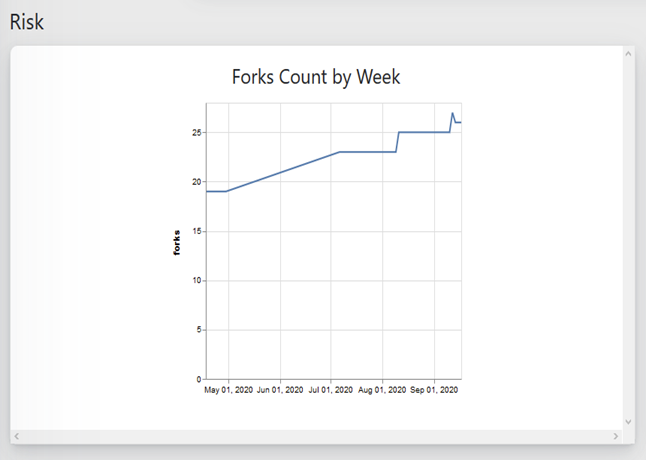
\includegraphics{images/technical-fork_augur-fork.png}

\textbf{GrimoireLab Implementation}\\
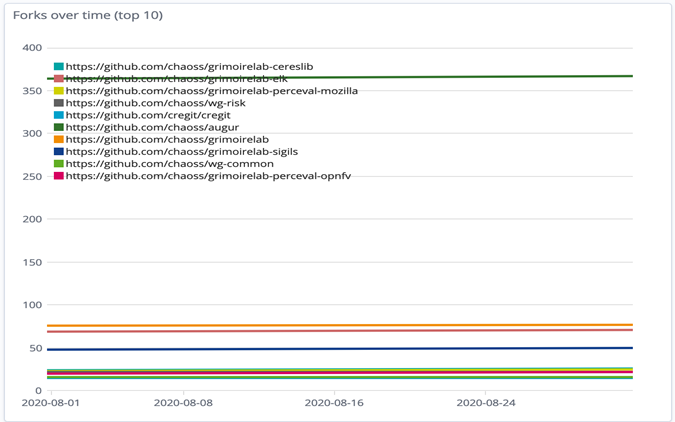
\includegraphics{images/technical-fork_grimoirelab-fork.png}

\hypertarget{tools-providing-the-metric}{%
\subsubsection{Tools Providing the
Metric}\label{tools-providing-the-metric}}

\begin{itemize}
\tightlist
\item
  Augur
\item
  GrimoireLab
\end{itemize}

\hypertarget{data-collection-strategies}{%
\subsubsection{Data Collection
Strategies}\label{data-collection-strategies}}

\textbf{Github API}\\
\url{https://developer.github.com/v3/repos/forks/\#list-forks}

\textbf{GitLab API}\\
\url{https://docs.gitlab.com/ee/api/projects.html\#list-forks-of-a-project}

\textbf{Bitbucket API}\\
\url{https://developer.atlassian.com/bitbucket/api/2/reference/resource/repositories/\%7Bworkspace\%7D/\%7Brepo_slug\%7D/forks}

\hypertarget{references}{%
\subsection{References}\label{references}}

\url{https://help.github.com/en/enterprise/2.13/user/articles/fork-a-repo}
\url{https://opensource.com/article/17/12/fork-clone-difference}
 
\hypertarget{types-of-contributions}{%
\section{Types of Contributions}\label{types-of-contributions}}

Question: What types of contributions are being made?

\hypertarget{description}{%
\subsection{Description}\label{description}}

Multiple, varied contributions make an open source project healthy. Many
projects have community members who do not write code but contribute in
equally valuable ways by managing the community, triaging bugs,
evangelizing the project, supporting users, or helping in other ways.

\hypertarget{objectives}{%
\subsection{Objectives}\label{objectives}}

A variety of contribution types can demonstrate that a project is mature
and well-rounded with sufficient activity to support all aspects of the
project, and enable paths to leadership that are supportive of a variety
of contribution types and people with varying expertise beyond coding.

\hypertarget{implementation}{%
\subsection{Implementation}\label{implementation}}

How contributions are defined, quantified, tracked and made public is a
challenging question. Answers may be unique to each project and the
following suggestions are a starting point. As a general guideline, it
is difficult to compare different contribution types with each other and
they might better be recognized independently.

\begin{itemize}
\tightlist
\item
  The following list can help with identifying contribution types:

  \begin{itemize}
  \tightlist
  \item
    Writing Code
  \item
    Reviewing Code
  \item
    Bug Triaging
  \item
    Quality Assurance and Testing
  \item
    Security-Related Activities
  \item
    Localization/L10N and Translation
  \item
    Event Organization
  \item
    Documentation Authorship
  \item
    Community Building and Management
  \item
    Teaching and Tutorial Building
  \item
    Troubleshooting and Support
  \item
    Creative Work and Design
  \item
    User Interface, User Experience, and Accessibility
  \item
    Social Media Management
  \item
    User Support and Answering Questions
  \item
    Writing Articles
  \item
    Public Relations - Interviews with Technical Press
  \item
    Speaking at Events
  \item
    Marketing and Campaign Advocacy
  \item
    Website Development
  \item
    Legal Council
  \item
    Financial Management
  \end{itemize}
\end{itemize}

\hypertarget{data-collection-strategies}{%
\subsubsection{Data Collection
Strategies}\label{data-collection-strategies}}

\begin{itemize}
\tightlist
\item
  \textbf{Interview or Survey:} Ask community members to recognize
  others for their contributions to recognize contribution types that
  have previously not been considered.

  \begin{itemize}
  \tightlist
  \item
    Who in the project would you like to recognize for their
    contributions? What did they contribute?
  \end{itemize}
\item
  \textbf{Observe project:} Identify and recognize leads of different
  parts of the project.

  \begin{itemize}
  \tightlist
  \item
    What leaders are listed on the project website or in a repository?
  \end{itemize}
\item
  \textbf{Capture Non-code Contributions:} Track contributions through a
  dedicated system, e.g., an issue tracker.

  \begin{itemize}
  \tightlist
  \item
    Logging can include custom information a project wants to know about
    non-code contributions to recognize efforts.
  \item
    Proxy contributions through communication channel activity. For
    example, If quality assurance members (QA) have their own mailing
    list, then activity around QA contributions can be measured by proxy
    from mailing list activity.
  \end{itemize}
\item
  \textbf{Collect Trace Data:} Measure contributions through
  collaboration tool log data.

  \begin{itemize}
  \tightlist
  \item
    For example, code contributions can be counted from a source code
    repository, wiki contributions can be counted from a wiki edit
    history, and email messages can be counted from an email archive
  \end{itemize}
\item
  \textbf{Automate Classification:} Train an artificial intelligence
  (AI) bot to detect and classify contributions.

  \begin{itemize}
  \tightlist
  \item
    An AI bot can assist in categorizing contributions, for example,
    help requests vs. support provided, or feature request vs. bug
    reporting, especially if these are all done in the same issue
    tracker.
  \end{itemize}
\end{itemize}

\emph{Other considerations:}

\begin{itemize}
\tightlist
\item
  Especially with automated reports, allow community members to opt-out
  and not appear on the contribution reports.
\item
  Acknowledge imperfect capture of contribution types and be explicit
  about what types of contributions are included.
\item
  As a project evolves, methods for collecting types of contributions
  will need to adapt. For example, when an internationalization library
  is exchanged, project activity around localization conceivably
  produces different metrics before and after the change.
\item
  Account for activity from bots when mining contribution types at large
  scale.
\end{itemize}

\hypertarget{references}{%
\subsection{References}\label{references}}

\begin{itemize}
\tightlist
\item
  \url{https://medium.com/@sunnydeveloper/revisiting-the-word-recognition-in-foss-and-the-dream-of-open-credentials-d15385d49447}
\item
  \url{https://24pullrequests.com/contributing}
\item
  \url{https://smartbear.com/blog/test-and-monitor/14-ways-to-contribute-to-open-source-without-being/}
\item
  \url{https://wiki.openstack.org/wiki/AUCRecognition}
\item
  \url{https://www.drupal.org/drupalorg/blog/a-guide-to-issue-credits-and-the-drupal.org-marketplace}
\end{itemize}
 
 

\subsection{Focus Area - when}
\textbf{Goal:} 
\begin{table}[ht!]
    \centering
    \begin{tabular}{|p{0.35\linewidth} | p{0.6\linewidth}|}
        \hline
        \hfil \textbf{Metric}  & \hfil \textbf{Question} \\
        \hline
		Activity Dates and Times & What are the dates and timestamps of when contributor activities occur? \\ 
		\hline
		Burstiness & How are short timeframes of intense activity, followed by a corresponding return to a typical pattern of activity, observed in a project? \\ 
		\hline
		Review Cycle Duration within a Change Request & What is the duration of a review cycle within a single change request? \\ 
		\hline
		Time to Close & How much time passes between creating and closing an operation such as an issue, change request, or support ticket? \\ 
		\hline
		Time to First Response & How much time passes between when an activity requiring attention is created and the first response? \\ 
		\hline
    \end{tabular}
\end{table}
 

\subsection{Focus Area - Who}
\textbf{Goal:} Understand organizational and personal engagement with open source projects
\begin{table}[ht!]
    \centering
    \begin{tabular}{|p{0.35\linewidth} | p{0.6\linewidth}|}
        \hline
        \hfil \textbf{Metric}  & \hfil \textbf{Question} \\
        \hline
		Contributor Location & What is the location of contributors? \\ 
		\hline
		Contributors & Who are the contributors to a project? \\ 
		\hline
		Organizational Diversity & What is the organizational diversity of contributions? \\ 
		\hline
    \end{tabular}
\end{table}

\hypertarget{contributor-location}{%
\section{Contributor Location}\label{contributor-location}}

Question: What is the location of contributors?

\hypertarget{description}{%
\subsection{Description}\label{description}}

Geographical location from which contributors contribute, where they
live, or where they work.

\hypertarget{objectives}{%
\subsection{Objectives}\label{objectives}}

To determine global locations of contributors in an effort to understand
work practices and times zones. To identify where contributions do not
come from in an effort to improve engagement in these areas.

\hypertarget{implementation}{%
\subsection{Implementation}\label{implementation}}

\hypertarget{filters}{%
\subsubsection{Filters}\label{filters}}

Filter contributions by:

\begin{itemize}
\tightlist
\item
  \textbf{Location.} Attempt to group locations in regions to have
  multiple levels of reporting. Location is a purposely ambiguous term
  in this context, and could refer to region, country, state, locale, or
  time zone.
\item
  \textbf{Period of time.} Start and finish date of the period. Default:
  forever. Period during which contributions are counted.
\item
  \textbf{Type of contributor}, for example:

  \begin{itemize}
  \tightlist
  \item
    Repository authors
  \item
    Issue authors
  \item
    Code review participants
  \item
    Mailing list authors
  \item
    Event participants
  \item
    IRC authors
  \item
    Blog authors
  \item
    By release cycle
  \item
    Programming languages of the project
  \item
    Role or function in project
  \end{itemize}
\end{itemize}

\hypertarget{visualizations}{%
\subsubsection{Visualizations}\label{visualizations}}

Dot Density Map:

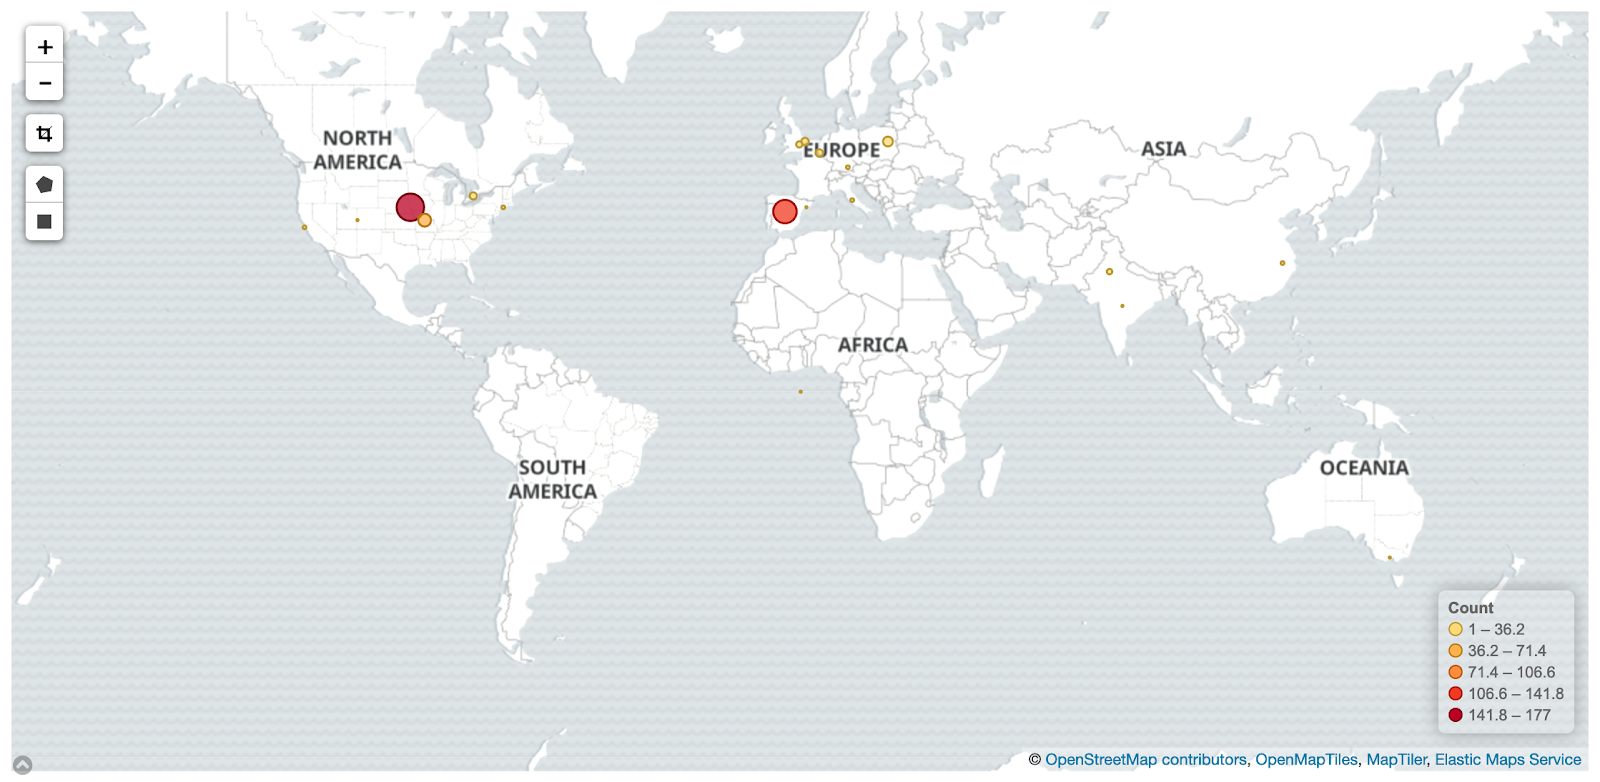
\includegraphics{images/contributor-location_dot-density-map.png}

Source:
\href{https://chaoss.biterg.io/goto/a62f3584a41c1c4c1af5d04b9809a860}{\url{https://chaoss.biterg.io/goto/a62f3584a41c1c4c1af5d04b9809a860}}

Visual heat map:

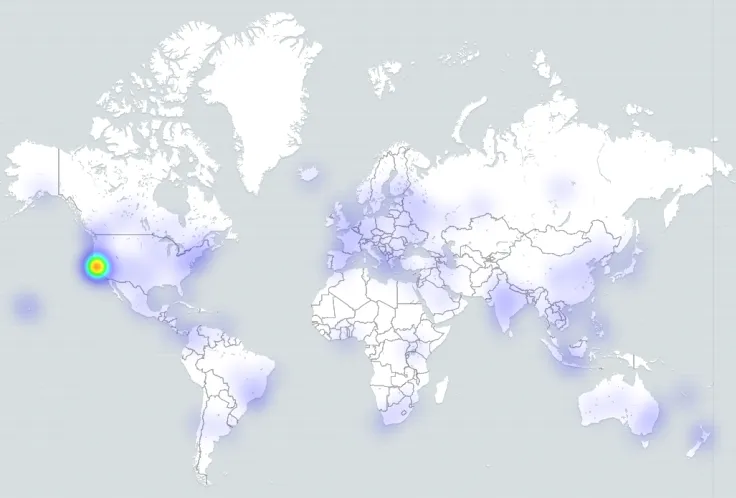
\includegraphics{images/contributor-location_heatmap.png}

Source:
\href{https://blog.bitergia.com/2018/11/20/ubers-community-software-development-analytics-for-open-source-offices}{\url{https://blog.bitergia.com/2018/11/20/ubers-community-software-development-analytics-for-open-source-offices}}

\hypertarget{tools-providing-the-metric}{%
\subsubsection{Tools providing the
metric}\label{tools-providing-the-metric}}

\begin{itemize}
\tightlist
\item
  GrimoireLab
\item
  Augur
\end{itemize}

\hypertarget{data-collection-strategies}{%
\subsubsection{Data Collection
Strategies}\label{data-collection-strategies}}

Different approaches can be used to collect information about location:

\begin{itemize}
\tightlist
\item
  Collect the location information from a contributor's profile in the
  system of engagement.
\item
  Use IP address geolocation of the most frequent locations that
  contributions are made.
\item
  Infer geographical location from the timestamp in contributions.
\item
  Survey contributors.
\end{itemize}

The key challenge for collecting data is determining the location of the
contributor. Best practice would be to leverage any profile information
available from the system of engagement, and if that is not available
then use IP geolocation to determine the most frequent location of
contribution from that individual. Note that contributors may enter in
their profile information false or nonsensical location information
(e.g., ``Earth'' or ``Internet''). Note that IP geolocation can provide
large numbers of false positives due to use of VPNs or other IP masking
tools.

An additional consideration would be the use of external data collection
tools such as community surveys or event registration data that could
cross reference systems of engagement profiles. Contributor location
data could be collected inline with event
\href{https://chaoss.community/metric-attendee-demographics/}{attendee
demographics} and
\href{https://chaoss.community/metric-speaker-demographics/}{speaker
demographics}.

\hypertarget{references}{%
\subsection{References}\label{references}}

\begin{itemize}
\tightlist
\item
  Gonzalez-Barahona, J. M., Robles, G., Andradas-Izquierdo, R., \&
  Ghosh, R. A. (2008). Geographic origin of libre software developers.
  \emph{Information Economics and Policy}, \emph{20}(4), 356-363.
\end{itemize}
 
\hypertarget{contributors}{%
\section{Contributors}\label{contributors}}

Question: Who are the contributors to a project?

\hypertarget{description}{%
\subsection{Description}\label{description}}

A contributor is defined as anyone who contributes to the project in any
way. This metric ensures that all types of contributions are fully
recognized in the project.

\hypertarget{objectives}{%
\subsection{Objectives}\label{objectives}}

Open source projects are comprised of a number of different
contributors. Recognizing all contributors to a project is important in
knowing who is helping with such activities as code development, event
planning, and marketing efforts.

\hypertarget{implementation}{%
\subsection{Implementation}\label{implementation}}

Collect author names from collaboration tools a project uses.

\textbf{Aggregators:}

\begin{itemize}
\tightlist
\item
  Count. Total number of contributors during a given time period.
\end{itemize}

\textbf{Parameters:}

\begin{itemize}
\tightlist
\item
  Period of time. Start and finish date of the period. Default: forever.
  Period during which contributions are counted.
\end{itemize}

\hypertarget{filters}{%
\subsubsection{Filters}\label{filters}}

By location of engagement. For example:

\begin{itemize}
\tightlist
\item
  Commit authors
\item
  Issue authors
\item
  Review participants, e.g., in pull requests
\item
  Mailing list authors
\item
  Event participants
\item
  IRC authors
\item
  Blog authors
\item
  By release cycle
\item
  Timeframe of activity in the project, e.g, find new contributors
\item
  Programming languages of the project
\item
  Role or function in project
\end{itemize}

\hypertarget{visualizations}{%
\subsubsection{Visualizations}\label{visualizations}}

\begin{itemize}
\tightlist
\item
  List of contributor names (often with information about their level of
  engagement)
\end{itemize}

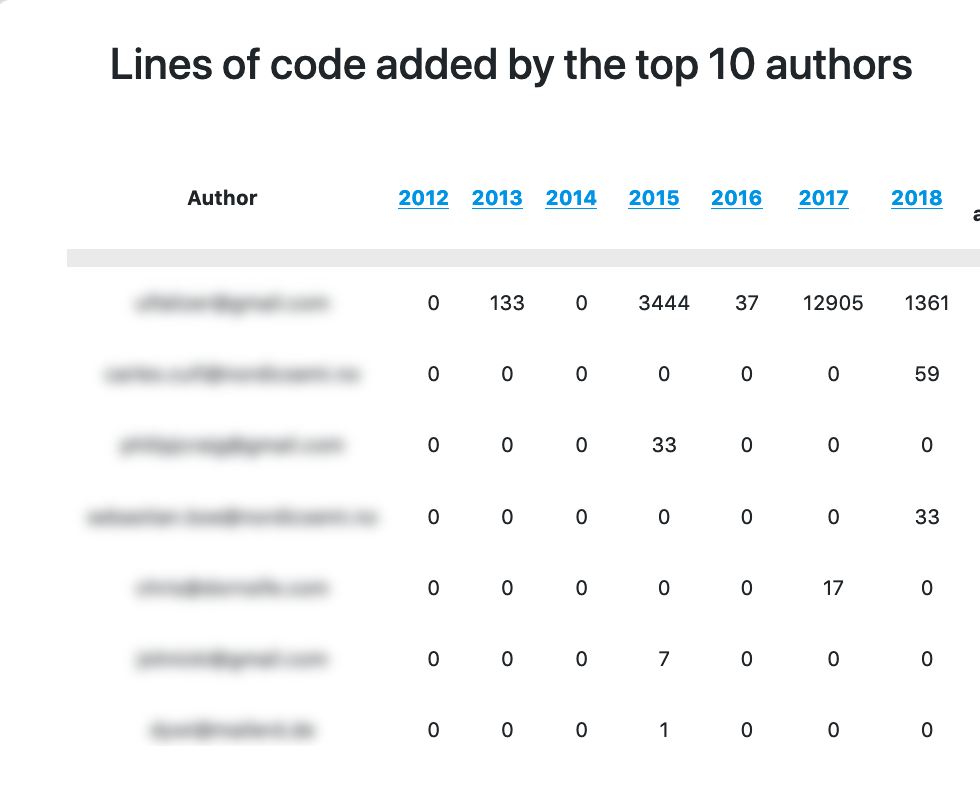
\includegraphics{images/contributors_top-contributor-info.png}

\begin{itemize}
\tightlist
\item
  Summary number of contributors
\end{itemize}

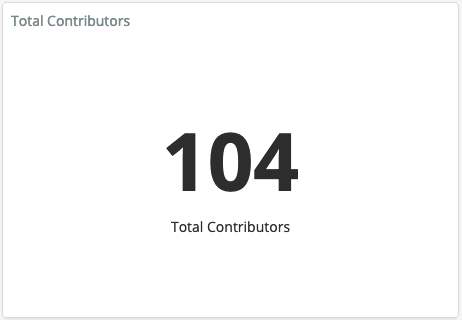
\includegraphics{images/contributors_summary-contributor-number.png}

\begin{itemize}
\tightlist
\item
  Change in the number of active contributors over time
\end{itemize}

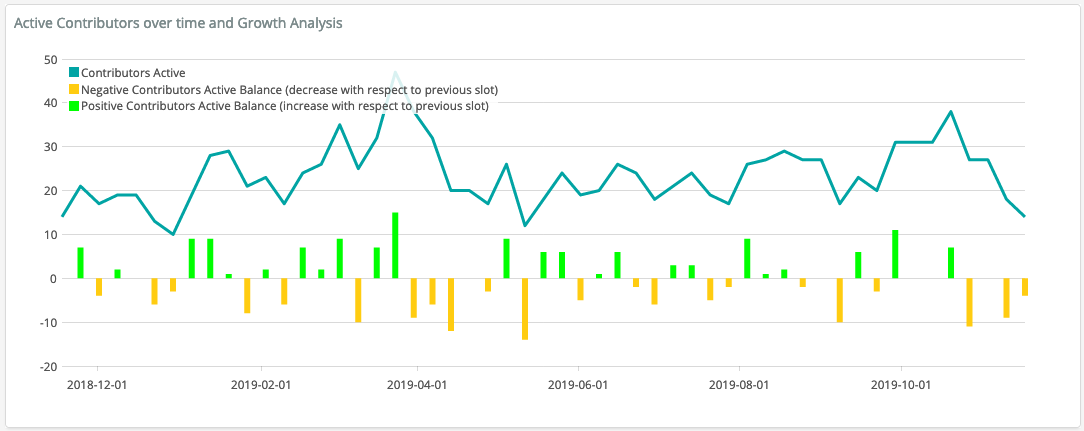
\includegraphics{images/contributors_growth.png}

\begin{itemize}
\tightlist
\item
  New contributors (sort list of contributors by date of first
  contribution)
\end{itemize}

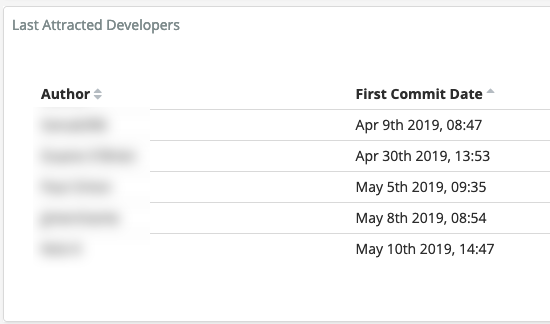
\includegraphics{images/contributors_first-commit-date.png}

\hypertarget{tools-providing-the-metric}{%
\subsubsection{Tools Providing the
Metric}\label{tools-providing-the-metric}}

\begin{itemize}
\tightlist
\item
  \href{https://chaoss.github.io/grimoirelab/}{GrimoireLab}
\item
  \href{http://augur.osshealth.io/api_docs/\#api-Evolution-Contributors_Repo_}{Augur}
\end{itemize}

\hypertarget{data-collection-strategies}{%
\subsubsection{Data Collection
Strategies}\label{data-collection-strategies}}

As indicated above, some contributor information is available via
software such as GrimoireLab and Augur. However, some contributor
insights are less easily obtained via trace data. In these cases,
surveys with community members or event registrations can provide the
desired information. Sample questions include:

\begin{itemize}
\tightlist
\item
  Interview question: Which contributors do not typically appear in
  lists of contributors?
\item
  Interview question: Which contributors are often overlooked as
  important contributors because their contributions are more ``behind
  the scenes''?
\item
  Interview question: What other community members do you regularly work
  with?
\end{itemize}

Additionally, surveys with community members can provide insight to
learn more about contributions to the project. Sample questions include:

\begin{itemize}
\tightlist
\item
  Likert scale {[}1-x{]} item: I am contributing to the project
\item
  Matrix survey item: How often do you engage in the following
  activities in the project?

  \begin{itemize}
  \tightlist
  \item
    Column headings: Never, Rarely(less than once a month), Sometimes
    (more than once a month), Often(once a week or more)
  \item
    Rows include: a) Contributing/reviewing code, b) Creating or
    maintaining documentation, c) Translating documentation, d)
    Participating in decision making about the project's development, e)
    Serving as a community organizer, f) Mentoring other contributors,
    g) Attending events in person, h) Participating through school or
    university computing programs, i) Participating through a program
    like Outreachy, Google Summer of Code, etc., j) Helping with the ASF
    operations (e.g., board meetings or fundraising)
  \end{itemize}
\end{itemize}

\hypertarget{references}{%
\subsection{References}\label{references}}
 
\hypertarget{organizational-diversity}{%
\section{Organizational Diversity}\label{organizational-diversity}}

Question: What is the organizational diversity of contributions?

\hypertarget{description}{%
\subsection{Description}\label{description}}

Organizational diversity expresses how many different organizations are
involved in a project and how involved different organizations are
compared to one another.

\hypertarget{objectives}{%
\subsection{Objectives}\label{objectives}}

\begin{itemize}
\tightlist
\item
  Get a list of organizations contributing to a project.
\item
  See the percentage of contributions from each organization within a
  defined period of time.
\item
  See the change of composition of organizations within a defined period
  of time.
\item
  Get a list of people that are associated with each organization.
\end{itemize}

\hypertarget{implementation}{%
\subsection{Implementation}\label{implementation}}

\begin{itemize}
\tightlist
\item
  Collect data from data sources where contributions occur.
\item
  Identify contributor affiliations to get a good estimate of which
  organizations they belong to.
\item
  Correlate information about contributions, assigning each to
  appropriate organization.
\item
  Depending on the needs of the project, you may want to consider such
  issues as how to handle multiple email addresses, affiliation changes
  over time, or contractor vs. employee.
\end{itemize}

\hypertarget{tools-providing-the-metric}{%
\subsubsection{Tools Providing the
Metric}\label{tools-providing-the-metric}}

\begin{itemize}
\tightlist
\item
  \href{https://chaoss.github.io/grimoirelab}{GrimoireLab} supports
  organizational diversity metrics out of the box. The
  \href{https://github.com/chaoss/grimoirelab-sortinghat}{GrimoireLab
  SortingHat} manages identities. The
  \href{https://github.com/chaoss/grimoirelab-hatstall}{GrimoireLab
  Hatstall} user interface allows correcting organizational affiliation
  of people and even recording affiliation changes.

  \begin{itemize}
  \tightlist
  \item
    View an example visualization on the
    \href{https://chaoss.biterg.io/app/kibana\#/dashboard/Community-Structure-by-Organization}{CHAOSS
    instance of Bitergia Analytics}.
  \item
    Download and import a ready-to-go dashboard containing examples for
    this metric visualization from the
    \href{https://chaoss.github.io/grimoirelab-sigils/panels/community-structure-by-organization/}{GrimoireLab
    Sigils panel collection}.
  \item
    Add a sample visualization to any GrimoreLab Kibiter dashboard
    following these instructions:

    \begin{itemize}
    \tightlist
    \item
      Create a new Pie chart

      \begin{itemize}
      \tightlist
      \item
        Select the \texttt{all\_onion} index
      \item
        Metrics Slice Size: \texttt{Sum} Aggregation,
        \texttt{contributions} Field, \texttt{Contributions} Custom
        Label
      \item
        Buckets Split Slices: \texttt{Terms} Aggregation,
        \texttt{author\_or\_name} Field, \texttt{metric:\ Contributions}
        Order By, \texttt{Descending} Order, \texttt{500} Size,
        \texttt{Organization} Custom Label
      \end{itemize}
    \item
      Example Screenshot
    \end{itemize}

    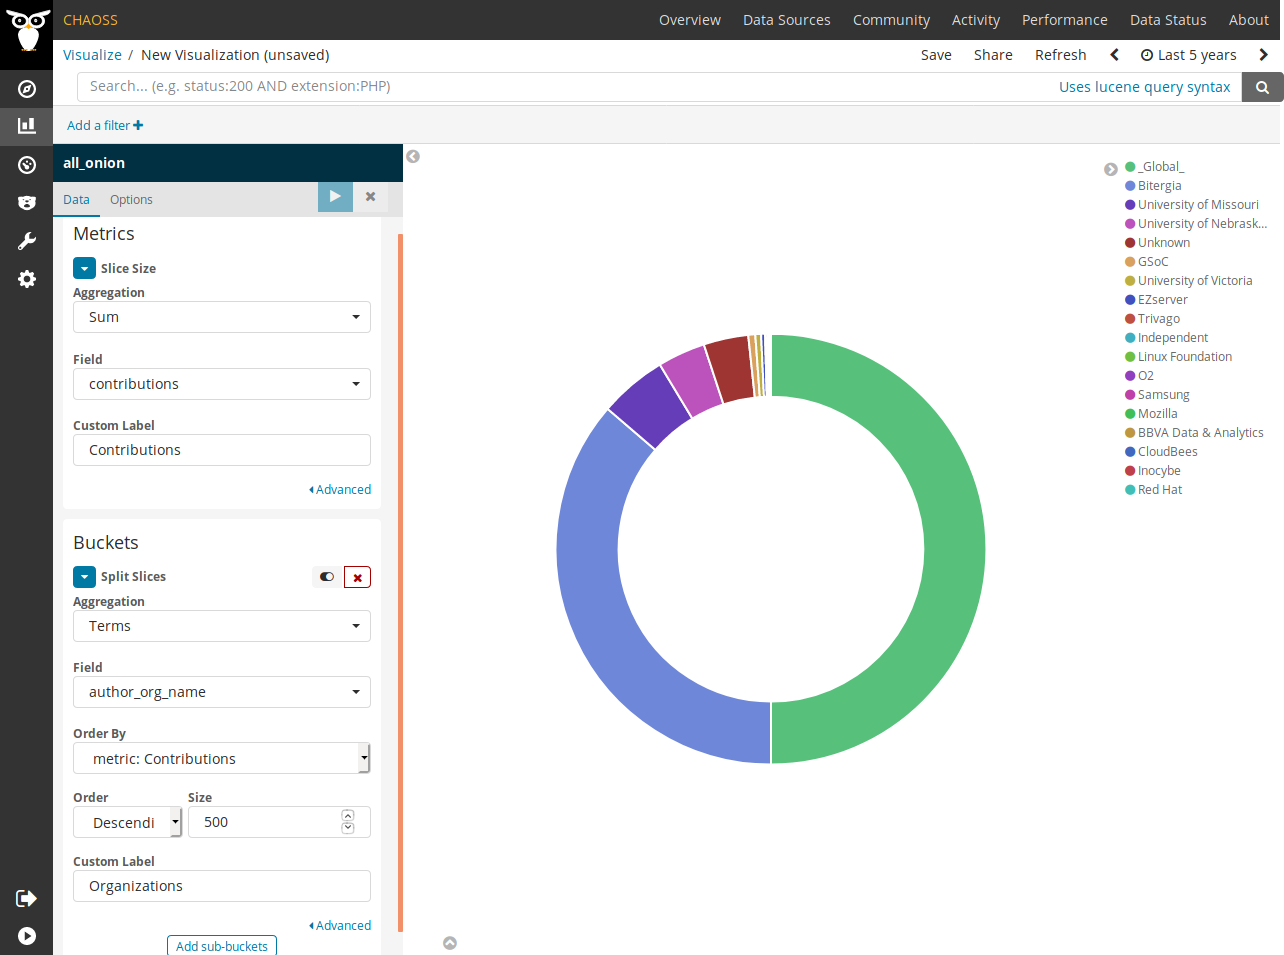
\includegraphics{images/organizational-diversity_piechart.png}
  \end{itemize}
\item
  \href{https://lfanalytics.io}{LF Analytics} provides organization
  diversity metrics in the primary view for commits, issues filed, and
  communication channels (current support for Slack and groups.io)
\end{itemize}

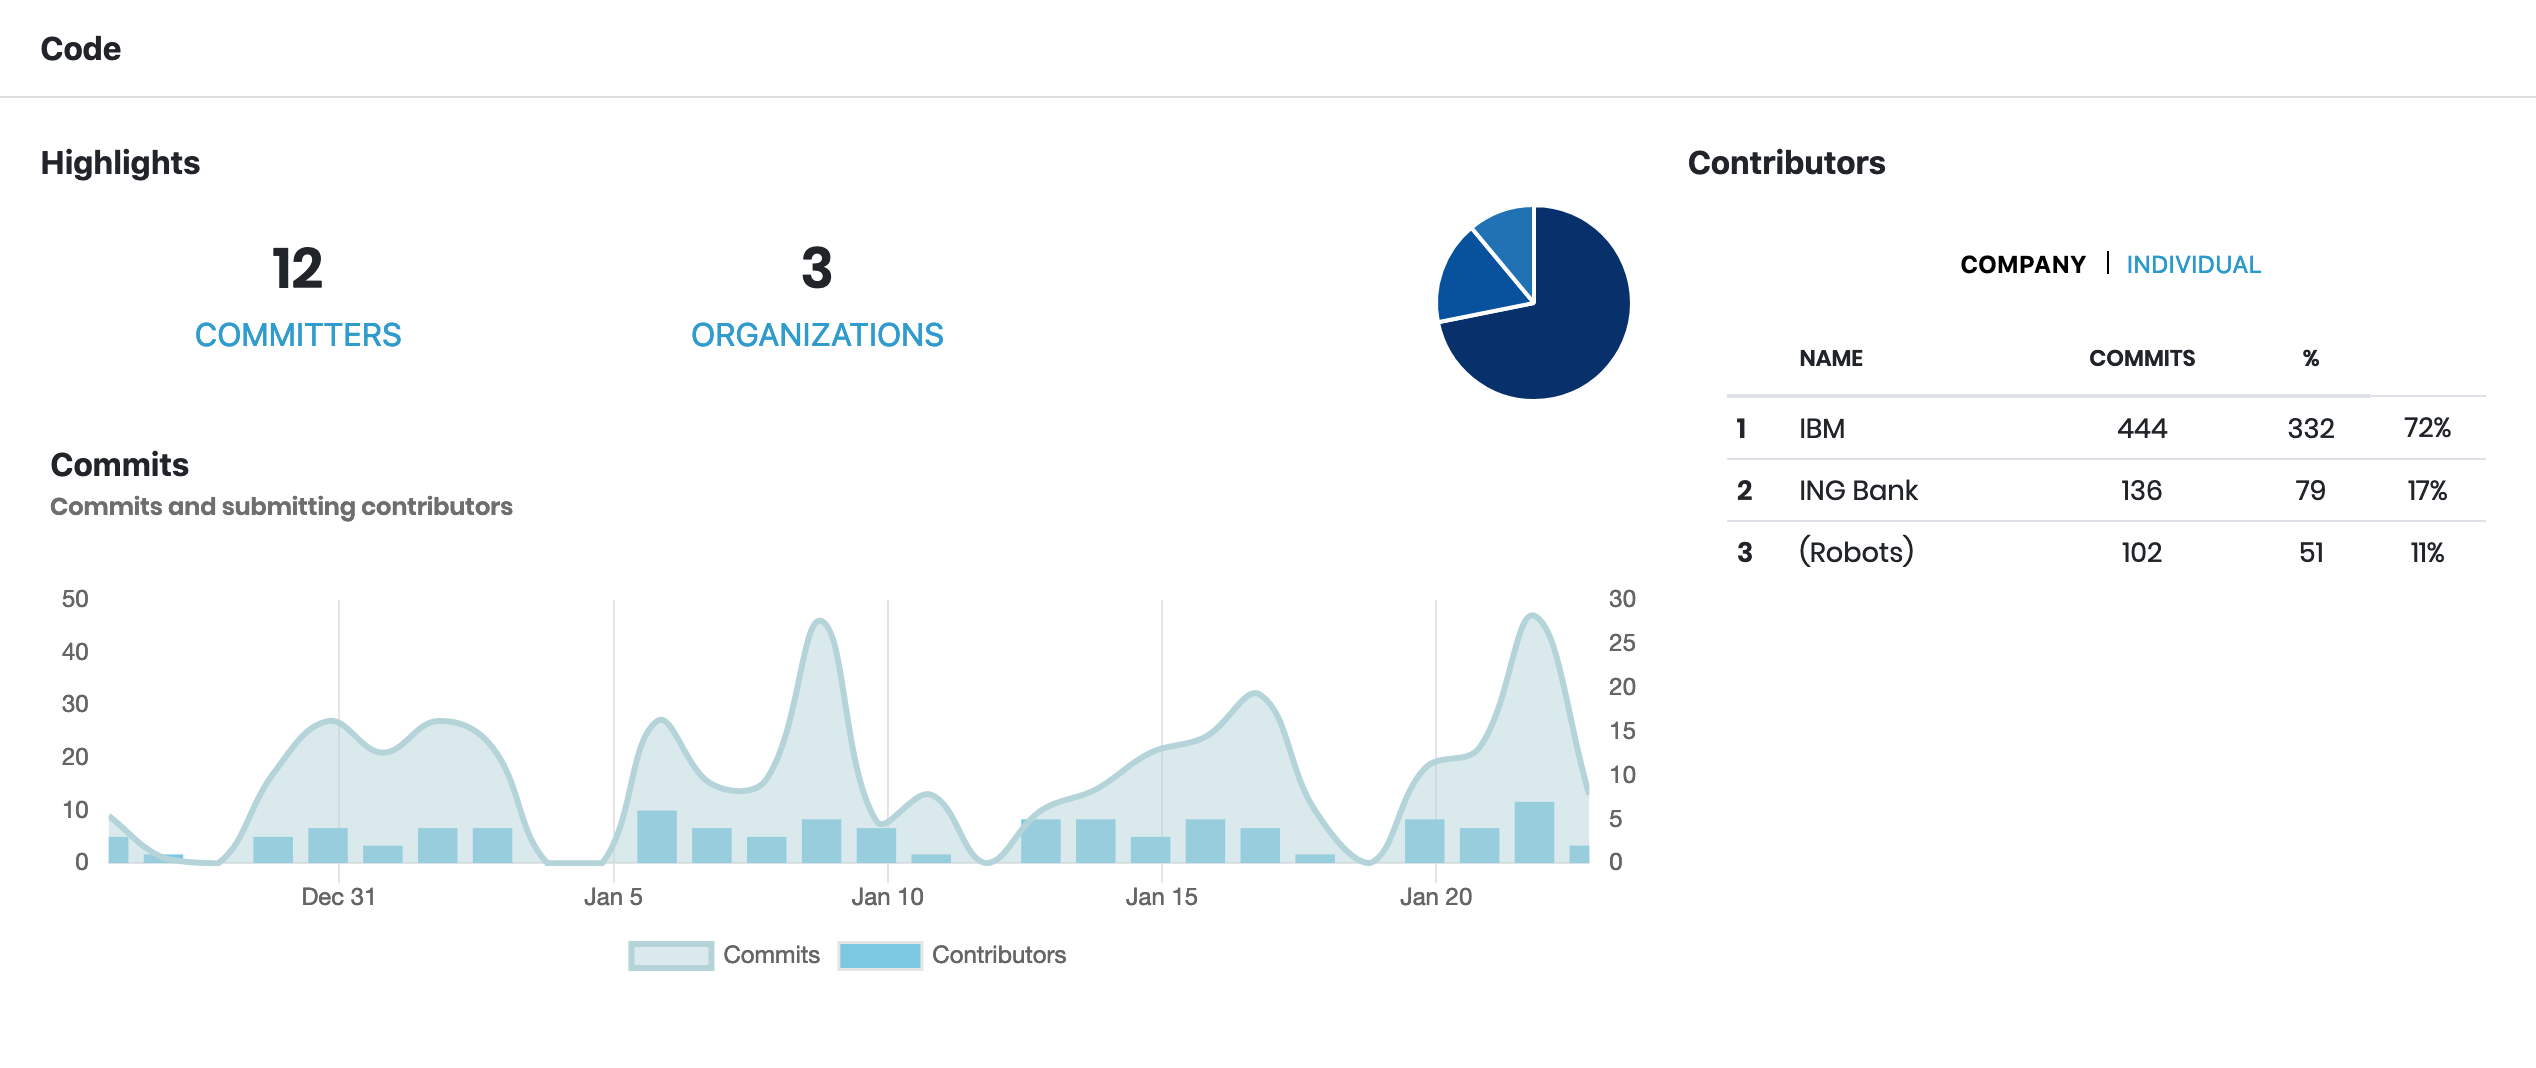
\includegraphics{images/organizational-diversity_lfanalytics-orgdiversity.png}

\hypertarget{data-collection-strategies}{%
\subsubsection{Data Collection
Strategies}\label{data-collection-strategies}}

\textbf{Qualitative}

\begin{itemize}
\tightlist
\item
  Footprint of an organization in a project or ecosystem
\item
  Influence of an organization in a project or ecosystem
\item
  Affiliation diversity in governance structures.
\end{itemize}

\textbf{Quantitative}

\begin{itemize}
\tightlist
\item
  \% of commits by each organization
\item
  \% of merges/reviews from each organization
\item
  \% of any kind of contributors from each organization
\item
  \% of lines of code contributed by each organization
\item
  \% issues filed by each organization
\item
  \href{https://github.com/chaoss/metrics/blob/master/activity-metrics/contributing-organizations.md}{Contributing
  Organizations} - What is the number of contributing organizations?
\item
  \href{https://github.com/chaoss/metrics/blob/master/activity-metrics/new-contributing-organizations.md}{New
  Contributing Organizations} - What is the number of new contributing
  organizations?
\item
  New Contributor Organizations - New organizations contributing to the
  project over time.
\item
  Number of Contributing Organizations - Number of organizations
  participating in the project over time.
\item
  Elephant Factor - If 50\% of community members are employed by the
  same company, it is the elephant in the room. Formally: The minimum
  number of companies whose employees perform 50\% of the commits
\item
  \href{https://github.com/chaoss/metrics/blob/master/activity-metrics/contributor-diversity.md}{Affiliation
  Diversity} - Ratio of contributors from a single company over all
  contributors. Also described as: Maintainers from different companies.
  Diversity of contributor affiliation.
\item
  In projects with the concept of code ownership, \% of code owners
  affiliated with each organization weighed by the importance/size/LoC
  of the code they own and the number of co-owners.
\end{itemize}

\hypertarget{references}{%
\subsection{References}\label{references}}

\begin{itemize}
\tightlist
\item
  Potential implementations and references:

  \begin{itemize}
  \tightlist
  \item
    \url{https://bitergia.gitlab.io/panel-collections/open_source_program_office/organizational-diversity.html}
  \item
    \href{https://katacontainers.biterg.io}{Kata Containers dashboard
    entry page} (bottom of this)
  \item
    \href{https://github.com/chaoss/augur}{Augur}
  \end{itemize}
\end{itemize}
 
 
 


\hypertarget{project-popularity}{%
\section{Project Popularity}\label{project-popularity}}

Question: How popular is an open source project?

\hypertarget{description}{%
\subsection{Description}\label{description}}

Project popularity can be measured by how much activity is visible
around a project. Popularity has a positive feedback loop in which more
popular projects get more attention, attract more users or developers,
and see increases in popularity, spinning the popularity wheel.

Project popularity may be used as a proxy for understanding project
value because open source project economic value is hard to measure, due
to a lack of available usage or sales information for open source
projects.

\hypertarget{objectives}{%
\subsection{Objectives}\label{objectives}}

In a quest to earn a living wage, and to maximize future employment
opportunities, workers may be interested in knowing which projects are
growing and are underserved. Similarly, from an organizational
perspective, knowing which projects are highly used can be helpful in
knowing which projects might be worth investing in. The Project
Popularity metric can be used to identify the trajectory of a project's
development.

\hypertarget{implementation}{%
\subsection{Implementation}\label{implementation}}

The project popularity metric is often considered with changes over
time. There are numerous example vectors to consider when measuring
project popularity based on the number of:

\begin{enumerate}
\def\labelenumi{\arabic{enumi}.}
\tightlist
\item
  Social media mentions
\item
  Forks
\item
  \href{https://chaoss.community/metric-change-requests/}{Change
  requests}
\item
  \href{https://chaoss.community/metric-issues-new/}{New Issues}
\item
  Stars, badges, likes
\item
  \href{https://chaoss.community/metric-new-contributors/}{New
  contributors}
\item
  \href{https://chaoss.community/metric-organizational-diversity/}{Organizational
  Diversity}
\item
  Job postings requesting skills in project
\item
  Conversations within and outside of project
\item
  Clones
\item
  Followers
\item
  Downstream dependencies
\item
  People attending events that focus on a project
\end{enumerate}

\hypertarget{visualizations}{%
\subsubsection{Visualizations}\label{visualizations}}

Issues and reviews (change requests) visualization from Cauldron
(GrimoireLab):

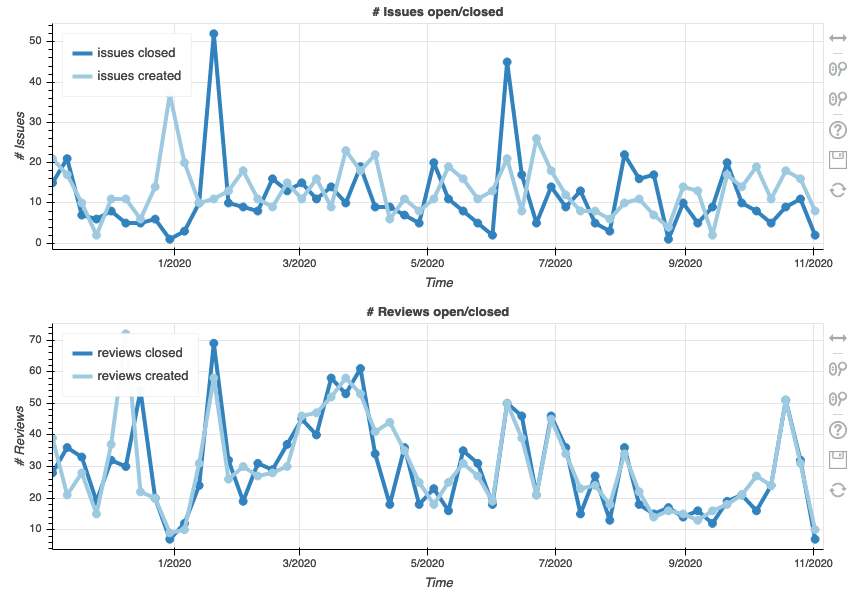
\includegraphics{images/project-popularity_issues-and-reviews.png}

Kubernetes project popularity statistics from DevStats:

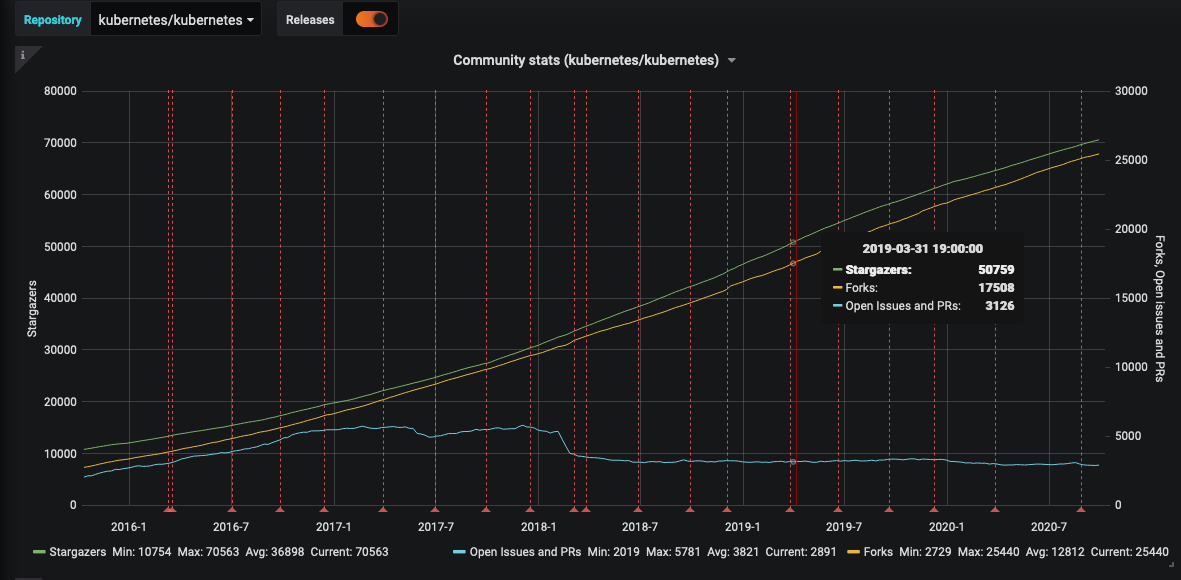
\includegraphics{images/project-popularity_kubernetes.png}

\hypertarget{tools-providing-the-metric}{%
\subsubsection{Tools Providing the
Metric}\label{tools-providing-the-metric}}

\begin{itemize}
\tightlist
\item
  \href{https://github.com/chaoss/augur}{Augur}
\item
  \href{https://chaoss.github.io/grimoirelab/}{GrimoireLab}
\item
  \href{https://cauldron.io/}{Cauldron}
\end{itemize}

\hypertarget{references}{%
\subsection{References}\label{references}}

\begin{itemize}
\tightlist
\item
  \href{http://blog.honeypot.io/most-exciting-open-source-projects-2018/}{Popular
  OpenSource Projects}
\item
  \href{https://isitmaintained.com/}{Is It Maintained?}
\item
  \href{https://github.blog/2018-02-08-open-source-project-trends-for-2018/}{Open
  Source Project Trends}
\item
  \href{https://www.payscale.com/research/US/Skill=Kubernetes/Salary}{Kubernetes
  Salary}
\end{itemize}
 
\hypertarget{project-velocity}{%
\section{Project Velocity}\label{project-velocity}}

Question: What is the development speed for an organization?

\hypertarget{description}{%
\subsection{Description}\label{description}}

Project velocity is the number of issues, the number of pull requests,
volume of commits, and number of contributors as an indicator of
'innovation'.

\hypertarget{objectives}{%
\subsection{Objectives}\label{objectives}}

Gives an Open Source Program Office (OSPO) manager a way to compare the
project velocity across a portfolio of projects.

The OSPO manager can use the Project Velocity metric to:

\begin{itemize}
\tightlist
\item
  Report project velocity of open source projects vs in-house projects
\item
  Compare project velocity across a portfolio of projects
\item
  Identify which projects grow beyond internal contributors (when
  filtering internal vs. external contributors)
\item
  Identify promising areas in which to get involved
\item
  Highlight areas likely to be the successful platforms over the next
  several years
\end{itemize}

\href{https://www.cncf.io/blog/2017/06/05/30-highest-velocity-open-source-projects}{See
Example}

\hypertarget{implementation}{%
\subsection{Implementation}\label{implementation}}

Base metrics include:

\begin{itemize}
\tightlist
\item
  \href{https://github.com/chaoss/wg-evolution/blob/master/metrics/Issues_Closed.md}{issues
  closed}
\item
  \href{https://github.com/chaoss/wg-evolution/blob/master/metrics/Reviews.md}{number
  of reviews}
\item
  \href{https://github.com/chaoss/wg-evolution/blob/master/metrics/Code_Changes.md}{\#
  of code changes}
\item
  \href{https://github.com/chaoss/wg-risk/blob/master/metrics/Committers.md}{\#
  of committers}
\end{itemize}

\hypertarget{filters}{%
\subsubsection{Filters}\label{filters}}

\begin{itemize}
\tightlist
\item
  Internal vs external contributors
\item
  Project sources (e.g., internal repositories, open-source
  repositories, and competitor open-source repositories)
\item
  Time
\end{itemize}

\hypertarget{visualizations}{%
\subsubsection{Visualizations}\label{visualizations}}

\begin{itemize}
\tightlist
\item
  X-Axis: Logarithmic scale for Code Changes
\item
  Y-Axis: Logarithmic scale of Sum of Number of Issues and Number of
  Reviews
\item
  Dot-size: Committers
\item
  Dots are projects
\end{itemize}

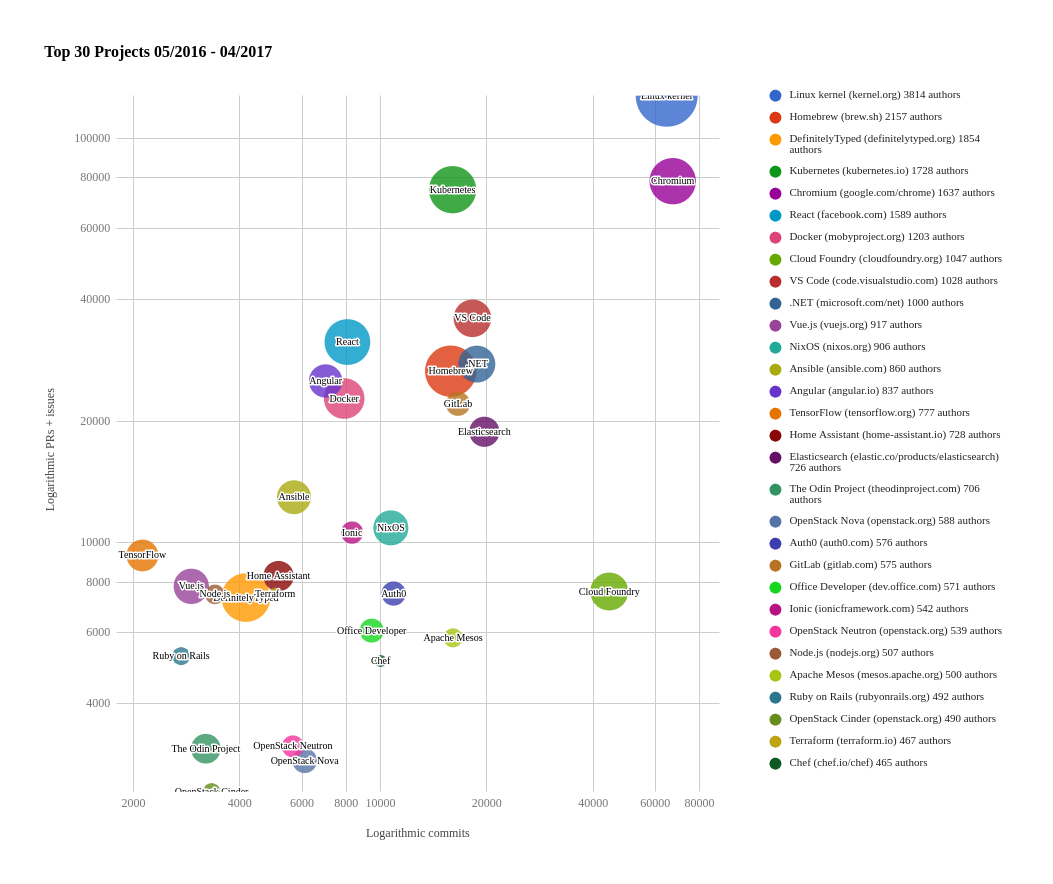
\includegraphics{images/project-velocity_visualization.png}

\href{https://www.cncf.io/blog/2017/06/05/30-highest-velocity-open-source-projects/}{From
CNCF}

\hypertarget{tools-providing-the-metric}{%
\subsubsection{Tools providing the
Metric}\label{tools-providing-the-metric}}

\begin{itemize}
\tightlist
\item
  CNCF - \url{https://github.com/cncf/velocity}
\end{itemize}

\hypertarget{references}{%
\subsection{References}\label{references}}

\begin{itemize}
\tightlist
\item
  \href{https://www.threefivetwo.com/blog/can-open-source-innovation-work-in-the-enterprise}{Can
  Open Source Innovation work in the Enterprise?}
\item
  \href{https://www.nearform.com/blog/want-a-high-performing-culture-make-way-for-open-innovation}{Open
  Innovation for a High Performance Culture}
\item
  \href{https://www.cio.com/article/3213146/open-source-is-powering-the-digital-enterprise.html}{Open
  Source for the Digital Enterprise}
\item
  \href{https://www.cncf.io/blog/2017/06/05/30-highest-velocity-open-source-projects}{Highest
  Velocity Open Source Projects}
\end{itemize}
 
\hypertarget{social-listening}{%
\subsubsection{Social Listening}\label{social-listening}}

Question: How does one measure the value of community interactions and
accurately gauge ``reputation'' of a community as evident from
qualitative sentiment?

\emph{Note: This metric synthesizes several other metrics that can be
derived from trace data, and several process-oriented metrics. Embedded
footnotes annotate areas planned for later clarification, and questions
for later resolution.}

\hypertarget{description}{%
\paragraph{Description}\label{description}}

Social Listening is a combination of
\href{https://blog.hubspot.com/service/social-listening}{social
listening} practices across multiple channels along with a meaningful
set of categorizations. The combination of these tactics can lead to
systematic community analysis and can inform a community strategy that
leads to measurable business value. 1

\textbf{Theory and Origin}

Social currency or social capital is a social scientific theory. It
broadly considers how human interactions build relationships and trust
in a community. The Social Listening metric represents the reputation of
a community as measured via community trust, transparency, utility,
consistency, and merit.

Interpersonal relationships are the social fabric of communities. This
is shown in the
\href{https://theadminzone.com/ams/levingers-stage-theory.1272/}{Levinger's
Relationship Model} and
\href{https://psycnet.apa.org/record/1973-28661-000}{Social Penetration
Theory}. Community members' sense of personal and group identity grows
as they interact. Members build shared values, accumulate a sense of
trust, encourage cooperation, and garner reciprocity through acts of
\href{https://en.wikipedia.org/wiki/Self-disclosure}{self-disclosure}.
These interactions build an increased and measurable sense of
connection. The measure of these characteristics is called social
currency. 2

\textbf{Results}

The Social Listening metric is a way to sort through a fire hose of
qualitative data from community interactions. A central premise of this
approach is that community members' interactions have an impact on the
community. The Social Listening metric continually measures the
sentiment 3 from those interactions. It illustrates the reputation and
level of trust between community members and leaders. 4

\hypertarget{objectives}{%
\paragraph{Objectives}\label{objectives}}

Analyze the qualitative comments in community interactions. Gain an
overview of sentiment in a community. Get metrics that show at a glance
how a community is and was doing. Use lead metrics from continuous
measurements for proactive community strategy development. Instill trust
in community members that their thoughts and opinions are valued.

\hypertarget{implementation}{%
\paragraph{Implementation}\label{implementation}}

The Social Listening requires the collection of community comments
(communication traces), the definition of a codex, and the on-going
review of the communication traces. 5

Set up a Data Collection Platform of your choice as described in the
``Tools'' section below. Ensure it has a minimum of 4 dimensions and 3
communication channels. Once it is set up, the following method is used
to collect, analyze, and interpret results:


\includegraphics{images/social-listening_circle2.png}

\begin{enumerate}
\def\labelenumi{\arabic{enumi}.}
\item
  \textbf{Collect Communication Traces} -\/- Identify online platforms
  that your community is communicating on. Set up data funnels from the
  primary platform to your Social Listening tool. The critical data for
  the system is user generated content.
\item
  \textbf{Standardize How Communication Traces Should Be Assessed} -\/-
  Use a codex to define important concepts as a ``tracking keyword'' or
  ``category'' in the focal community. This unified codex of terms
  ensures consistent analysis as different people read and tag community
  sentiment. Formalizing the revision and addition structure to this
  codex on a regular basis is a must. 5
\item
  \textbf{Analyze the Communication Traces} -\/- Community sentiment is
  analyzed in the Social Listening tool by tagging data with codex
  terms. If the tagging is done by a team of people, it is recommended
  that everyone gets together regularly to discuss trends and ensure
  consistent tag use. If the tagging is done by an artificial
  intelligence algorithm, then a human team should supervise and retrain
  the AI as necessary. 5
\item
  \textbf{Share and Visualize the Aggregated Analysis} -\/- Visualize
  the quantitative count of codex terms over time, e.g., in a dashboard.
  This is where the qualitative analysis results produce an easy to
  observe dashboard of trends. Share analysis with team members. 6
\item
  \textbf{Benchmark, Set Goals \& Predict Future Growth} -\/- After
  getting enough data to form a benchmark, take stock of where your
  community stands. What are its strengths and weaknesses? What actions
  can be taken to make the community healthier and more robust? Then
  form community initiatives with well-defined goals and execute on
  these projects to affect the social currency metrics for next week. 6
\item
  \textbf{Repeat the Process} -\/- In regular evaluation meetings,
  discuss the shortcomings of the dataset or collection methods. Come up
  with methods to address these shortcomings in the future. Work
  solutions into the system and move forward. Truth is in the trend,
  power is in the pattern.7
\end{enumerate}

\hypertarget{filters}{%
\subparagraph{Filters}\label{filters}}

\begin{enumerate}
\def\labelenumi{\arabic{enumi}.}
\tightlist
\item
  \textbf{Channel}: Sort by where the data was collected from.
\item
  \textbf{Tag}: Show data based on what codex tags were used to identify
  sentiment in comments.
\item
  \textbf{Time}: Show trends in the data over time and pull specific
  data-sets.
\item
  \textbf{Most impactful comments}: Sort and filter by flags that can be
  placed in the data to highlight specific data points and explain their
  importance.
\item
  \textbf{AI vs. Human tagged}: Filter by whether tags were applied
  programmatically or by a person.
\item
  \textbf{Weighted currency:} Weight the ``importance'' of certain
  comments based on any one individually selected criteria. A resulting
  weighted view is simply a re-order of information based on weight.
\end{enumerate}

\hypertarget{visualizations}{%
\subparagraph{Visualizations}\label{visualizations}}

\textbf{Dashboard visualizing the aggregate metrics:}

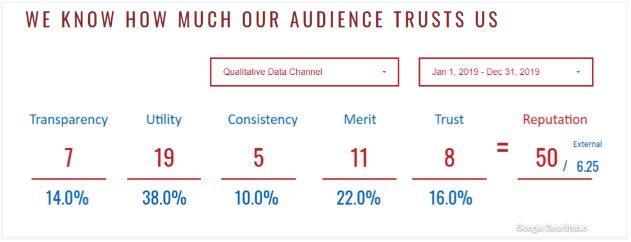
\includegraphics{images/social-listening_dashboard.png}

\textbf{Example Social Listening tool:} On the left, raw community
comments are shown and tags are added in columns immediately to the
right. On the right, a pivot table shows in numbers how often tags
occurred in combination with other tags.

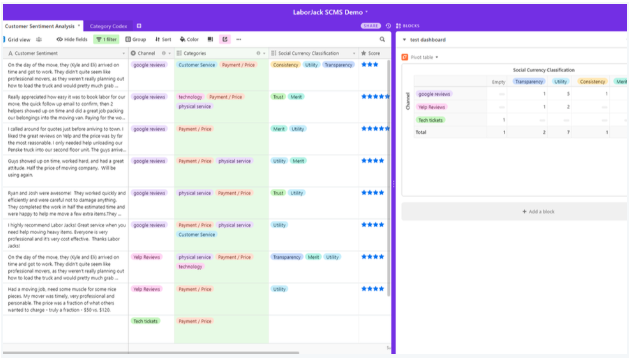
\includegraphics{images/social-listening_tool-example.png}

\textbf{Expanded comments view:} remove the ``quantitative'' from the
fields and provide the best possible way to read the different comments.

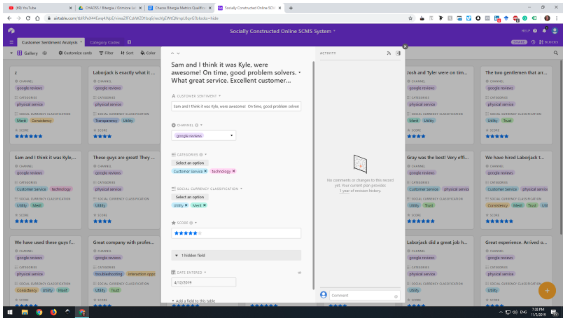
\includegraphics{images/social-listening_expanded-comment.png}

\hypertarget{tools-providing-the-metric}{%
\subparagraph{Tools Providing the
Metric}\label{tools-providing-the-metric}}

To implement the metric any MySQL, smart-sheet, excel, or airtable-like
excel datasheet program works fine. This data should be simplified
enough to interact with other data interfaces to ensure that data
migration is simple, straightforward, and can be automated (such as
google data studio). This requires that systems used to implement the
Social Listening metric work with CSV and other spreadsheet files, and
we heavily recommend open source programs for its implementation.

Once you have this, create a data set with the following data points: 8

\begin{longtable}[]{@{}ll@{}}
\toprule
Data Points & Description \\
\midrule
\endhead
Date of entry & Date data was imported to Social Listening tool \\
Date of comment & Date comment was made on original platform \\
Comment Text & Qualitative data brought in. Decide on how large you want
these chunks ported. Some may port an entire email while others will be
broken into one row per sentence. It should only have one
``sentiment'' \\
Data channel & Originating data channel the comment came from \\
Tags (created on codex document below) & Based on the unified codex of
terms, decide what tags to track. There can be two kinds of tags. On the
one hand, tags can be based on ``themes'' or recurring sentiment that
people voice (e.g., gamer gate, flamewar, or thank you notes). On the
other hand, tags based on ``categories'' can describe different aspects
of a community that members comment on (e.g., events, release, or
governance). \\
Social Currency Metric & The social currency being awarded or demerited
in the system. This will directly affect numbers. \\
Weighted Score & Once you've decided what your ``weight'' will be, you
can assign a system of -3 to +3 to provide a weighted view of
human-tagged metrics (AI will not assign a weight for several reasons).
This enables the ``most impactful comment'' filter. \\
\bottomrule
\end{longtable}

Create a second sheet for the Unified Codex of Terms which will define
terms. It should look like this: 8

\begin{longtable}[]{@{}llll@{}}
\toprule
Category Term & Definition & When to use & When not~to use \\
\midrule
\endhead
{[}Custom Tags - themes and categories{]} & & & \\
{[}Community specific jargon{]} & & & \\
Social Currency Dimensions: & & & \\
TRANSPARENCY & Do people recognize and feel a connection to your
community?~ & When they have the "words" to pinpoint why they feel you
are authentic or personable. & This is not about good customer service,
or doing well. That is utility. This is about whether they understand
who you are as a business and show they are onboard with it. \\
UTILITY & Is your community doing something useful or is it contributing
value? & Provide parameters that exclude when the term is used so that
people know when the category tag should not be implemented. & This is
not about good customer service, or doing well. That is utility. This is
about whether they understand who you are as a business and show they
are onboard with it. \\
CONSISTENCY & Do you have a history of being reliable and dependable? &
When they suggest they have used your brand, or interacted with you
several times & If they've only provided their comment to suggest you
were useful once, use utility instead. \\
MERIT & Does your community merit respect and attention for your
accomplishments? & When the social currency garnered from customers
seems it will continue for a while, and will impact other people's
opinions. & When they suggest they will use you again in the future use
trust instead as that is a personal trust in the brand. Merit is
external. \\
TRUST & Can people trust that your community will continue to provide
value and grow in the future? & When they suggest they trust you well
enough to continue conversations with you in the future & When there is
not substantial enough evidence to suggest they will continue to work
with and trust you as a loyal customer or community member. \\
INTERNAL REPUTATION 9 & Do people believe these things strongly enough
to warrant conversation or action? & & \\
EXTERNAL REPUTATION 9 & What amount of your reputation in your community
is transferable to strangers outside of your community (cold audiences)?
& & \\
\bottomrule
\end{longtable}

The codex is filled in by stakeholders on a regular basis by specific
communities and forms the basis for analysis of the data. This is the
MOST IMPORTANT part. Without this the subjectivity of qualitative data
does not follow the rule of generalization: 9

\begin{quote}
``A concept applies to B population ONLY SO FAR AS C limitation.''
\end{quote}

\hypertarget{data-collection-strategies}{%
\subparagraph{Data Collection
Strategies}\label{data-collection-strategies}}

Community member comments are available from trace data. The Social
Listening metric ideally imports the comment text automatically into a
tool for tagging. Trace data can be collected from a communities'
collaboration platforms where members write comments, including
ticketing systems, code reviews, email lists, instant messaging, social
media, and fora.

\textbf{Legal and Regulatory Considerations}

\emph{Points of destruction}: Detailed data is destroyed after \emph{xx}
months has passed. Quantitative calculations are kept for up to 250
weeks per GDPR compliance. Data older than 250 weeks becomes archived
data you cannot manipulate but can see. Users can negotiate the primary
statistic.

\hypertarget{references}{%
\paragraph{References}\label{references}}

\begin{itemize}
\tightlist
\item
  \href{https://airtable.com/invite/l?inviteId=inv8u49VVMtQTrfFU\&inviteToken=c49b1ed3759c5cd736901fd81c9f460f86e8e9f462703c4f85a3bdd7250ca5a7}{An
  example implementation on airtable}
\item
  \href{https://datastudio.google.com/open/1X9UdQz8FtHHmjMBpjba3pFqE55lNpwg5}{An
  example implementation in data studio}(report)
\item
  \href{https://datastudio.google.com/open/1Z4EJ03898lZxm2NZVULaEoLS0bYqL79A}{An
  example implementation in data studio} (data source)
\item
  \href{https://drive.google.com/open?id=1zi3JE0bwfEdRdc-wQEZn8GaB7sE8IvxeSeqvVywKnXw}{An
  example implementation in google sheets}
\item
  \href{https://docs.google.com/document/d/1RlAedRBQbhq0oYMCB3VqdawOCZE2XT5R3teydjBZODM/edit\#heading=h.8hyunaadfriq}{Implementation
  documentation} (starts on page 33)
\end{itemize}

\hypertarget{annotated-footnotes}{%
\paragraph{Annotated Footnotes}\label{annotated-footnotes}}

1 CHAOSS metrics historically is to create standard definitions that can
be used reliably across projects to support comparisons. This metric may
evolve into a project in the future.

2 What metrics emerge from this description? Likely included are: 1.
community trust, 2. transparency, 3. utility, 4. consistency, and 5.
merit

3 Analysis of sentiment suggests that metric (6) is likely
"Communications Sentiment", and the definition may need to include
references to common sentiment analysis tools, sometimes called "bags of
words".

4 Measuring how trust trust is instilled in community members, such that
their thoughts and opinions are valued is likely metric (7) that will
define a process, and perhaps is not measurable via trace data.

5 A substantial portion of any codex for open source software will be
common across projects, and each project is likely to have a set of
particular interests that are a subset of that codex. In some cases,
their main interests may not be present in an established codex
component. In general, the codex, like the CHAOSS project itself, is
open sourced as shared metadata to ensure shared understanding across
open source communities.

6 This describes the evolution of a standard codex, and its elements
through the process of CHAOSS working groups and projects, characterized
in the previous footnote. Likely this will be a process metric (8).

7 Candidate process oriented metric (9).

8 Examples of data coded using the open sourced codex, as it evolves,
will be essential components for advancing open source software through
Social Listening. Implementations will require these examples, and their
provision as open source assets of the CHAOSS project will return value
as shared data.

9 Internal and external reputation are likely metrics (10), and (11)
arising from the Social Listening metric.
 
 

\hypertarget{job-opportunities}{%
\section{Job Opportunities}\label{job-opportunities}}

Question: How many job postings request skills with technologies from a
project?

\hypertarget{description}{%
\subsection{Description}\label{description}}

A common way for open source contributors to earn a living wage is to be
employed by a company or be a self-employed or freelance developer.
Skills in a specific project may improve a job applicant's prospects of
getting a job. The most obvious indicator for demand related to a skill
learned in a specific open source project is when that project or its
technology is included in job postings.

\hypertarget{objectives}{%
\subsection{Objectives}\label{objectives}}

The metric gives contributors a sense of how much skills learned in a
specific open source project are valued by companies.

\hypertarget{implementation}{%
\subsection{Implementation}\label{implementation}}

To obtain this metric on a job search platform (e.g., LinkedIn, Indeed,
or Dice), go to the job search and type in the name of the open source
project. The number of returned job postings is the metric. Periodically
collecting the metric through an API of a job search platform and
storing the results allows to see trends.

\hypertarget{filters}{%
\subsubsection{Filters}\label{filters}}

\begin{itemize}
\tightlist
\item
  Age of job posting; postings get stale and may not be removed when
  filled
\end{itemize}

\hypertarget{visualizations}{%
\subsubsection{Visualizations}\label{visualizations}}

The metric can be extended by looking at:

\begin{itemize}
\tightlist
\item
  Salary ranges for jobs returned
\item
  Level of seniority for jobs returned
\item
  Availability of jobs like on-site or off-site
\item
  Location of job
\item
  Geography
\end{itemize}

\hypertarget{references}{%
\subsection{References}\label{references}}

\begin{itemize}
\tightlist
\item
  LinkedIn Job Search API:
  \url{https://developer.linkedin.com/docs/v1/jobs/job-search-api\#}
\item
  Indeed Job Search API:
  \url{https://opensource.indeedeng.io/api-documentation/docs/job-search/}
\item
  Dice.com Job Search API:
  \url{http://www.dice.com/external/content/documentation/api.html}
\item
  Monster Job Search API: \url{https://partner.monster.com/job-search}
\item
  Ziprecruiter API (Requires Partnership):
  \url{https://www.ziprecruiter.com/zipsearch}
\end{itemize}

\emph{Note:} This metric is limited to individual projects but
engagement in open source can be beneficial for other reasons. This
metric could be tweaked to look beyond a single project and instead use
related skills such as programming languages, processes, open source
experience, or frameworks as search parameters for jobs.
 
\hypertarget{organizational-project-skill-demand}{%
\subsubsection{Organizational Project Skill
Demand}\label{organizational-project-skill-demand}}

Question: How many organizations are using this project and could hire
me if I become proficient?

\hypertarget{description}{%
\paragraph{Description}\label{description}}

Organizations engage with open source projects through use and
dependencies. This metric is aimed at determining downstream demand of
skills related to an open source project. This metric looks at
organizations that deploy a project as part of an IT infrastructure,
other open source projects with declared dependencies, and references to
the project through social media, conference mentions, blog posts, and
similar activities.

\hypertarget{objectives}{%
\paragraph{Objectives}\label{objectives}}

As a developer, I'd like to invest my skills and time in a project that
has a likelihood of getting me a decent paying job in the future. People
can use the Downstream Organizational Impact of a Project Software
metric to discover which projects are used by organizations, and they
may, therefore, be able to pursue job opportunities with, possibly
requiring IT support services.

\hypertarget{implementation}{%
\paragraph{Implementation}\label{implementation}}

Base metrics include:

\begin{itemize}
\tightlist
\item
  Number of organizations that created issues for a project
\item
  Number of organizations that created pull requests for a project
\item
  Number of organizations that blog or tweet about a project
\item
  Number of organizations that mention a project in open hiring requests
\item
  Number of organizations that are represented at meetups about this
  project
\item
  Number of other projects that are dependent on a project
\item
  Number of books about a project
\item
  Google search trends for a project
\end{itemize}

\hypertarget{visualizations}{%
\subparagraph{Visualizations}\label{visualizations}}

The following visualization demonstrates the number of downstream
projects dependendent on the project in question. While this
visualization does not capture the entirety of the Downstream
Organizational Impact of a Project Software metric, it provides a visual
for a portion.

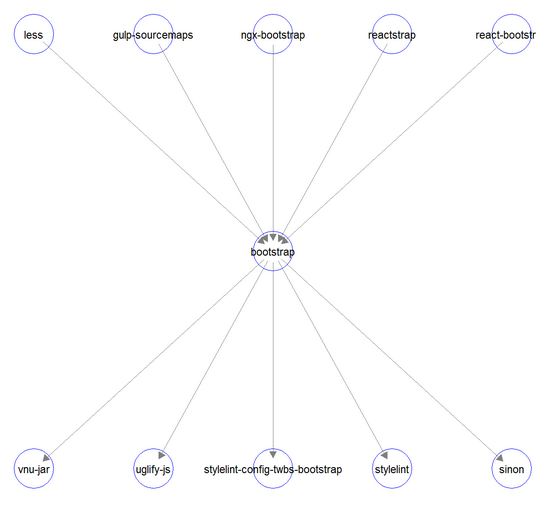
\includegraphics{images/organizational-project-skill-demand_paper.png}

Other visualizations could include Google search trends (React vs.
Angular vs. Vue.js)

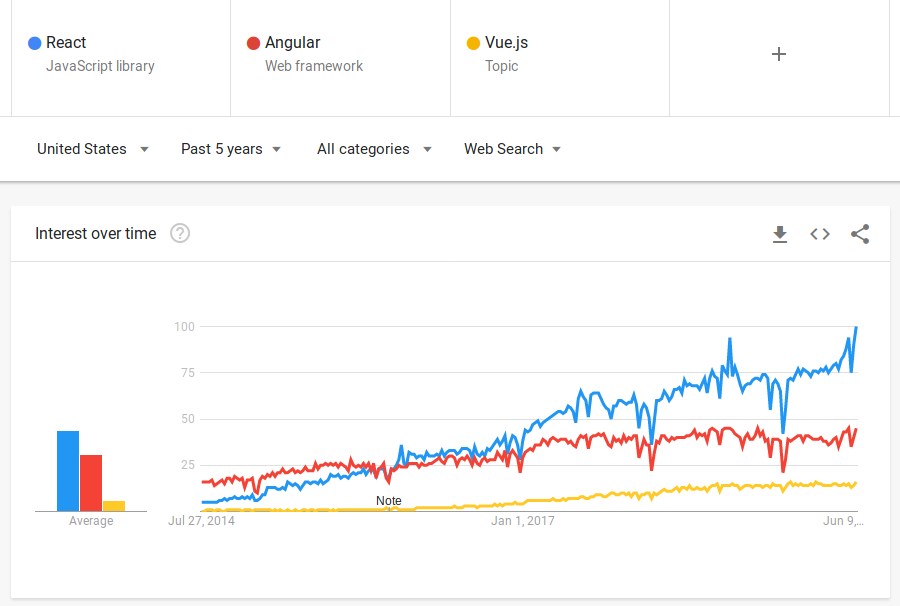
\includegraphics{images/organizational-project-skill-demand_google-trends.png}

ThoughtWorks publishes a series called 'Tech Radar' that shows the
popularity of technologies.

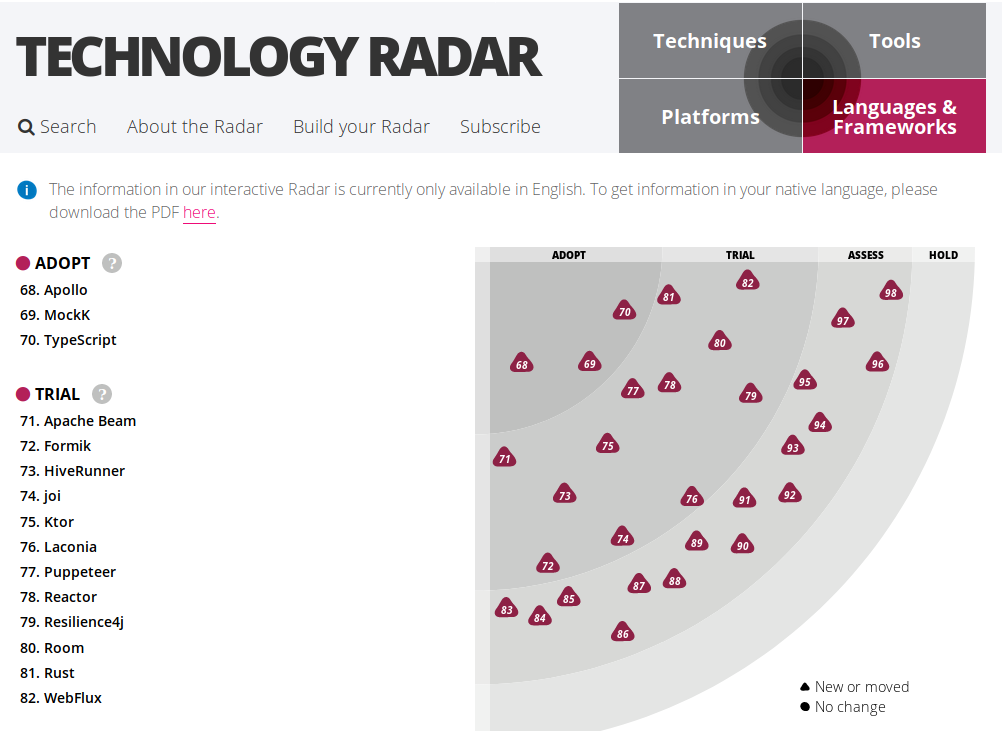
\includegraphics{images/organizational-project-skill-demand_tech-radar.png}

Tech Radar allows you to drill down on projects to see how the
assessment has changed over time.

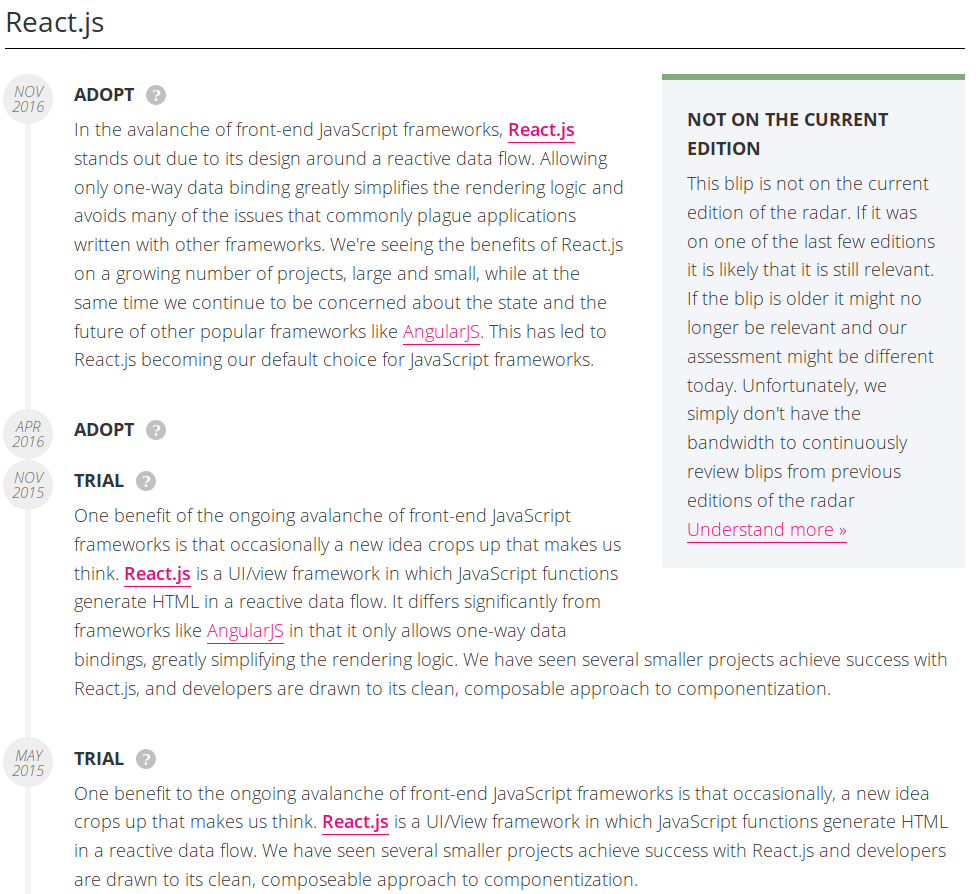
\includegraphics{images/organizational-project-skill-demand_tech-react.png}

StackOverview publishes an annual developer's survey

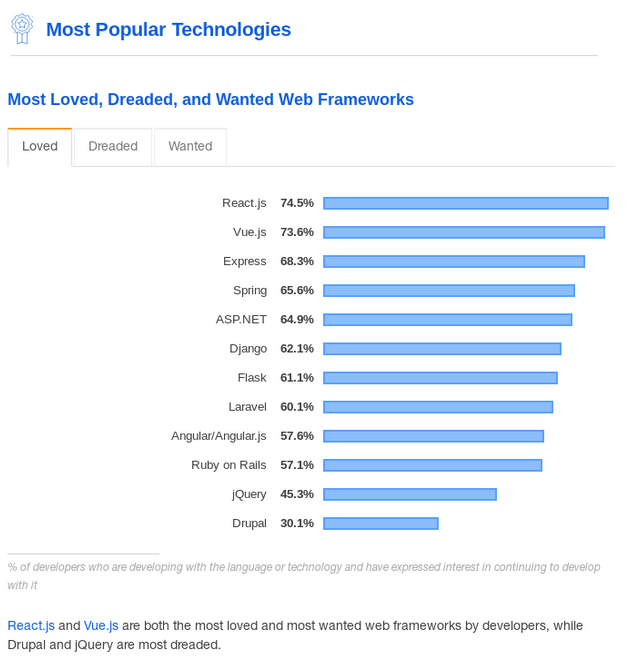
\includegraphics{images/organizational-project-skill-demand_stack-overflow.png}

\hypertarget{tools-providing-the-metric}{%
\subparagraph{Tools Providing the
Metric}\label{tools-providing-the-metric}}

\begin{itemize}
\tightlist
\item
  Google Trends - for showing search interest over time
\item
  ThoughtWorks TechRadar - project assessments from a tech consultancy
\item
  StackOverflow Developer's Survey - annual project rankings
\item
  Augur; Examples are available for multiple repositories:

  \begin{itemize}
  \tightlist
  \item
    \href{http://augur.osshealth.io/repo/Rails\%20(wg-value)/rails/overview}{Rails}
  \item
    \href{http://augur.osshealth.io/repo/Zephyr-RTOS/zephyr/overview}{Zephyr}
  \item
    \href{http://augur.osshealth.io/repo/Apache\%20(wg-value)/cloudstack/overview}{CloudStack}
  \end{itemize}
\end{itemize}

\hypertarget{references}{%
\paragraph{References}\label{references}}

\begin{itemize}
\tightlist
\item
  \href{https://opensource.org/sponsors}{Open Source Sponsors}
\item
  \href{https://opensource.com/article/19/1/fiscal-sponsors-open-source}{Fiscal
  Sponsors and Open Source}
\item
  \href{https://www.networkworld.com/article/2867020/big-names-like-google-dominate-open-source-funding.html}{Large
  Corporate OpenSource Sponsors}
\item
  \href{https://www.npmjs.com/package/google-trends-api}{Google Trends
  API}
\item
  \href{https://aisel.aisnet.org/cgi/viewcontent.cgi?article=1496\&context=amcis2018}{Measuring
  Open Source Software Impact}
\item
  \href{https://www.thoughtworks.com/radar}{ThoughtWorks Tech Radar}
\item
  \href{https://insights.stackoverflow.com/survey/2019\#technology}{Stack
  Overflow Developer's Survey}
\end{itemize}
 
 
 

\end{document}


\subsection{Focus Area - What}
\textbf{Goal:} 
\begin{table}[ht!]
    \centering
    \begin{tabular}{|p{0.35\linewidth} | p{0.6\linewidth}|}
        \hline
        \hfil \textbf{Metric}  & \hfil \textbf{Question} \\
        \hline
		Technical Fork & What are a number of technical forks of an open source project on code development platforms? \\ 
		\hline
		Types of Contributions & What types of contributions are being made? \\ 
		\hline
    \end{tabular}
\end{table}

\hypertarget{technical-fork}{%
\section{Technical Fork}\label{technical-fork}}

Question: What are a number of technical forks of an open source project
on code development platforms?

\hypertarget{description}{%
\subsection{Description}\label{description}}

A technical fork is a distributed version control copy of a project. The
number of technical forks indicates the number of copies of a project on
the same code development platform.

\hypertarget{objectives}{%
\subsection{Objectives}\label{objectives}}

The objective of the Technical Fork metric is to ascertain how many
copies of a project exist on a code development platform. Analysis of
technical forks may provide insight into forking intentions (different
types of forks such as contributing, and non-contributing forks).

\hypertarget{implementation}{%
\subsection{Implementation}\label{implementation}}

\hypertarget{filters}{%
\subsubsection{Filters}\label{filters}}

\begin{itemize}
\tightlist
\item
  Time Period (e.g., Weekly, Monthly, Annually)
\item
  Ratio of contributing fork to total forks (A contributing fork is a
  fork that has opened a change request against the original
  repository.)
\item
  Ratio of non-contributing fork to total forks (A non-contributing fork
  is a fork that has never opened a change request against the original
  repository.)
\end{itemize}

\hypertarget{visualizations}{%
\subsubsection{Visualizations}\label{visualizations}}

\textbf{Augur Implementation}\\
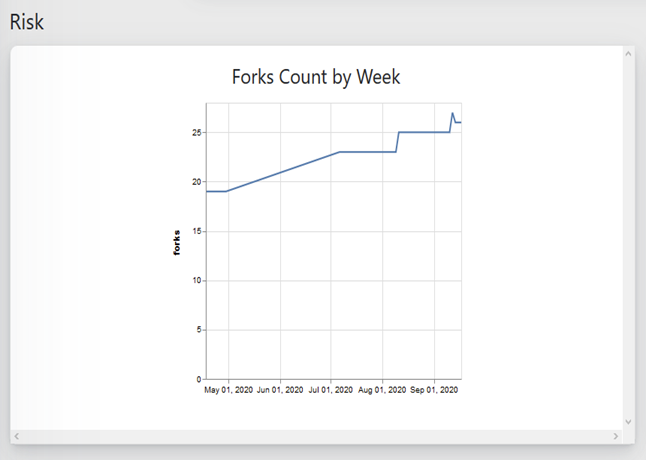
\includegraphics{images/technical-fork_augur-fork.png}

\textbf{GrimoireLab Implementation}\\
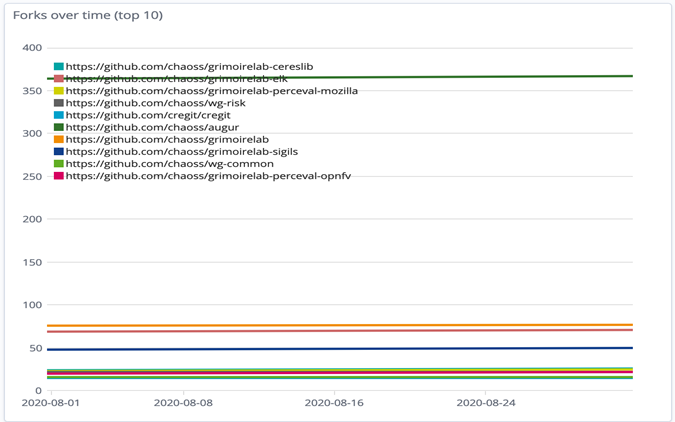
\includegraphics{images/technical-fork_grimoirelab-fork.png}

\hypertarget{tools-providing-the-metric}{%
\subsubsection{Tools Providing the
Metric}\label{tools-providing-the-metric}}

\begin{itemize}
\tightlist
\item
  Augur
\item
  GrimoireLab
\end{itemize}

\hypertarget{data-collection-strategies}{%
\subsubsection{Data Collection
Strategies}\label{data-collection-strategies}}

\textbf{Github API}\\
\url{https://developer.github.com/v3/repos/forks/\#list-forks}

\textbf{GitLab API}\\
\url{https://docs.gitlab.com/ee/api/projects.html\#list-forks-of-a-project}

\textbf{Bitbucket API}\\
\url{https://developer.atlassian.com/bitbucket/api/2/reference/resource/repositories/\%7Bworkspace\%7D/\%7Brepo_slug\%7D/forks}

\hypertarget{references}{%
\subsection{References}\label{references}}

\url{https://help.github.com/en/enterprise/2.13/user/articles/fork-a-repo}
\url{https://opensource.com/article/17/12/fork-clone-difference}
 
\hypertarget{types-of-contributions}{%
\section{Types of Contributions}\label{types-of-contributions}}

Question: What types of contributions are being made?

\hypertarget{description}{%
\subsection{Description}\label{description}}

Multiple, varied contributions make an open source project healthy. Many
projects have community members who do not write code but contribute in
equally valuable ways by managing the community, triaging bugs,
evangelizing the project, supporting users, or helping in other ways.

\hypertarget{objectives}{%
\subsection{Objectives}\label{objectives}}

A variety of contribution types can demonstrate that a project is mature
and well-rounded with sufficient activity to support all aspects of the
project, and enable paths to leadership that are supportive of a variety
of contribution types and people with varying expertise beyond coding.

\hypertarget{implementation}{%
\subsection{Implementation}\label{implementation}}

How contributions are defined, quantified, tracked and made public is a
challenging question. Answers may be unique to each project and the
following suggestions are a starting point. As a general guideline, it
is difficult to compare different contribution types with each other and
they might better be recognized independently.

\begin{itemize}
\tightlist
\item
  The following list can help with identifying contribution types:

  \begin{itemize}
  \tightlist
  \item
    Writing Code
  \item
    Reviewing Code
  \item
    Bug Triaging
  \item
    Quality Assurance and Testing
  \item
    Security-Related Activities
  \item
    Localization/L10N and Translation
  \item
    Event Organization
  \item
    Documentation Authorship
  \item
    Community Building and Management
  \item
    Teaching and Tutorial Building
  \item
    Troubleshooting and Support
  \item
    Creative Work and Design
  \item
    User Interface, User Experience, and Accessibility
  \item
    Social Media Management
  \item
    User Support and Answering Questions
  \item
    Writing Articles
  \item
    Public Relations - Interviews with Technical Press
  \item
    Speaking at Events
  \item
    Marketing and Campaign Advocacy
  \item
    Website Development
  \item
    Legal Council
  \item
    Financial Management
  \end{itemize}
\end{itemize}

\hypertarget{data-collection-strategies}{%
\subsubsection{Data Collection
Strategies}\label{data-collection-strategies}}

\begin{itemize}
\tightlist
\item
  \textbf{Interview or Survey:} Ask community members to recognize
  others for their contributions to recognize contribution types that
  have previously not been considered.

  \begin{itemize}
  \tightlist
  \item
    Who in the project would you like to recognize for their
    contributions? What did they contribute?
  \end{itemize}
\item
  \textbf{Observe project:} Identify and recognize leads of different
  parts of the project.

  \begin{itemize}
  \tightlist
  \item
    What leaders are listed on the project website or in a repository?
  \end{itemize}
\item
  \textbf{Capture Non-code Contributions:} Track contributions through a
  dedicated system, e.g., an issue tracker.

  \begin{itemize}
  \tightlist
  \item
    Logging can include custom information a project wants to know about
    non-code contributions to recognize efforts.
  \item
    Proxy contributions through communication channel activity. For
    example, If quality assurance members (QA) have their own mailing
    list, then activity around QA contributions can be measured by proxy
    from mailing list activity.
  \end{itemize}
\item
  \textbf{Collect Trace Data:} Measure contributions through
  collaboration tool log data.

  \begin{itemize}
  \tightlist
  \item
    For example, code contributions can be counted from a source code
    repository, wiki contributions can be counted from a wiki edit
    history, and email messages can be counted from an email archive
  \end{itemize}
\item
  \textbf{Automate Classification:} Train an artificial intelligence
  (AI) bot to detect and classify contributions.

  \begin{itemize}
  \tightlist
  \item
    An AI bot can assist in categorizing contributions, for example,
    help requests vs. support provided, or feature request vs. bug
    reporting, especially if these are all done in the same issue
    tracker.
  \end{itemize}
\end{itemize}

\emph{Other considerations:}

\begin{itemize}
\tightlist
\item
  Especially with automated reports, allow community members to opt-out
  and not appear on the contribution reports.
\item
  Acknowledge imperfect capture of contribution types and be explicit
  about what types of contributions are included.
\item
  As a project evolves, methods for collecting types of contributions
  will need to adapt. For example, when an internationalization library
  is exchanged, project activity around localization conceivably
  produces different metrics before and after the change.
\item
  Account for activity from bots when mining contribution types at large
  scale.
\end{itemize}

\hypertarget{references}{%
\subsection{References}\label{references}}

\begin{itemize}
\tightlist
\item
  \url{https://medium.com/@sunnydeveloper/revisiting-the-word-recognition-in-foss-and-the-dream-of-open-credentials-d15385d49447}
\item
  \url{https://24pullrequests.com/contributing}
\item
  \url{https://smartbear.com/blog/test-and-monitor/14-ways-to-contribute-to-open-source-without-being/}
\item
  \url{https://wiki.openstack.org/wiki/AUCRecognition}
\item
  \url{https://www.drupal.org/drupalorg/blog/a-guide-to-issue-credits-and-the-drupal.org-marketplace}
\end{itemize}
 
 

\subsection{Focus Area - when}
\textbf{Goal:} 
\begin{table}[ht!]
    \centering
    \begin{tabular}{|p{0.35\linewidth} | p{0.6\linewidth}|}
        \hline
        \hfil \textbf{Metric}  & \hfil \textbf{Question} \\
        \hline
		Activity Dates and Times & What are the dates and timestamps of when contributor activities occur? \\ 
		\hline
		Burstiness & How are short timeframes of intense activity, followed by a corresponding return to a typical pattern of activity, observed in a project? \\ 
		\hline
		Review Cycle Duration within a Change Request & What is the duration of a review cycle within a single change request? \\ 
		\hline
		Time to Close & How much time passes between creating and closing an operation such as an issue, change request, or support ticket? \\ 
		\hline
		Time to First Response & How much time passes between when an activity requiring attention is created and the first response? \\ 
		\hline
    \end{tabular}
\end{table}
 

\subsection{Focus Area - Who}
\textbf{Goal:} Understand organizational and personal engagement with open source projects
\begin{table}[ht!]
    \centering
    \begin{tabular}{|p{0.35\linewidth} | p{0.6\linewidth}|}
        \hline
        \hfil \textbf{Metric}  & \hfil \textbf{Question} \\
        \hline
		Contributor Location & What is the location of contributors? \\ 
		\hline
		Contributors & Who are the contributors to a project? \\ 
		\hline
		Organizational Diversity & What is the organizational diversity of contributions? \\ 
		\hline
    \end{tabular}
\end{table}

\hypertarget{contributor-location}{%
\section{Contributor Location}\label{contributor-location}}

Question: What is the location of contributors?

\hypertarget{description}{%
\subsection{Description}\label{description}}

Geographical location from which contributors contribute, where they
live, or where they work.

\hypertarget{objectives}{%
\subsection{Objectives}\label{objectives}}

To determine global locations of contributors in an effort to understand
work practices and times zones. To identify where contributions do not
come from in an effort to improve engagement in these areas.

\hypertarget{implementation}{%
\subsection{Implementation}\label{implementation}}

\hypertarget{filters}{%
\subsubsection{Filters}\label{filters}}

Filter contributions by:

\begin{itemize}
\tightlist
\item
  \textbf{Location.} Attempt to group locations in regions to have
  multiple levels of reporting. Location is a purposely ambiguous term
  in this context, and could refer to region, country, state, locale, or
  time zone.
\item
  \textbf{Period of time.} Start and finish date of the period. Default:
  forever. Period during which contributions are counted.
\item
  \textbf{Type of contributor}, for example:

  \begin{itemize}
  \tightlist
  \item
    Repository authors
  \item
    Issue authors
  \item
    Code review participants
  \item
    Mailing list authors
  \item
    Event participants
  \item
    IRC authors
  \item
    Blog authors
  \item
    By release cycle
  \item
    Programming languages of the project
  \item
    Role or function in project
  \end{itemize}
\end{itemize}

\hypertarget{visualizations}{%
\subsubsection{Visualizations}\label{visualizations}}

Dot Density Map:

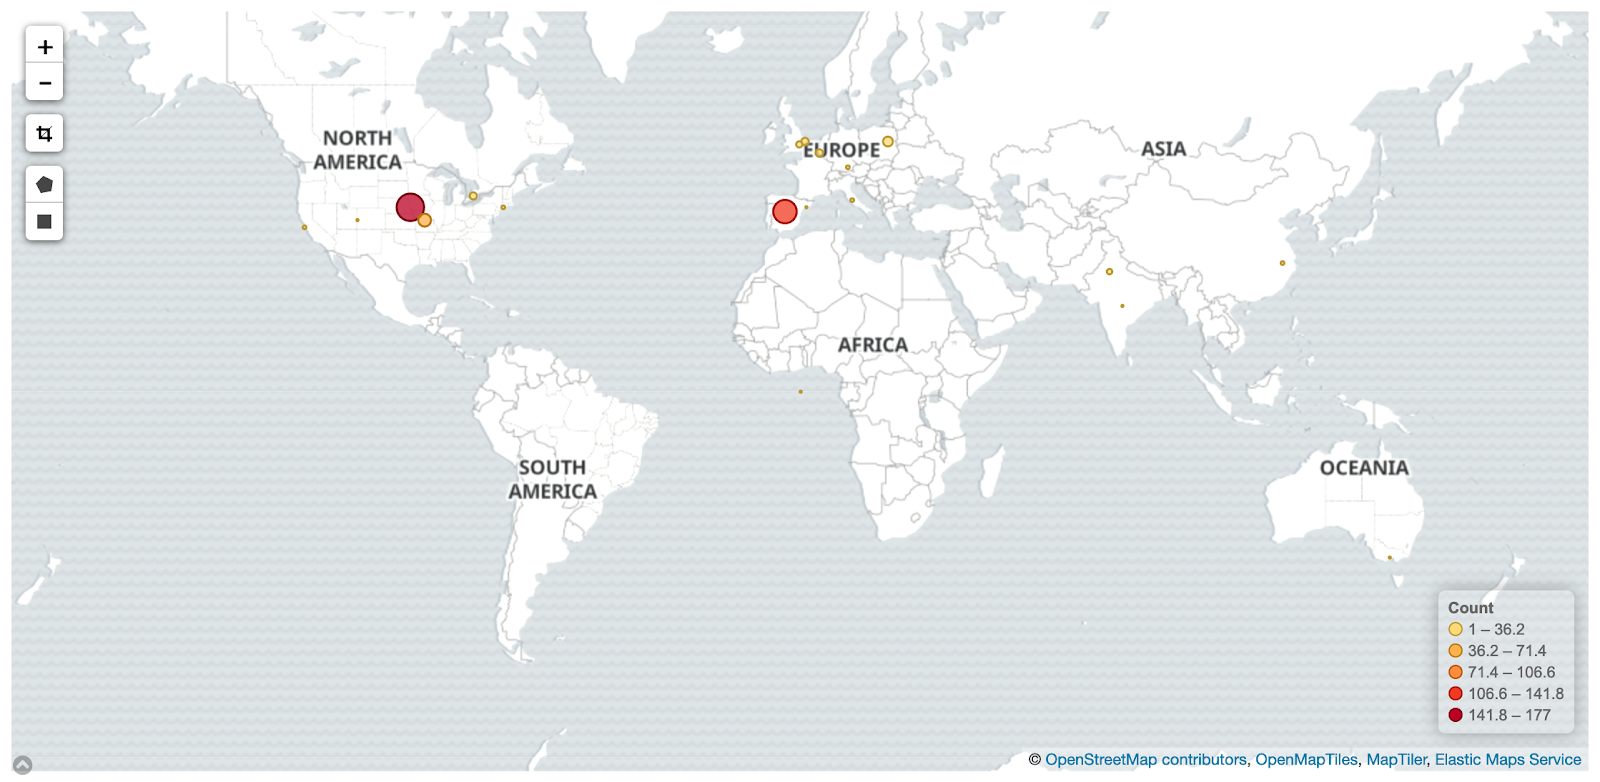
\includegraphics{images/contributor-location_dot-density-map.png}

Source:
\href{https://chaoss.biterg.io/goto/a62f3584a41c1c4c1af5d04b9809a860}{\url{https://chaoss.biterg.io/goto/a62f3584a41c1c4c1af5d04b9809a860}}

Visual heat map:

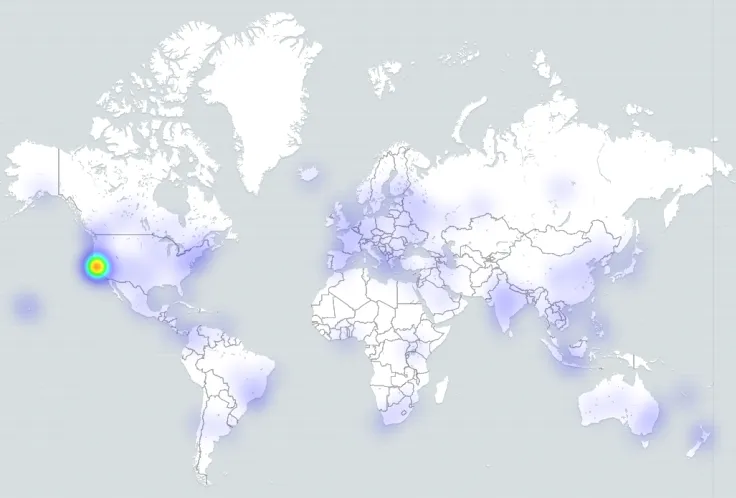
\includegraphics{images/contributor-location_heatmap.png}

Source:
\href{https://blog.bitergia.com/2018/11/20/ubers-community-software-development-analytics-for-open-source-offices}{\url{https://blog.bitergia.com/2018/11/20/ubers-community-software-development-analytics-for-open-source-offices}}

\hypertarget{tools-providing-the-metric}{%
\subsubsection{Tools providing the
metric}\label{tools-providing-the-metric}}

\begin{itemize}
\tightlist
\item
  GrimoireLab
\item
  Augur
\end{itemize}

\hypertarget{data-collection-strategies}{%
\subsubsection{Data Collection
Strategies}\label{data-collection-strategies}}

Different approaches can be used to collect information about location:

\begin{itemize}
\tightlist
\item
  Collect the location information from a contributor's profile in the
  system of engagement.
\item
  Use IP address geolocation of the most frequent locations that
  contributions are made.
\item
  Infer geographical location from the timestamp in contributions.
\item
  Survey contributors.
\end{itemize}

The key challenge for collecting data is determining the location of the
contributor. Best practice would be to leverage any profile information
available from the system of engagement, and if that is not available
then use IP geolocation to determine the most frequent location of
contribution from that individual. Note that contributors may enter in
their profile information false or nonsensical location information
(e.g., ``Earth'' or ``Internet''). Note that IP geolocation can provide
large numbers of false positives due to use of VPNs or other IP masking
tools.

An additional consideration would be the use of external data collection
tools such as community surveys or event registration data that could
cross reference systems of engagement profiles. Contributor location
data could be collected inline with event
\href{https://chaoss.community/metric-attendee-demographics/}{attendee
demographics} and
\href{https://chaoss.community/metric-speaker-demographics/}{speaker
demographics}.

\hypertarget{references}{%
\subsection{References}\label{references}}

\begin{itemize}
\tightlist
\item
  Gonzalez-Barahona, J. M., Robles, G., Andradas-Izquierdo, R., \&
  Ghosh, R. A. (2008). Geographic origin of libre software developers.
  \emph{Information Economics and Policy}, \emph{20}(4), 356-363.
\end{itemize}
 
\hypertarget{contributors}{%
\section{Contributors}\label{contributors}}

Question: Who are the contributors to a project?

\hypertarget{description}{%
\subsection{Description}\label{description}}

A contributor is defined as anyone who contributes to the project in any
way. This metric ensures that all types of contributions are fully
recognized in the project.

\hypertarget{objectives}{%
\subsection{Objectives}\label{objectives}}

Open source projects are comprised of a number of different
contributors. Recognizing all contributors to a project is important in
knowing who is helping with such activities as code development, event
planning, and marketing efforts.

\hypertarget{implementation}{%
\subsection{Implementation}\label{implementation}}

Collect author names from collaboration tools a project uses.

\textbf{Aggregators:}

\begin{itemize}
\tightlist
\item
  Count. Total number of contributors during a given time period.
\end{itemize}

\textbf{Parameters:}

\begin{itemize}
\tightlist
\item
  Period of time. Start and finish date of the period. Default: forever.
  Period during which contributions are counted.
\end{itemize}

\hypertarget{filters}{%
\subsubsection{Filters}\label{filters}}

By location of engagement. For example:

\begin{itemize}
\tightlist
\item
  Commit authors
\item
  Issue authors
\item
  Review participants, e.g., in pull requests
\item
  Mailing list authors
\item
  Event participants
\item
  IRC authors
\item
  Blog authors
\item
  By release cycle
\item
  Timeframe of activity in the project, e.g, find new contributors
\item
  Programming languages of the project
\item
  Role or function in project
\end{itemize}

\hypertarget{visualizations}{%
\subsubsection{Visualizations}\label{visualizations}}

\begin{itemize}
\tightlist
\item
  List of contributor names (often with information about their level of
  engagement)
\end{itemize}

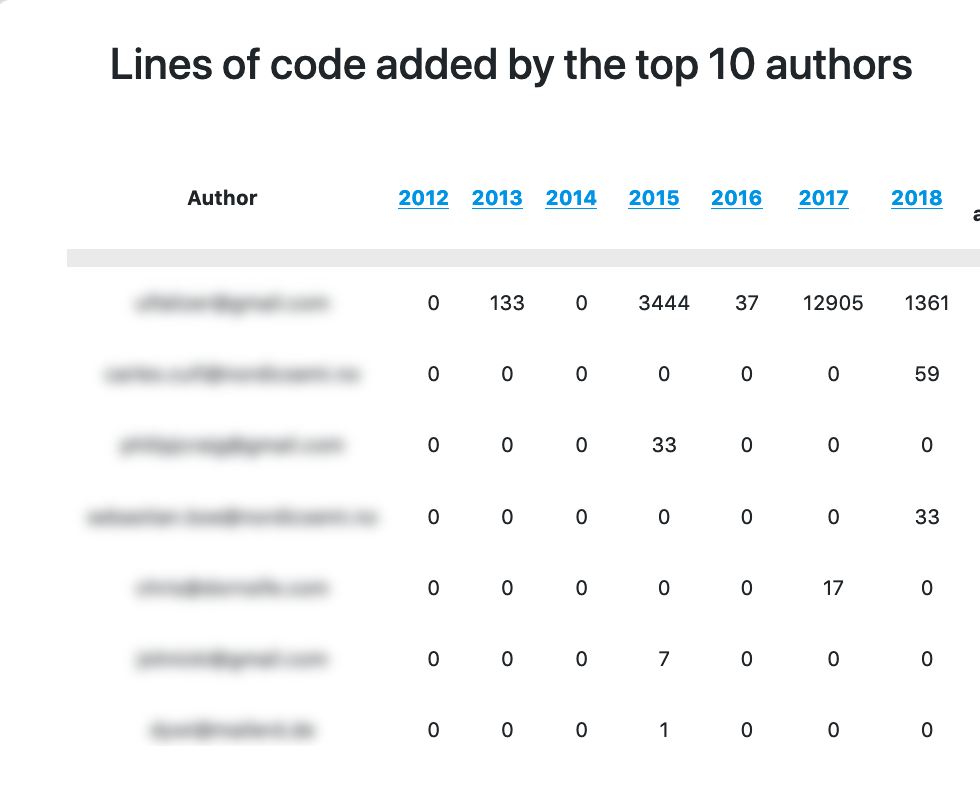
\includegraphics{images/contributors_top-contributor-info.png}

\begin{itemize}
\tightlist
\item
  Summary number of contributors
\end{itemize}

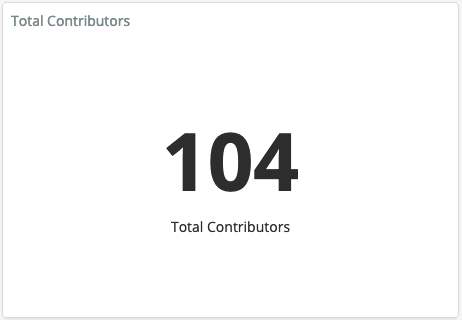
\includegraphics{images/contributors_summary-contributor-number.png}

\begin{itemize}
\tightlist
\item
  Change in the number of active contributors over time
\end{itemize}

\includegraphics{images/contributors_growth.png}

\begin{itemize}
\tightlist
\item
  New contributors (sort list of contributors by date of first
  contribution)
\end{itemize}

\includegraphics{images/contributors_first-commit-date.png}

\hypertarget{tools-providing-the-metric}{%
\subsubsection{Tools Providing the
Metric}\label{tools-providing-the-metric}}

\begin{itemize}
\tightlist
\item
  \href{https://chaoss.github.io/grimoirelab/}{GrimoireLab}
\item
  \href{http://augur.osshealth.io/api_docs/\#api-Evolution-Contributors_Repo_}{Augur}
\end{itemize}

\hypertarget{data-collection-strategies}{%
\subsubsection{Data Collection
Strategies}\label{data-collection-strategies}}

As indicated above, some contributor information is available via
software such as GrimoireLab and Augur. However, some contributor
insights are less easily obtained via trace data. In these cases,
surveys with community members or event registrations can provide the
desired information. Sample questions include:

\begin{itemize}
\tightlist
\item
  Interview question: Which contributors do not typically appear in
  lists of contributors?
\item
  Interview question: Which contributors are often overlooked as
  important contributors because their contributions are more ``behind
  the scenes''?
\item
  Interview question: What other community members do you regularly work
  with?
\end{itemize}

Additionally, surveys with community members can provide insight to
learn more about contributions to the project. Sample questions include:

\begin{itemize}
\tightlist
\item
  Likert scale {[}1-x{]} item: I am contributing to the project
\item
  Matrix survey item: How often do you engage in the following
  activities in the project?

  \begin{itemize}
  \tightlist
  \item
    Column headings: Never, Rarely(less than once a month), Sometimes
    (more than once a month), Often(once a week or more)
  \item
    Rows include: a) Contributing/reviewing code, b) Creating or
    maintaining documentation, c) Translating documentation, d)
    Participating in decision making about the project's development, e)
    Serving as a community organizer, f) Mentoring other contributors,
    g) Attending events in person, h) Participating through school or
    university computing programs, i) Participating through a program
    like Outreachy, Google Summer of Code, etc., j) Helping with the ASF
    operations (e.g., board meetings or fundraising)
  \end{itemize}
\end{itemize}

\hypertarget{references}{%
\subsection{References}\label{references}}
 
\hypertarget{organizational-diversity}{%
\section{Organizational Diversity}\label{organizational-diversity}}

Question: What is the organizational diversity of contributions?

\hypertarget{description}{%
\subsection{Description}\label{description}}

Organizational diversity expresses how many different organizations are
involved in a project and how involved different organizations are
compared to one another.

\hypertarget{objectives}{%
\subsection{Objectives}\label{objectives}}

\begin{itemize}
\tightlist
\item
  Get a list of organizations contributing to a project.
\item
  See the percentage of contributions from each organization within a
  defined period of time.
\item
  See the change of composition of organizations within a defined period
  of time.
\item
  Get a list of people that are associated with each organization.
\end{itemize}

\hypertarget{implementation}{%
\subsection{Implementation}\label{implementation}}

\begin{itemize}
\tightlist
\item
  Collect data from data sources where contributions occur.
\item
  Identify contributor affiliations to get a good estimate of which
  organizations they belong to.
\item
  Correlate information about contributions, assigning each to
  appropriate organization.
\item
  Depending on the needs of the project, you may want to consider such
  issues as how to handle multiple email addresses, affiliation changes
  over time, or contractor vs. employee.
\end{itemize}

\hypertarget{tools-providing-the-metric}{%
\subsubsection{Tools Providing the
Metric}\label{tools-providing-the-metric}}

\begin{itemize}
\tightlist
\item
  \href{https://chaoss.github.io/grimoirelab}{GrimoireLab} supports
  organizational diversity metrics out of the box. The
  \href{https://github.com/chaoss/grimoirelab-sortinghat}{GrimoireLab
  SortingHat} manages identities. The
  \href{https://github.com/chaoss/grimoirelab-hatstall}{GrimoireLab
  Hatstall} user interface allows correcting organizational affiliation
  of people and even recording affiliation changes.

  \begin{itemize}
  \tightlist
  \item
    View an example visualization on the
    \href{https://chaoss.biterg.io/app/kibana\#/dashboard/Community-Structure-by-Organization}{CHAOSS
    instance of Bitergia Analytics}.
  \item
    Download and import a ready-to-go dashboard containing examples for
    this metric visualization from the
    \href{https://chaoss.github.io/grimoirelab-sigils/panels/community-structure-by-organization/}{GrimoireLab
    Sigils panel collection}.
  \item
    Add a sample visualization to any GrimoreLab Kibiter dashboard
    following these instructions:

    \begin{itemize}
    \tightlist
    \item
      Create a new Pie chart

      \begin{itemize}
      \tightlist
      \item
        Select the \texttt{all\_onion} index
      \item
        Metrics Slice Size: \texttt{Sum} Aggregation,
        \texttt{contributions} Field, \texttt{Contributions} Custom
        Label
      \item
        Buckets Split Slices: \texttt{Terms} Aggregation,
        \texttt{author\_or\_name} Field, \texttt{metric:\ Contributions}
        Order By, \texttt{Descending} Order, \texttt{500} Size,
        \texttt{Organization} Custom Label
      \end{itemize}
    \item
      Example Screenshot
    \end{itemize}

    \includegraphics{images/organizational-diversity_piechart.png}
  \end{itemize}
\item
  \href{https://lfanalytics.io}{LF Analytics} provides organization
  diversity metrics in the primary view for commits, issues filed, and
  communication channels (current support for Slack and groups.io)
\end{itemize}

\includegraphics{images/organizational-diversity_lfanalytics-orgdiversity.png}

\hypertarget{data-collection-strategies}{%
\subsubsection{Data Collection
Strategies}\label{data-collection-strategies}}

\textbf{Qualitative}

\begin{itemize}
\tightlist
\item
  Footprint of an organization in a project or ecosystem
\item
  Influence of an organization in a project or ecosystem
\item
  Affiliation diversity in governance structures.
\end{itemize}

\textbf{Quantitative}

\begin{itemize}
\tightlist
\item
  \% of commits by each organization
\item
  \% of merges/reviews from each organization
\item
  \% of any kind of contributors from each organization
\item
  \% of lines of code contributed by each organization
\item
  \% issues filed by each organization
\item
  \href{https://github.com/chaoss/metrics/blob/master/activity-metrics/contributing-organizations.md}{Contributing
  Organizations} - What is the number of contributing organizations?
\item
  \href{https://github.com/chaoss/metrics/blob/master/activity-metrics/new-contributing-organizations.md}{New
  Contributing Organizations} - What is the number of new contributing
  organizations?
\item
  New Contributor Organizations - New organizations contributing to the
  project over time.
\item
  Number of Contributing Organizations - Number of organizations
  participating in the project over time.
\item
  Elephant Factor - If 50\% of community members are employed by the
  same company, it is the elephant in the room. Formally: The minimum
  number of companies whose employees perform 50\% of the commits
\item
  \href{https://github.com/chaoss/metrics/blob/master/activity-metrics/contributor-diversity.md}{Affiliation
  Diversity} - Ratio of contributors from a single company over all
  contributors. Also described as: Maintainers from different companies.
  Diversity of contributor affiliation.
\item
  In projects with the concept of code ownership, \% of code owners
  affiliated with each organization weighed by the importance/size/LoC
  of the code they own and the number of co-owners.
\end{itemize}

\hypertarget{references}{%
\subsection{References}\label{references}}

\begin{itemize}
\tightlist
\item
  Potential implementations and references:

  \begin{itemize}
  \tightlist
  \item
    \url{https://bitergia.gitlab.io/panel-collections/open_source_program_office/organizational-diversity.html}
  \item
    \href{https://katacontainers.biterg.io}{Kata Containers dashboard
    entry page} (bottom of this)
  \item
    \href{https://github.com/chaoss/augur}{Augur}
  \end{itemize}
\end{itemize}
 
 
 


\hypertarget{project-popularity}{%
\section{Project Popularity}\label{project-popularity}}

Question: How popular is an open source project?

\hypertarget{description}{%
\subsection{Description}\label{description}}

Project popularity can be measured by how much activity is visible
around a project. Popularity has a positive feedback loop in which more
popular projects get more attention, attract more users or developers,
and see increases in popularity, spinning the popularity wheel.

Project popularity may be used as a proxy for understanding project
value because open source project economic value is hard to measure, due
to a lack of available usage or sales information for open source
projects.

\hypertarget{objectives}{%
\subsection{Objectives}\label{objectives}}

In a quest to earn a living wage, and to maximize future employment
opportunities, workers may be interested in knowing which projects are
growing and are underserved. Similarly, from an organizational
perspective, knowing which projects are highly used can be helpful in
knowing which projects might be worth investing in. The Project
Popularity metric can be used to identify the trajectory of a project's
development.

\hypertarget{implementation}{%
\subsection{Implementation}\label{implementation}}

The project popularity metric is often considered with changes over
time. There are numerous example vectors to consider when measuring
project popularity based on the number of:

\begin{enumerate}
\def\labelenumi{\arabic{enumi}.}
\tightlist
\item
  Social media mentions
\item
  Forks
\item
  \href{https://chaoss.community/metric-change-requests/}{Change
  requests}
\item
  \href{https://chaoss.community/metric-issues-new/}{New Issues}
\item
  Stars, badges, likes
\item
  \href{https://chaoss.community/metric-new-contributors/}{New
  contributors}
\item
  \href{https://chaoss.community/metric-organizational-diversity/}{Organizational
  Diversity}
\item
  Job postings requesting skills in project
\item
  Conversations within and outside of project
\item
  Clones
\item
  Followers
\item
  Downstream dependencies
\item
  People attending events that focus on a project
\end{enumerate}

\hypertarget{visualizations}{%
\subsubsection{Visualizations}\label{visualizations}}

Issues and reviews (change requests) visualization from Cauldron
(GrimoireLab):

\includegraphics{images/project-popularity_issues-and-reviews.png}

Kubernetes project popularity statistics from DevStats:

\includegraphics{images/project-popularity_kubernetes.png}

\hypertarget{tools-providing-the-metric}{%
\subsubsection{Tools Providing the
Metric}\label{tools-providing-the-metric}}

\begin{itemize}
\tightlist
\item
  \href{https://github.com/chaoss/augur}{Augur}
\item
  \href{https://chaoss.github.io/grimoirelab/}{GrimoireLab}
\item
  \href{https://cauldron.io/}{Cauldron}
\end{itemize}

\hypertarget{references}{%
\subsection{References}\label{references}}

\begin{itemize}
\tightlist
\item
  \href{http://blog.honeypot.io/most-exciting-open-source-projects-2018/}{Popular
  OpenSource Projects}
\item
  \href{https://isitmaintained.com/}{Is It Maintained?}
\item
  \href{https://github.blog/2018-02-08-open-source-project-trends-for-2018/}{Open
  Source Project Trends}
\item
  \href{https://www.payscale.com/research/US/Skill=Kubernetes/Salary}{Kubernetes
  Salary}
\end{itemize}
 
\hypertarget{project-velocity}{%
\section{Project Velocity}\label{project-velocity}}

Question: What is the development speed for an organization?

\hypertarget{description}{%
\subsection{Description}\label{description}}

Project velocity is the number of issues, the number of pull requests,
volume of commits, and number of contributors as an indicator of
'innovation'.

\hypertarget{objectives}{%
\subsection{Objectives}\label{objectives}}

Gives an Open Source Program Office (OSPO) manager a way to compare the
project velocity across a portfolio of projects.

The OSPO manager can use the Project Velocity metric to:

\begin{itemize}
\tightlist
\item
  Report project velocity of open source projects vs in-house projects
\item
  Compare project velocity across a portfolio of projects
\item
  Identify which projects grow beyond internal contributors (when
  filtering internal vs. external contributors)
\item
  Identify promising areas in which to get involved
\item
  Highlight areas likely to be the successful platforms over the next
  several years
\end{itemize}

\href{https://www.cncf.io/blog/2017/06/05/30-highest-velocity-open-source-projects}{See
Example}

\hypertarget{implementation}{%
\subsection{Implementation}\label{implementation}}

Base metrics include:

\begin{itemize}
\tightlist
\item
  \href{https://github.com/chaoss/wg-evolution/blob/master/metrics/Issues_Closed.md}{issues
  closed}
\item
  \href{https://github.com/chaoss/wg-evolution/blob/master/metrics/Reviews.md}{number
  of reviews}
\item
  \href{https://github.com/chaoss/wg-evolution/blob/master/metrics/Code_Changes.md}{\#
  of code changes}
\item
  \href{https://github.com/chaoss/wg-risk/blob/master/metrics/Committers.md}{\#
  of committers}
\end{itemize}

\hypertarget{filters}{%
\subsubsection{Filters}\label{filters}}

\begin{itemize}
\tightlist
\item
  Internal vs external contributors
\item
  Project sources (e.g., internal repositories, open-source
  repositories, and competitor open-source repositories)
\item
  Time
\end{itemize}

\hypertarget{visualizations}{%
\subsubsection{Visualizations}\label{visualizations}}

\begin{itemize}
\tightlist
\item
  X-Axis: Logarithmic scale for Code Changes
\item
  Y-Axis: Logarithmic scale of Sum of Number of Issues and Number of
  Reviews
\item
  Dot-size: Committers
\item
  Dots are projects
\end{itemize}

\includegraphics{images/project-velocity_visualization.png}

\href{https://www.cncf.io/blog/2017/06/05/30-highest-velocity-open-source-projects/}{From
CNCF}

\hypertarget{tools-providing-the-metric}{%
\subsubsection{Tools providing the
Metric}\label{tools-providing-the-metric}}

\begin{itemize}
\tightlist
\item
  CNCF - \url{https://github.com/cncf/velocity}
\end{itemize}

\hypertarget{references}{%
\subsection{References}\label{references}}

\begin{itemize}
\tightlist
\item
  \href{https://www.threefivetwo.com/blog/can-open-source-innovation-work-in-the-enterprise}{Can
  Open Source Innovation work in the Enterprise?}
\item
  \href{https://www.nearform.com/blog/want-a-high-performing-culture-make-way-for-open-innovation}{Open
  Innovation for a High Performance Culture}
\item
  \href{https://www.cio.com/article/3213146/open-source-is-powering-the-digital-enterprise.html}{Open
  Source for the Digital Enterprise}
\item
  \href{https://www.cncf.io/blog/2017/06/05/30-highest-velocity-open-source-projects}{Highest
  Velocity Open Source Projects}
\end{itemize}
 
\hypertarget{social-listening}{%
\subsubsection{Social Listening}\label{social-listening}}

Question: How does one measure the value of community interactions and
accurately gauge ``reputation'' of a community as evident from
qualitative sentiment?

\emph{Note: This metric synthesizes several other metrics that can be
derived from trace data, and several process-oriented metrics. Embedded
footnotes annotate areas planned for later clarification, and questions
for later resolution.}

\hypertarget{description}{%
\paragraph{Description}\label{description}}

Social Listening is a combination of
\href{https://blog.hubspot.com/service/social-listening}{social
listening} practices across multiple channels along with a meaningful
set of categorizations. The combination of these tactics can lead to
systematic community analysis and can inform a community strategy that
leads to measurable business value. 1

\textbf{Theory and Origin}

Social currency or social capital is a social scientific theory. It
broadly considers how human interactions build relationships and trust
in a community. The Social Listening metric represents the reputation of
a community as measured via community trust, transparency, utility,
consistency, and merit.

Interpersonal relationships are the social fabric of communities. This
is shown in the
\href{https://theadminzone.com/ams/levingers-stage-theory.1272/}{Levinger's
Relationship Model} and
\href{https://psycnet.apa.org/record/1973-28661-000}{Social Penetration
Theory}. Community members' sense of personal and group identity grows
as they interact. Members build shared values, accumulate a sense of
trust, encourage cooperation, and garner reciprocity through acts of
\href{https://en.wikipedia.org/wiki/Self-disclosure}{self-disclosure}.
These interactions build an increased and measurable sense of
connection. The measure of these characteristics is called social
currency. 2

\textbf{Results}

The Social Listening metric is a way to sort through a fire hose of
qualitative data from community interactions. A central premise of this
approach is that community members' interactions have an impact on the
community. The Social Listening metric continually measures the
sentiment 3 from those interactions. It illustrates the reputation and
level of trust between community members and leaders. 4

\hypertarget{objectives}{%
\paragraph{Objectives}\label{objectives}}

Analyze the qualitative comments in community interactions. Gain an
overview of sentiment in a community. Get metrics that show at a glance
how a community is and was doing. Use lead metrics from continuous
measurements for proactive community strategy development. Instill trust
in community members that their thoughts and opinions are valued.

\hypertarget{implementation}{%
\paragraph{Implementation}\label{implementation}}

The Social Listening requires the collection of community comments
(communication traces), the definition of a codex, and the on-going
review of the communication traces. 5

Set up a Data Collection Platform of your choice as described in the
``Tools'' section below. Ensure it has a minimum of 4 dimensions and 3
communication channels. Once it is set up, the following method is used
to collect, analyze, and interpret results:

\includegraphics{images/social-listening_circle2.png}

\begin{enumerate}
\def\labelenumi{\arabic{enumi}.}
\item
  \textbf{Collect Communication Traces} -\/- Identify online platforms
  that your community is communicating on. Set up data funnels from the
  primary platform to your Social Listening tool. The critical data for
  the system is user generated content.
\item
  \textbf{Standardize How Communication Traces Should Be Assessed} -\/-
  Use a codex to define important concepts as a ``tracking keyword'' or
  ``category'' in the focal community. This unified codex of terms
  ensures consistent analysis as different people read and tag community
  sentiment. Formalizing the revision and addition structure to this
  codex on a regular basis is a must. 5
\item
  \textbf{Analyze the Communication Traces} -\/- Community sentiment is
  analyzed in the Social Listening tool by tagging data with codex
  terms. If the tagging is done by a team of people, it is recommended
  that everyone gets together regularly to discuss trends and ensure
  consistent tag use. If the tagging is done by an artificial
  intelligence algorithm, then a human team should supervise and retrain
  the AI as necessary. 5
\item
  \textbf{Share and Visualize the Aggregated Analysis} -\/- Visualize
  the quantitative count of codex terms over time, e.g., in a dashboard.
  This is where the qualitative analysis results produce an easy to
  observe dashboard of trends. Share analysis with team members. 6
\item
  \textbf{Benchmark, Set Goals \& Predict Future Growth} -\/- After
  getting enough data to form a benchmark, take stock of where your
  community stands. What are its strengths and weaknesses? What actions
  can be taken to make the community healthier and more robust? Then
  form community initiatives with well-defined goals and execute on
  these projects to affect the social currency metrics for next week. 6
\item
  \textbf{Repeat the Process} -\/- In regular evaluation meetings,
  discuss the shortcomings of the dataset or collection methods. Come up
  with methods to address these shortcomings in the future. Work
  solutions into the system and move forward. Truth is in the trend,
  power is in the pattern.7
\end{enumerate}

\hypertarget{filters}{%
\subparagraph{Filters}\label{filters}}

\begin{enumerate}
\def\labelenumi{\arabic{enumi}.}
\tightlist
\item
  \textbf{Channel}: Sort by where the data was collected from.
\item
  \textbf{Tag}: Show data based on what codex tags were used to identify
  sentiment in comments.
\item
  \textbf{Time}: Show trends in the data over time and pull specific
  data-sets.
\item
  \textbf{Most impactful comments}: Sort and filter by flags that can be
  placed in the data to highlight specific data points and explain their
  importance.
\item
  \textbf{AI vs. Human tagged}: Filter by whether tags were applied
  programmatically or by a person.
\item
  \textbf{Weighted currency:} Weight the ``importance'' of certain
  comments based on any one individually selected criteria. A resulting
  weighted view is simply a re-order of information based on weight.
\end{enumerate}

\hypertarget{visualizations}{%
\subparagraph{Visualizations}\label{visualizations}}

\textbf{Dashboard visualizing the aggregate metrics:}

\includegraphics{images/social-listening_dashboard.png}

\textbf{Example Social Listening tool:} On the left, raw community
comments are shown and tags are added in columns immediately to the
right. On the right, a pivot table shows in numbers how often tags
occurred in combination with other tags.

\includegraphics{images/social-listening_tool-example.png}

\textbf{Expanded comments view:} remove the ``quantitative'' from the
fields and provide the best possible way to read the different comments.

\includegraphics{images/social-listening_expanded-comment.png}

\hypertarget{tools-providing-the-metric}{%
\subparagraph{Tools Providing the
Metric}\label{tools-providing-the-metric}}

To implement the metric any MySQL, smart-sheet, excel, or airtable-like
excel datasheet program works fine. This data should be simplified
enough to interact with other data interfaces to ensure that data
migration is simple, straightforward, and can be automated (such as
google data studio). This requires that systems used to implement the
Social Listening metric work with CSV and other spreadsheet files, and
we heavily recommend open source programs for its implementation.

Once you have this, create a data set with the following data points: 8

\begin{longtable}[]{@{}ll@{}}
\toprule
Data Points & Description \\
\midrule
\endhead
Date of entry & Date data was imported to Social Listening tool \\
Date of comment & Date comment was made on original platform \\
Comment Text & Qualitative data brought in. Decide on how large you want
these chunks ported. Some may port an entire email while others will be
broken into one row per sentence. It should only have one
``sentiment'' \\
Data channel & Originating data channel the comment came from \\
Tags (created on codex document below) & Based on the unified codex of
terms, decide what tags to track. There can be two kinds of tags. On the
one hand, tags can be based on ``themes'' or recurring sentiment that
people voice (e.g., gamer gate, flamewar, or thank you notes). On the
other hand, tags based on ``categories'' can describe different aspects
of a community that members comment on (e.g., events, release, or
governance). \\
Social Currency Metric & The social currency being awarded or demerited
in the system. This will directly affect numbers. \\
Weighted Score & Once you've decided what your ``weight'' will be, you
can assign a system of -3 to +3 to provide a weighted view of
human-tagged metrics (AI will not assign a weight for several reasons).
This enables the ``most impactful comment'' filter. \\
\bottomrule
\end{longtable}

Create a second sheet for the Unified Codex of Terms which will define
terms. It should look like this: 8

\begin{longtable}[]{@{}llll@{}}
\toprule
Category Term & Definition & When to use & When not~to use \\
\midrule
\endhead
{[}Custom Tags - themes and categories{]} & & & \\
{[}Community specific jargon{]} & & & \\
Social Currency Dimensions: & & & \\
TRANSPARENCY & Do people recognize and feel a connection to your
community?~ & When they have the "words" to pinpoint why they feel you
are authentic or personable. & This is not about good customer service,
or doing well. That is utility. This is about whether they understand
who you are as a business and show they are onboard with it. \\
UTILITY & Is your community doing something useful or is it contributing
value? & Provide parameters that exclude when the term is used so that
people know when the category tag should not be implemented. & This is
not about good customer service, or doing well. That is utility. This is
about whether they understand who you are as a business and show they
are onboard with it. \\
CONSISTENCY & Do you have a history of being reliable and dependable? &
When they suggest they have used your brand, or interacted with you
several times & If they've only provided their comment to suggest you
were useful once, use utility instead. \\
MERIT & Does your community merit respect and attention for your
accomplishments? & When the social currency garnered from customers
seems it will continue for a while, and will impact other people's
opinions. & When they suggest they will use you again in the future use
trust instead as that is a personal trust in the brand. Merit is
external. \\
TRUST & Can people trust that your community will continue to provide
value and grow in the future? & When they suggest they trust you well
enough to continue conversations with you in the future & When there is
not substantial enough evidence to suggest they will continue to work
with and trust you as a loyal customer or community member. \\
INTERNAL REPUTATION 9 & Do people believe these things strongly enough
to warrant conversation or action? & & \\
EXTERNAL REPUTATION 9 & What amount of your reputation in your community
is transferable to strangers outside of your community (cold audiences)?
& & \\
\bottomrule
\end{longtable}

The codex is filled in by stakeholders on a regular basis by specific
communities and forms the basis for analysis of the data. This is the
MOST IMPORTANT part. Without this the subjectivity of qualitative data
does not follow the rule of generalization: 9

\begin{quote}
``A concept applies to B population ONLY SO FAR AS C limitation.''
\end{quote}

\hypertarget{data-collection-strategies}{%
\subparagraph{Data Collection
Strategies}\label{data-collection-strategies}}

Community member comments are available from trace data. The Social
Listening metric ideally imports the comment text automatically into a
tool for tagging. Trace data can be collected from a communities'
collaboration platforms where members write comments, including
ticketing systems, code reviews, email lists, instant messaging, social
media, and fora.

\textbf{Legal and Regulatory Considerations}

\emph{Points of destruction}: Detailed data is destroyed after \emph{xx}
months has passed. Quantitative calculations are kept for up to 250
weeks per GDPR compliance. Data older than 250 weeks becomes archived
data you cannot manipulate but can see. Users can negotiate the primary
statistic.

\hypertarget{references}{%
\paragraph{References}\label{references}}

\begin{itemize}
\tightlist
\item
  \href{https://airtable.com/invite/l?inviteId=inv8u49VVMtQTrfFU\&inviteToken=c49b1ed3759c5cd736901fd81c9f460f86e8e9f462703c4f85a3bdd7250ca5a7}{An
  example implementation on airtable}
\item
  \href{https://datastudio.google.com/open/1X9UdQz8FtHHmjMBpjba3pFqE55lNpwg5}{An
  example implementation in data studio}(report)
\item
  \href{https://datastudio.google.com/open/1Z4EJ03898lZxm2NZVULaEoLS0bYqL79A}{An
  example implementation in data studio} (data source)
\item
  \href{https://drive.google.com/open?id=1zi3JE0bwfEdRdc-wQEZn8GaB7sE8IvxeSeqvVywKnXw}{An
  example implementation in google sheets}
\item
  \href{https://docs.google.com/document/d/1RlAedRBQbhq0oYMCB3VqdawOCZE2XT5R3teydjBZODM/edit\#heading=h.8hyunaadfriq}{Implementation
  documentation} (starts on page 33)
\end{itemize}

\hypertarget{annotated-footnotes}{%
\paragraph{Annotated Footnotes}\label{annotated-footnotes}}

1 CHAOSS metrics historically is to create standard definitions that can
be used reliably across projects to support comparisons. This metric may
evolve into a project in the future.

2 What metrics emerge from this description? Likely included are: 1.
community trust, 2. transparency, 3. utility, 4. consistency, and 5.
merit

3 Analysis of sentiment suggests that metric (6) is likely
"Communications Sentiment", and the definition may need to include
references to common sentiment analysis tools, sometimes called "bags of
words".

4 Measuring how trust trust is instilled in community members, such that
their thoughts and opinions are valued is likely metric (7) that will
define a process, and perhaps is not measurable via trace data.

5 A substantial portion of any codex for open source software will be
common across projects, and each project is likely to have a set of
particular interests that are a subset of that codex. In some cases,
their main interests may not be present in an established codex
component. In general, the codex, like the CHAOSS project itself, is
open sourced as shared metadata to ensure shared understanding across
open source communities.

6 This describes the evolution of a standard codex, and its elements
through the process of CHAOSS working groups and projects, characterized
in the previous footnote. Likely this will be a process metric (8).

7 Candidate process oriented metric (9).

8 Examples of data coded using the open sourced codex, as it evolves,
will be essential components for advancing open source software through
Social Listening. Implementations will require these examples, and their
provision as open source assets of the CHAOSS project will return value
as shared data.

9 Internal and external reputation are likely metrics (10), and (11)
arising from the Social Listening metric.
 
 

\hypertarget{job-opportunities}{%
\section{Job Opportunities}\label{job-opportunities}}

Question: How many job postings request skills with technologies from a
project?

\hypertarget{description}{%
\subsection{Description}\label{description}}

A common way for open source contributors to earn a living wage is to be
employed by a company or be a self-employed or freelance developer.
Skills in a specific project may improve a job applicant's prospects of
getting a job. The most obvious indicator for demand related to a skill
learned in a specific open source project is when that project or its
technology is included in job postings.

\hypertarget{objectives}{%
\subsection{Objectives}\label{objectives}}

The metric gives contributors a sense of how much skills learned in a
specific open source project are valued by companies.

\hypertarget{implementation}{%
\subsection{Implementation}\label{implementation}}

To obtain this metric on a job search platform (e.g., LinkedIn, Indeed,
or Dice), go to the job search and type in the name of the open source
project. The number of returned job postings is the metric. Periodically
collecting the metric through an API of a job search platform and
storing the results allows to see trends.

\hypertarget{filters}{%
\subsubsection{Filters}\label{filters}}

\begin{itemize}
\tightlist
\item
  Age of job posting; postings get stale and may not be removed when
  filled
\end{itemize}

\hypertarget{visualizations}{%
\subsubsection{Visualizations}\label{visualizations}}

The metric can be extended by looking at:

\begin{itemize}
\tightlist
\item
  Salary ranges for jobs returned
\item
  Level of seniority for jobs returned
\item
  Availability of jobs like on-site or off-site
\item
  Location of job
\item
  Geography
\end{itemize}

\hypertarget{references}{%
\subsection{References}\label{references}}

\begin{itemize}
\tightlist
\item
  LinkedIn Job Search API:
  \url{https://developer.linkedin.com/docs/v1/jobs/job-search-api\#}
\item
  Indeed Job Search API:
  \url{https://opensource.indeedeng.io/api-documentation/docs/job-search/}
\item
  Dice.com Job Search API:
  \url{http://www.dice.com/external/content/documentation/api.html}
\item
  Monster Job Search API: \url{https://partner.monster.com/job-search}
\item
  Ziprecruiter API (Requires Partnership):
  \url{https://www.ziprecruiter.com/zipsearch}
\end{itemize}

\emph{Note:} This metric is limited to individual projects but
engagement in open source can be beneficial for other reasons. This
metric could be tweaked to look beyond a single project and instead use
related skills such as programming languages, processes, open source
experience, or frameworks as search parameters for jobs.
 
\hypertarget{organizational-project-skill-demand}{%
\subsubsection{Organizational Project Skill
Demand}\label{organizational-project-skill-demand}}

Question: How many organizations are using this project and could hire
me if I become proficient?

\hypertarget{description}{%
\paragraph{Description}\label{description}}

Organizations engage with open source projects through use and
dependencies. This metric is aimed at determining downstream demand of
skills related to an open source project. This metric looks at
organizations that deploy a project as part of an IT infrastructure,
other open source projects with declared dependencies, and references to
the project through social media, conference mentions, blog posts, and
similar activities.

\hypertarget{objectives}{%
\paragraph{Objectives}\label{objectives}}

As a developer, I'd like to invest my skills and time in a project that
has a likelihood of getting me a decent paying job in the future. People
can use the Downstream Organizational Impact of a Project Software
metric to discover which projects are used by organizations, and they
may, therefore, be able to pursue job opportunities with, possibly
requiring IT support services.

\hypertarget{implementation}{%
\paragraph{Implementation}\label{implementation}}

Base metrics include:

\begin{itemize}
\tightlist
\item
  Number of organizations that created issues for a project
\item
  Number of organizations that created pull requests for a project
\item
  Number of organizations that blog or tweet about a project
\item
  Number of organizations that mention a project in open hiring requests
\item
  Number of organizations that are represented at meetups about this
  project
\item
  Number of other projects that are dependent on a project
\item
  Number of books about a project
\item
  Google search trends for a project
\end{itemize}

\hypertarget{visualizations}{%
\subparagraph{Visualizations}\label{visualizations}}

The following visualization demonstrates the number of downstream
projects dependendent on the project in question. While this
visualization does not capture the entirety of the Downstream
Organizational Impact of a Project Software metric, it provides a visual
for a portion.

\includegraphics{images/organizational-project-skill-demand_paper.png}

Other visualizations could include Google search trends (React vs.
Angular vs. Vue.js)

\includegraphics{images/organizational-project-skill-demand_google-trends.png}

ThoughtWorks publishes a series called 'Tech Radar' that shows the
popularity of technologies.

\includegraphics{images/organizational-project-skill-demand_tech-radar.png}

Tech Radar allows you to drill down on projects to see how the
assessment has changed over time.

\includegraphics{images/organizational-project-skill-demand_tech-react.png}

StackOverview publishes an annual developer's survey

\includegraphics{images/organizational-project-skill-demand_stack-overflow.png}

\hypertarget{tools-providing-the-metric}{%
\subparagraph{Tools Providing the
Metric}\label{tools-providing-the-metric}}

\begin{itemize}
\tightlist
\item
  Google Trends - for showing search interest over time
\item
  ThoughtWorks TechRadar - project assessments from a tech consultancy
\item
  StackOverflow Developer's Survey - annual project rankings
\item
  Augur; Examples are available for multiple repositories:

  \begin{itemize}
  \tightlist
  \item
    \href{http://augur.osshealth.io/repo/Rails\%20(wg-value)/rails/overview}{Rails}
  \item
    \href{http://augur.osshealth.io/repo/Zephyr-RTOS/zephyr/overview}{Zephyr}
  \item
    \href{http://augur.osshealth.io/repo/Apache\%20(wg-value)/cloudstack/overview}{CloudStack}
  \end{itemize}
\end{itemize}

\hypertarget{references}{%
\paragraph{References}\label{references}}

\begin{itemize}
\tightlist
\item
  \href{https://opensource.org/sponsors}{Open Source Sponsors}
\item
  \href{https://opensource.com/article/19/1/fiscal-sponsors-open-source}{Fiscal
  Sponsors and Open Source}
\item
  \href{https://www.networkworld.com/article/2867020/big-names-like-google-dominate-open-source-funding.html}{Large
  Corporate OpenSource Sponsors}
\item
  \href{https://www.npmjs.com/package/google-trends-api}{Google Trends
  API}
\item
  \href{https://aisel.aisnet.org/cgi/viewcontent.cgi?article=1496\&context=amcis2018}{Measuring
  Open Source Software Impact}
\item
  \href{https://www.thoughtworks.com/radar}{ThoughtWorks Tech Radar}
\item
  \href{https://insights.stackoverflow.com/survey/2019\#technology}{Stack
  Overflow Developer's Survey}
\end{itemize}
 
 
 

\end{document}